%
%  untitled
%
%  Created by Julian Sackmann on 2012-07-24.
%  Copyright (c) 2012 __MyCompanyName__. All rights reserved.
%
\documentclass[]{article}

% Use utf-8 encoding for foreign characters
\usepackage[utf8]{inputenx}

% Setup for fullpage use
\usepackage{fullpage}

% Uncomment some of the following if you use the features
%
% Running Headers and footers
\usepackage{fancyhdr}
\usepackage{lastpage}

% Multipart figures
%\usepackage{subfigure}

% More symbols
\usepackage{amsmath}
\usepackage{amssymb}
%\usepackage{latexsym}

% Surround parts of graphics with box
\usepackage{boxedminipage}

% Package for including code in the document
\usepackage{listings}

% If you want to generate a toc for each chapter (use with book)
\usepackage{minitoc}

% This is now the recommended way for checking for PDFLaTeX:
\usepackage{ifpdf}

\usepackage{indentfirst}
\usepackage{footnote}
\usepackage{multicol}
\usepackage{mathtools}
\usepackage{algorithm2e}


\ifpdf
\usepackage[pdftex]{graphicx}
\else
\usepackage{graphicx}
\fi
\title{Teóricas de Ingeniería del Software}
\author{ Julián Sackmann }

\date{10 de Septiembre de 2012}

\pagestyle{fancy}
\thispagestyle{fancy}
\addtolength{\headheight}{12pt}
\addtolength{\headsep}{0.3cm}
\lhead{Ingeniería del Software I}
\rhead{Julián Sackmann}
\cfoot{P\'agina \thepage\ de \pageref{LastPage}}
\renewcommand{\footrulewidth}{0.4pt}
\setcounter{page}{0}


\begin{document}

\ifpdf
\DeclareGraphicsExtensions{.pdf, .jpg, .tif}
\else
\DeclareGraphicsExtensions{.eps, .jpg}
\fi

%\setcounter{secnumdepth}{5}
\setcounter{tocdepth}{4}

\newcommand{\ig}[2]{
\begin{center}
	\includegraphics[scale=#1]{#2}
\end{center}}
\newcommand{\subsubsubsection}[1]{\paragraph{#1}~\newline
 \indent }
\newcommand{\subsubsubsubsection}[1]{\subparagraph{#1}}
\newcommand{\flecha}[1]{\xrightarrow{\hspace*{0.3cm} #1 \hspace*{0.3cm}}}
\newcommand{\Flecha}[1]{\xRightarrow{\hspace*{0.3cm} #1 \hspace*{0.3cm}}}
\newcommand{\caja}[2]{\begin{center}
	\fbox{
		\parbox{#1\linewidth}{
			#2
		}
	}
\end{center}}
\renewcommand\contentsname{Índice}





\begin{titlepage}

\newcommand{\HRule}{\rule{\linewidth}{0.5mm}} % Defines a new command for the horizontal lines, change thickness here

\center % Center everything on the page

%----------------------------------------------------------------------------------------
%	HEADING SECTIONS
%----------------------------------------------------------------------------------------

\textsc{\LARGE Universidad de Buenos Aires}\\[1.5cm] % Name of your university/college
\textsc{\Large Facultad de Ciencias exactas y Naturales}\\[0.5cm] % Major heading such as course name
\textsc{\large Licenciatura en Ciencias de la computación}\\[0.5cm] % Minor heading such as course title

%----------------------------------------------------------------------------------------
%	TITLE SECTION
%----------------------------------------------------------------------------------------

\HRule \\[0.4cm]
{ \huge \bfseries Teóricas de Ingeniería del Software I}\\[0.4cm] % Title of your document
\HRule \\[1.5cm]

%----------------------------------------------------------------------------------------
%	AUTHOR SECTION
%----------------------------------------------------------------------------------------
%
% \begin{minipage}{0.4\textwidth}
% \begin{flushleft} \large
% \emph{Autor:}\\
% Julián \textsc{Sackmann} % Your name
% \end{flushleft}
% \end{minipage}
% ~
% \begin{minipage}{0.4\textwidth}
% \begin{flushright} \large
% \emph{} \\
%  \textsc{} % Supervisor's Name
% \end{flushright}
% \end{minipage}\\[4cm]

% If you don't want a supervisor, uncomment the two lines below and remove the section above
\Large \emph{Autor:}\\
Julián \textsc{Sackmann}\\[2cm] % Your name

%----------------------------------------------------------------------------------------
%	DATE SECTION
%----------------------------------------------------------------------------------------

{\large 10 de Septiembre de 2012}\\[2cm] % Date, change the \today to a set date if you want to be precise

%----------------------------------------------------------------------------------------
%	LOGO SECTION
%----------------------------------------------------------------------------------------

\begin{minipage}[t]{\textwidth}
    \begin{minipage}[t]{.55 \textwidth}
        
\includegraphics{logo_uba.jpg}
    \end{minipage}%%
    \begin{minipage}[b]{.45 \textwidth}
        \textbf{\textsf{Facultad de Ciencias Exactas y Naturales}} \\
        \textsf{Universidad de Buenos Aires} \\
        {\scriptsize %
        Ciudad Universitaria - (Pabell\'on I/Planta Baja) \\
            Intendente G\"uiraldes 2160 - C1428EGA \\
        Ciudad Aut\'onoma de Buenos Aires - Rep. Argentina \\
            Tel/Fax: (54 11) 4576-3359 \\
        http://exactas.uba.ar \\
        }
    \end{minipage}
\end{minipage}%

%
\includegraphics[scale=1]{logo_uba.jpg}\\[1cm] % Include a department/university logo - this will require the graphicx package
%
\includegraphics{logo_uba.jpg}\\[1cm] % Include a department/university logo - this will require the graphicx package

%----------------------------------------------------------------------------------------

\vfill % Fill the rest of the page with whitespace

\end{titlepage}



%\maketitle

\thispagestyle{fancy}

\tableofcontents

\newpage

\section{¿Qué es la Ingeniería del Software?}
Es una rama interdisciplinaria de la computación que se ocupa de construir un producto de software de \textbf{buena calidad}, considerando las restricciones pertinentes al caso (por ejemplo, presupuesto y tiempo disponible, escalabilidad, complejidad, etc). Notar que no sólo se acota al desarrollo del producto, sino de:

\begin{itemize}
	\item Crear una especificación (con distintos niveles de formalidad) del producto que se desea en base a las restricciones provistas.
	\item Desarrollarlo.
	\item Documentarlo.
	\item Testearlo.
	\item Mantenerlo.
\end{itemize}

Formalmente, de acuerdo a la IEEE: \textit{Software engineering is the application of a systematic, disciplined, quantifiable approach to the development, operation, and maintenance of software}.

\subsection{¿De qué se ocupa la Ingeniería del Software?}
\begin{itemize}
	\item Diseño, adaptación y medición de procesos.
	\item Gestión de proyectos (riesgos, factibilidad, toma de decisiones, planificación, etc).
	\item Diseño y operación de infraestructura para el proceso: ej. control de configuraciones.
	\item Análisis de requerimientos.
	\item Diseño (\textit{in-the-small} e \textit{in-the-large}).
	\item Selección y adquisición o desarrollo de componentes para re-uso e infraestructura de desarrollo.
	\item Verificación, Validación y Testing.
\end{itemize}

\newpage

\section{Modelos de Desarrollo}

Un modelo de desarrollo de software se define como \textbf{un marco de trabajo usado para estructurar, planear y controlar el proceso de desarrollo de un sistema de información}.

\subsection{Modelo en cascada}

En 1970, Royce propuso el \textbf{modelo en cascada} del desarrollo de software. Esencialmente, se concibe el proceso de desarrollo como una secuencia ordenada de pasos estrictamente controlados. En este modelo no se permiten revisiones o reformulaciones de cosas ya realizadas. Tradicionalmente los pasos involucrados en este modelo son:
\begin{itemize}
	\item Requerimientos.
	\item Diseño.
	\item Implementación.
	\item Integración.
	\item Validación.
	\item Instalación.
\end{itemize}

Este modelo tiene la ventaja de ser extremadamente simple y de tener un control muy férreo de las variables y restricciones involucradas. Por ejemplo, se puede decir que se asignan exactamente 2 semanas al Diseño y el modelo garantiza que no se vaya a ocupar más que eso (porque nunca se vuelve sobre lo mismo). Sin embargo, esa misma característica que provee la simpleza y elegancia del modelo es también la que causa su mayor deficiencia: la rigidez. Al mantener una estructura tan dura, no provee la versatilidad que en muchos casos es necesaria para un proceso de desarrollo.

\subsection{Modelo en espiral}

Para subsanar el problema de la rigidez del modelo en cascada, en el año 1988 Boehm propuso el \textbf{modelo en espiral}. Para lograr eso, este modelo concibe el desarrollo de software como una espiral infinita y creciente en donde cíclicamente se alternan períodos de:

\begin{center}
	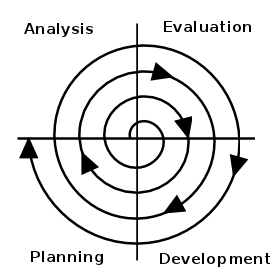
\includegraphics[scale=0.60]{Spiral.png}
\end{center}

En cada una de los períodos, se realizan las siguientes tareas:
\begin{itemize}
	\item Análisis: se determinan objetivos y se analizan restricciones.
	\item Evaluación: se evalúan distintas alternativas de diseño.
	\item Desarrollo: se desarrolla y testea la alternativa elegida en la iteración anterior.
	\item Planeamiento: se planea la iteración siguiente, considerando los problemas que hubo durante la evaluación y desarrollo de esta.
\end{itemize}

El problema que presenta este modelo es la dificultad en controlar las restricciones. Si bien en cada iteración se analizan las restricciones, no es trivial determinar cuántas iteraciones serán necesarias (o, mejor dicho, si se puede lograr el producto en una cantidad de iteraciones que no supere las restricciones).

%%NUEVO-COBY%%
El modelo de ingeniería en requerimientos planteado también por Boehm tiene el mismo ciclo de vida: una espiral infinita y creciente para la captura de requerimiento alternando elicitación, negociación, especificación y validación.
%%FIN-NUEVO-COBY%%

\subsection{Modelo en V}
El modelo en V, plantea	que el desarrollo de software sigue un modelo \textit{top-down} con dos series de fases, similares al modelo en cascada. La primer serie, llamada ``\textit{análisis, descomposición y diseño}'', comienza con un alto nivel de abstracción y en cada fase se va bajando el nivel de abstracción, trabajando sobre elementos sucesivamente más concretos.

Por el contrario, en la segunda serie, llamada ``\textit{testeo e integración}'' el nivel de abstracción va subiendo a medida que se avanza en las distintas fases.

Las fases por las que se atraviesa son:

\begin{center}
	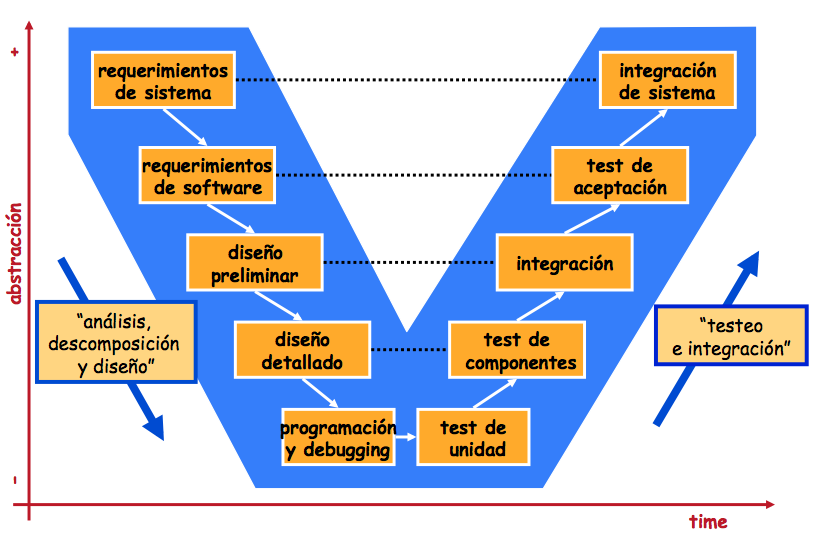
\includegraphics[scale=0.50]{Vmodel.png}
\end{center}

% \begin{minipage}[b]{0.5\linewidth}\centering
% 	\textbf{Análisis, descomposición y diseño}:
% 	\begin{itemize}
% 		\item Requerimientos de sistema.
% 		\item Requerimientos de software.
% 		\item Diseño preliminar.
% 		\item Diseño detallado.
% 		\item Programación y debugging.
% 	\end{itemize}
% \end{minipage}
% \begin{minipage}[b]{0\linewidth}\centering
% 	\textbf{Testeo e integración}:
% 	\begin{itemize}
% 		\item Test de unidad.
% 		\item Test de componentes.
% 		\item Integración.
% 		\item Test de aceptación.
% 		\item Integración de sistema.
% 	\end{itemize}
% \end{minipage}

Como se puede observar, el modelo recibe su nombre del hecho de que si se grafican las etapas en un gráfico de abstracción en función del tiempo, forman una V.

Este modelo presenta una relación simétrica entre los componentes que presentan igual grado de abstracción. En una determinada fase de la serie de \textit{testeo e integración} se realizan los tests correspondientes a la tarea que se haya diseñado en la fase de la serie \textit{análisis, descomposición y diseño} correspondiente al mismo nivel de abstracción.

Por ejemplo, en la fase de \textit{diseño preliminar}, se diseñan en abstracto, la interacción de las estructuras de datos a utilizarse dentro del programa, mientras que en \textit{diseño detallado}, el esfuerzo se concentra en el diseño específico de cada una de esas estructuras de datos. Durante la fase de \textit{test de componentes}, se testea la correctitud de cada estructura por separado, mientras que en la de \textit{integración} se testea la relación entre estructuras.

%%NUEVO-COBY%%
El ciclo de vida del testing dinámico tiene el mismo ciclo de vida en ``V'' y la misma relación de simtería entre cada etapa y su test (requerimientos con testing de sistema, diseño preliminar con testing de integración y diseño detallado con testing de unidad), con la diferencia de que al final de todo debe correrse el test de aceptación.
%%FIN-NUEVO-COBY%%

\subsection{Unified Software Development Process}
Propuesto por Jacobson en 1999.
\ig{0.5}{Jacobson.png}


\subsection{Twin Peaks}
El modelo \textit{Twin Peaks}, propone un modelo de exploración alternada entre la definición del problema y la definición de la solución, incrementando en cada salto, el nivel de detalle de cada una de las definiciones.

\begin{center}
	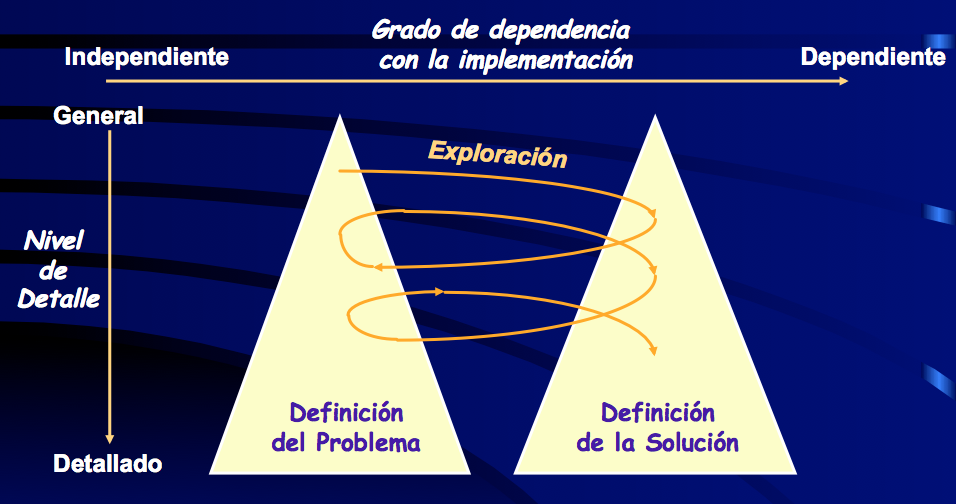
\includegraphics[scale=0.40]{TwinPeaks.png}
\end{center}

\newpage

\section{Modelo de Software}

En la Ingeniería del Software cobran un rol fundamental los \textbf{modelos de software}. Estos modelos son asiduamente utilizados porque permiten analizar un aspecto particular (o no) del problema. A su vez, permiten comunicar en forma precisa y ordenada aspectos relevantes tanto del problema como de la solución propuesta a otras personas.

Al trabajar con modelos se abaratan costos (construir una solución completa es en general notablemente más caro que un modelo) y se pueden detectar errores tempranamente en el proceso de desarrollo de una solución o producto.

Los modelos tienen 3 funciones claras:
\begin{itemize}
	\item \textbf{Abstrae}: permite al modelo enfocarse en un aspecto particular del problema, dejando de lado detalles irrelevantes al análisis (o de posterior solución).
	\item \textbf{Estructura}: simplifica y ordena el análisis.
	\item \textbf{Denota}: permite establecer la relación entre el mundo del documento y el mundo real.
\end{itemize}

Para la construcción de un buen modelo es necesario conocer el \textbf{propósito} del análisis.

En la ingeniería del software, a diferencia de otras disciplinas, el producto final (una pieza de software) es \textbf{intangible}. Esto implica que los modelos de software que se generan también son intangibles. Por esto, los modelos de software son \textbf{lenguajes formales} con una \textbf{denotación} precisa.

\subsection{Scope y Span}

Se define el \textbf{Scope} de un modelo como el tipo de fenómeno que se capta. Se relaciona con buscar seleccionar qué información se desea modelar y cuál ignorar. Básicamente, define el aspecto y alcance del modelo.

El \textbf{Span} de un modelo define el conjunto de individuos a los que describe. Influye fuertemente sobre cuánto debe alcanzar el modelo.

\subsection{Lenguaje Formal}

Un \textbf{Lenguaje Formal} se define como un lenguaje (sistema de comunicación estructurado) con símbolos y reglas para su combinación formalmente especificados. Tiene dos aspectos fundamentales
\begin{itemize}
	\item \textbf{Sintaxis}: define el conjunto de símbolos de representación utilizados.
	\item \textbf{Semántica}: define el subconjunto de reglas con las que se evitan accidentes sintácticos (por ejemplo, ambigüedades). En general existe una relación muy cercana entre la \textit{semántica} y la \textit{denotación} del modelo. Para definir la semántica, se pueden utilizar técnicas como:
	\begin{itemize}
		\item Definir una serie de reglas de traducción a otro lenguaje formal cuya sintáctica ya esté establecido.
		\item Definir un conjunto de relaciones (de equivalencia u orden) entre los distintos elementos sintácticos del lenguaje.
	\end{itemize}
\end{itemize}

La semántica de un lenguaje define una función que, dado un elemento de la sintaxis, devuelve un elemento (o subconjunto) del \textbf{dominio semántico} (conjunto de lexemas que pertenecen a un mismo campo de significación). Por ejemplo, en español, el dominio semántico de la palabra \textit{asiento} puede ser: \textit{silla}, \textit{sillón}, \textit{sofá}, etc.

Las reglas de transformación sintáctica deben mantener coherencia tanto con función de asignación al dominio semántico, como con la denotación y su correlación modelo-realidad. Una regla de transformación sintáctica es correcta si lleva dos elementos iguales en el modelo al mismo dominio semántico y a lo mismo en el mundo real.

Debido a que los problemas que se plantean en la computación suelen tener diversos aspectos con distintos objetivos y niveles de complejidad, y que cada modelo se enfoca en sólo un aspecto, suele ser necesario plantear no uno sino diversos modelos a la hora de modelar un sistema. Esto plantea el problema de la relación entre distintos modelos. Al ser modelos basados en lenguajes formales, idealmente, establecer una relación también debería tener un elevado grado de formalismo. Sin embargo, en la práctica es imposible vincular distintos modelos manteniéndolos analizables y entendibles. Es por esto que generalmente la relación entre modelos se da en lenguaje natural.

\newpage

\section{Validación, Verificación y Calidad}
La \textbf{validación} es un proceso cuyo objetivo es aumentar la confianza en que la \textit{denotación} del modelo es correcta. O sea que su descripción formal se corresponda con la realidad. Dado que involucra la realidad, necesariamente tiene que lidiar con informalidad. Más aún, debe establecer una noción de \textit{correctitud} entre un modelo formal y algo informal.

La \textbf{verificación} es un proceso cuyo objetivo es garantizar que una descripción formal es \textit{correcta} con respecto a otra. A diferencia de la validación, sólo involucra modelos formales. Sin embargo, la vinculación de los modelos no es trivial de formalizar. Si bien una vez formalizado se podrían generar pruebas automáticas, la complejidad (tanto espacial como temporal) de estas puede ser excesiva.

La \textbf{calidad} se define como el grado en el cual un software cumple con su propósito.

\newpage

\section{Ingeniería de Requerimientos}
Toda pieza de software se desarrolla con un \textbf{propósito} dentro de un \textbf{sistema}. El software es, en mayor o menor medida, un componente más del sistema. La \textbf{ingeniería de requerimientos} se ocupa, parcialmente, de la identificación y comprensión de dicho propósito. La ingeniería de requerimientos suele ser eficiente en sistemas \textit{intensivos} en software, es decir, sistemas en los que el componente de software del sistema cobra mucha relevancia.

Formalmente, se define a la ingeniería de requerimientos como: \textit{Un conjunto de actividades cuyo objetivo es identificar y comunicar el propósito de un sistema intensivo en software y los contextos en los que se utiliza. De esta forma, la ingeniería de requerimientos actúa como un puente entre las necesidades de los usuarios, clientes y otros entes involucrados en el uso del sistema y las capacidades y funciones que son factibles dadas las restricciones}.

Uno de los usos de la ingeniería de requerimientos es el de encontrar errores tempranamente en el desarrollo del software. Esto es extremadamente importante porque la detección de errores en forma temprana redunda en costos muy inferiores para su arreglo. Un error detectado, por ejemplo, durante el período de mantenimiento puede tener un costo 200 veces más elevado para su reparación que detectado en la etapa de requerimientos.

%%NUEVO-COBY%%
Otro de los usos de la ingeniería de requerimiento es la estructuración en modelos para facilitar la validación del producto a desarrollar (por ejemplo: la estructuración de objetivos para validar el propósito del producto en el modelo de objetivos, la estructuración en operaciones para validar que cada operación incluya requerimientos que inducirán a propósitos en el modelo de operaciones, etc).
%%FIN-NUEVO-COBY%%

\begin{center}
	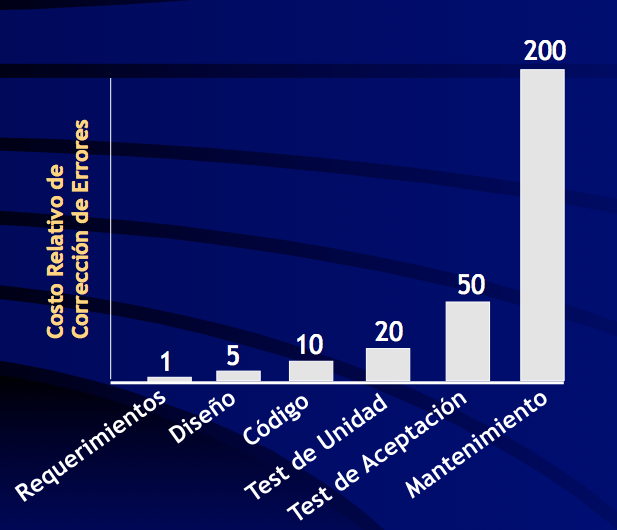
\includegraphics[scale=0.50]{Detec.png}
\end{center}

\subsection{Acerca de la Ingeniería de Requerimientos}
\subsubsection{Actividades de la Ingeniería de Requerimientos}
\begin{itemize}
	\item \textbf{Elicitación}: es el proceso de investigación durante el cual se entrevista a clientes, usuarios y otros \textit{stakeholders} con el objeto de obtener información sobre el sistema que quieren. A su vez se investiga el sistema y documentación existente (si hubiera). No es un proceso trivial dado que no siempre los \textit{stakeholders} tienen claro lo que quieren y muchas veces, aún cuando lo tienen claro no saben expresarlo.
	\item \textbf{Modelado}: es el proceso de documentación, de forma lo más rigurosa posible, de la información obtenida en la fase de elicitación. Tiene como objetivo abstraer los conceptos importantes y estructurarlos de forma conveniente.
	\item \textbf{Análisis}: es el proceso cuyo objetivo es verificar el modelo creado en la fase anterior. Se verifica tanto la coherencia interna como la coherencia entre modelos del mismo sistema.
	\item \textbf{Validación}: es el proceso en el cual se valida el modelo de la segunda fase (y el análisis de la tercera) contra el entendimiento que tenemos de la realidad.
	\item \textbf{Priorización}: es la fase en la que se comparan las distintas estrategias de alcance de objetivos, criterios de evaluación, criterios de los \textit{stakeholders}, etc.
	\item \textbf{Negociación}: es la fase en la que se discute con los \textit{stakeholders} sobre qué decisión es la apropiada, por qué motivos y cómo se unifican los criterios e intereses de cada una de las partes.
	\item \textbf{Especificación}: es el proceso de formalización del modelado. Hay que crear una documentación completa y detallada. Depende lo que se necesite, esta documentación puede ser para lectura, para un contrato, etc.
\end{itemize}

\subsubsection{Ciclo de vida}
Según Boehm la ingeniería de requerimientos presenta un ciclo de vida creciente en espiral similar al modelo de desarrollo:

\begin{center}
	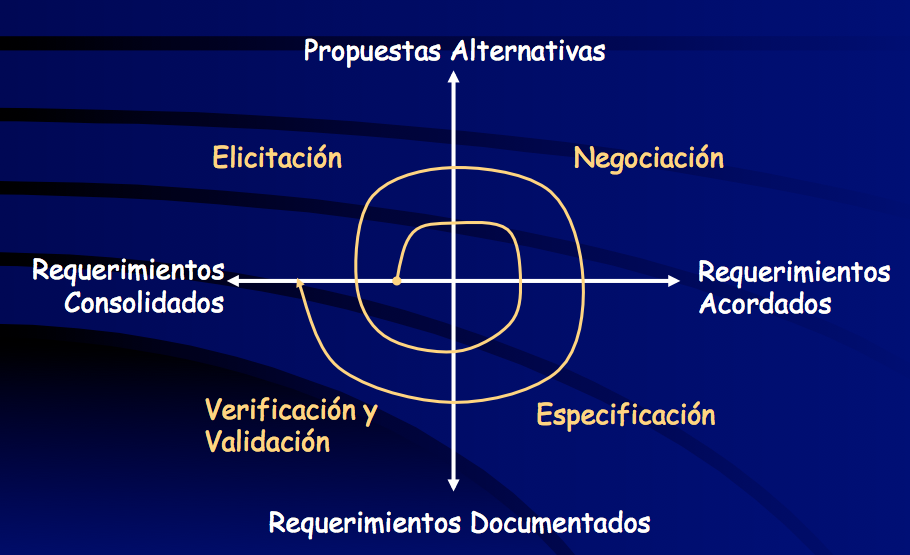
\includegraphics[scale=0.50]{IR_ciclo.png}
\end{center}

\subsubsection{Fenómenos, el mundo y la máquina}
La ingeniería de requerimientos trata los \textbf{fenómenos} que ocurren en el \textbf{mundo} y no en la \textbf{máquina}.
\begin{itemize}
	\item \textbf{Fenómeno}: es un hecho, situación o evento cuya existencia puede observarse.
	\item \textbf{Máquina}: es una porción del sistema a desarrollar o modificar.
	\item \textbf{Mundo}: es una porción del mundo, afectado por la máquina.
	\item \textbf{Interfaz}: es el punto de contacto entre la máquina y el mundo.
\end{itemize}

\subsubsection{Aserciones}
Una aserción se define como \textit{una afirmación, aseveración, expresión en que se da por cierta}. En la ingeniería de software se las categoriza en:
\begin{itemize}
	\item Aserciones \textbf{descriptivas}: definen cosas que son o presumimos ciertas en el mundo sobre el que trabajamos. En general son del tipo de restricciones de dominio.

%%NUEVO-COBY%%
Taxonomía de aserciones descriptivas: si son propiedades físicas son \emph{Propiedades del Dominio}; si son características aunque sujetas a cambios (por ejemplo: ``la moneda argentina es el peso'') se denominan \emph{Hipótesis del Dominio}.
%%FIN-NUEVO-COBY%%

	\item Aserciones \textbf{prescriptivas}: definen cosas que esperamos que vayan a ser ciertas una vez que sea afectado por nuestro sistema. Pueden ser de dos tipos:
	\begin{itemize}
		\item \textbf{Objetivos}: cosas que esperamos que vayan a ser ciertas \textbf{en el mundo} una vez que sea afectado por nuestro sistema (objetivos multiagente).
		\item \textbf{Requerimientos}: cosas que debemos hacer que sean ciertas\textbf{en la interfaz} (objetivos uniagentes).

%%NUEVO-COBY%%
Taxonomía de requerimientos: \emph{expectativa} (si el requerimiento es una asignación de responsabilidades a un agente externo) o \emph{requerimientos} (nuestro sistema deberá encargarse de cumplirlos).
%%FIN-NUEVO-COBY%%
	\end{itemize}

%%NUEVO-COBY%%
Para entender bien la diferencia entre Objetivo y Requerimiento: mientras que los objetivos son fenómenos globales (por ejemplo: ``prender el auto''), los requerimientos son objetivos uniagentes concretos (ejemplo: ``la bujía prende con una chispa el motor''). Un objetivo podría considerarse como muchos requerimientos haciendo algo para un fin mayor (el objetivo.)
%%FIN-NUEVO-COBY%%
\end{itemize}

\subsection{Modelo de Jackson}
El modelo de Jackson es una forma de operar con ingeniería de Requerimientos propuesta por Michael Jackson. Tiene una estructura que permite formular criterios de verificación:
\begin{itemize}
	\item Dadas las suposiciones de dominio (\textbf{D}), ¿los requerimientos (\textbf{R}) satisfacen los objetivos (\textbf{G})? \textbf{(R,D$\Rightarrow$G)}
	\item ¿El programa (\textbf{P}) corriendo sobre el hardware (\textbf{C}) satisface los requerimientos (\textbf{R})? \textbf{(P,C$\Rightarrow$R)}
\end{itemize}

Y numerosos de validación:
\begin{itemize}
	\item ¿Tenemos todos los objetivos? ¿Son objetivos válidos?
	\item ¿Todas las presunciones de dominio son verdaderas? ¿Existen presunciones de dominio relevantes que no hayamos considerado?
\end{itemize}

Se definen:
\begin{itemize}
	\item \textbf{Completitud} de un conjunto de requerimientos: están todos los requerimientos necesarios para lograr los objetivos.
	\item \textbf{Pertinencia} de un conjunto de requerimientos: no existe requerimientos que no ayuden a lograr los objetivos.
\end{itemize}

Este modelo garantiza la \textbf{completitud} de los requerimientos si:
\begin{itemize}
	\item Dado \textbf{D}, \textbf{R} garantiza \textbf{G}.
	\item \textbf{G} captura adecuadamente las necesidades de los stakeholders.
	\item \textbf{D} representa presunciones válidas acerca del mundo.
\end{itemize}

Es digno observar que evaluar el conjunto de presunciones del dominio no es un detalle menor. Si uno supone presunciones demasiado fuertes, si bien la construcción del sistema se economiza mucho, es demasiado propenso a fallas en el caso de que esas suposiciones no sean verdaderas. Por el contrario, presunciones demasiado débiles redundarán en un software robusto, pero potencialmente demasiado encarecido.


Jackson plantea no validar los requerimientos considerados contra el cliente, sino sólo los objetivos. Los requerimientos se deducen intrínsecamente de los objetivos. Para esta validación de objetivos el modelo extiende la definición de \textbf{completitud} y \textbf{pertinencia} a objetivos e intenta validar eso contra los stakeholders.


\subsection{Modelo de las 4 variables}
El modelo de las 4 variables fue propuesto por Parnas y Madey en 1995. Su característica predominante es que elabora la relación entre objetivos y requerimientos. Originalmente estaba orientado sólo a software de control.

Se introducen los conceptos de \textbf{Variables monitoreadas} (variables que el sistema sólo puede medir), \textbf{Variables controladas} (variables sobre las que el sistema tiene influencia), \textbf{Datos de salida} y \textbf{Datos de entrada}. A su vez, se dota al sistema de \textbf{sensores} (dispositivos encargados de sensar el entorno) y \textbf{actuadores} (dispositivos encargados de modificar el entorno).

Los requerimientos definen relaciones entre los datos de entrada y salida. Los objetivos relacionan variables monitoreadas y controladas, y se logran en la medida que los sensores y actuadores ``traducen'' correctamente datos y variables.

\subsection{Modelo de agentes}
%%NUEVO-COBY%%
Vimos el ``Diagrama de Contexto''.
%%FIN-NUEVO-COBY%%

El modelo de agentes intenta estructurar el mundo para poder manejar su enorme complejidad. Se define un \textbf{agente} como una entidad activa cumpliendo un rol determinado con capacidad de controlar o monitorear algún fenómeno del mundo (determinado por la interfaz). Puede ser un humano, un software, una máquina, etc, aunque no necesariamente hay una correlación 1 a 1: puede ser que un usuario determinado cumpla el rol de varios agentes (por ejemplo un humano que accede como usuario o como administrador).

Este modelo permite una representación gráfica conocida como \textit{diagramas de contexto}. En estos, se grafican a los distintos agentes involucrados en el sistema a modelar y los distintos fenómenos en la siguiente forma:

\begin{center}
	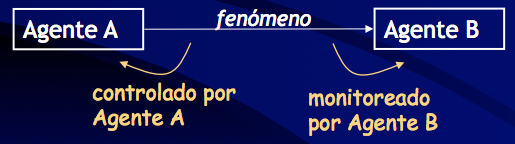
\includegraphics[scale = 0.70]{Contexto.png}
\end{center}

\subsection{Modelo de objetivos}
%%NUEVO-COBY%%
Vimos el ``Árbol de Objetivos''.
%%FIN-NUEVO-COBY%%


En el modelo de objetivos se define un \textbf{objetivo} como una aserción prescriptiva que el sistema deberá satisfacer a través de la cooperación de sus agentes. Esta aserción deberá estar dada en función de fenómenos en la \textbf{interfaz de agentes} (no necesariamente de la máquina). Los agentes deberán ajustar su comportamiento local de manera adecuada para garantizar el comportamiento global. Sólo podrán hacerlo dando garantías sobre la ocurrencia de fenómenos controlados por ellos mismos. La aserción deberá ser \textbf{declarativa} y no operacional. Es decir describir el objetivo a lograr y no cómo lograrlo.

\subsubsection{Diagrama de objetivos}
La forma de representar este modelo es mediante un \textbf{diagrama de objetivos}. Estos diagramas son un \textit{DAG}, donde casi todos los nodos son distintos tipos de aserciones. Un nodo puede ser un objetivo, una propiedad de dominio o un agente. Los ejes entre objetivos denotan contribuciones para satisfacción. Los ejes entre objetivos y agentes denotan asignación de responsabilidad.

%HABLAR DE REFINAMIENTOS
Los objetivos se grafican con un paralelogramo cuyo contenido (supongamos $Q$) denota el objetivo. Debe leerse ``\textit{Lograr el objetivo Q}''. La relación entre dos objetivos debe entenderse como ``\textit{El objetivo Q \textbf{contribuye} a lograr el objetivo P}''.

Los objetivos pueden ser categorizados en \textit{alto} o \textit{bajo} nivel en función de su grado de abstracción. Un objetivo de \textit{alto} nivel es más estratégico, de negocios. Por el contrario, los objetivos de \textit{bajo} nivel suelen ser más técnicos, ser más cercanos a las decisiones de diseño e involucrar menos agentes para su realización. En el caso extremo, en el que un objetivo tenga asociado un sólo agente \textbf{externo} se lo llama objetivo \textbf{uni-agente} o \textbf{expectativa}. Un \textbf{requerimiento} es un objetivo uni-agente que tiene que cumplir el sistema.

Se dice que un objetivo es \textbf{realizable} por un agente si:
\begin{itemize}
	\item El agente puede \textbf{monitorear} los fenómenos necesarios para satisfacer el objetivo.
	\item El agente puede \textbf{controlar} los fenómenos cuya ocurrencia necesita ser restringida para satisfacer el objetivo.
	\item No es necesario que el agente pueda conocer el futuro para garantizar el objetivo en el presente.
\end{itemize}

\subsubsubsection{Y-Refinamientos}
Para lograr un objetivo dado, a menudo es necesario haber realizado más de un objetivo previo; o sea, suele ser necesario que un objetivo sea \textit{refinado} por dos o más objetivos. Por eso, en el diagrama de objetivos se introduce la noción de \textbf{y-refinamiento}: una relación entre un objetivo y un conjunto de objetivos, en la cual todos los objetivos del conjunto \textit{contribuyen} a lograr el otro objetivo. Un y-refinamiento de $G$ en los nodos $G_1,G_2,...,G_n$ debe ser:
\begin{itemize}
	\item \textbf{Completo}: si la conjunción de todos los nodos $G_1,...,G_n$ y las presunciones de dominio $P$ lo implican. O sea, $G_1 \wedge G_2 \wedge ... \wedge G_n \wedge P \Rightarrow G$. Informalmente, si están satisfechos todos los objetivos $G_1,...,G_n$ y las presunciones de dominio son válidas, entonces $G$ es válido.
	\item \textbf{Mínimo (o minimal)}: si elimino cualquier objetivos $G_i$ de $G_1,...,G_n$, entonces dejo de poder inferir $G$.
	\item \textbf{Consistente}: si la conjunción de todos los objetivos $G_1,...,G_n$ y las presunciones de dominio $P$ no se contradicen. O sea $G_1 \wedge G_2 \wedge ... \wedge G_n \wedge P \not\Rightarrow False$.
\end{itemize}

\subsubsubsection{O-Refinamiento}
Los \textbf{o-refinamientos} permiten vincular un objetivo con un conjunto de y-refinamientos, proveyendo ``caminos'' alternativos para contribuir a lograr un objetivo dado.

También relacionado con la provisión de alternativas, existe la \textbf{O-Asignación de Responsabilidades}, que modela la asignación de responsabilidades alternativas a hojas del grafo a agentes.

\subsubsubsection{Refinamiento por hitos}
Los \textbf{refinamientos por hitos} (también llamado ``refinamiento por milestones'') son un caso particular de y-refinamiento, en el cual para lograr objetivo de la forma: \textit{Condición actual $\Rightarrow$ Condición esperada} se lo refina en dos objetivos de más bajo nivel:

\begin{center}
	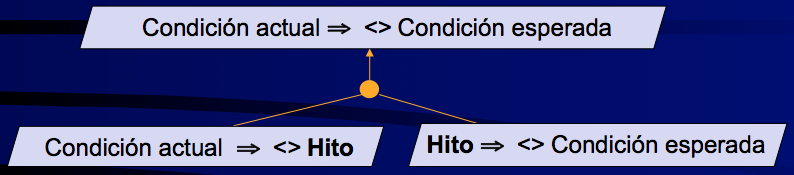
\includegraphics[scale=0.5]{Hitos.png}
\end{center}

De esta forma, se especifica, el ``paso intermedio'' por el que debe pasarse para pasar de la \textit{condición actual} a la \textit{esperada}. Observar que esta técnica es aplicable indistintamente del tipo de objetivo (\textit{lograr}, \textit{mantener}, \textit{evitar}, etc). Además, puede ser generalizada empleando $n$ hitos intermedios.

\subsubsubsection{Refinamiento por casos}
La técnica de \textbf{refinamiento por casos} es otro caso particular de y-refinamiento, que permite introducir \underline{objetivos complementarios}. Nuevamente, se aplica en objetivos de la forma \textit{Condición actual $\Rightarrow$ Condición esperada} (tanto \textit{lograr} como \textit{mantener}) y en los cuales haya una partición completa (aunque no necesariamente disjunta) en casos. Entonces, se refina el objetivo en dos objetivos de más bajo nivel:

\begin{center}
	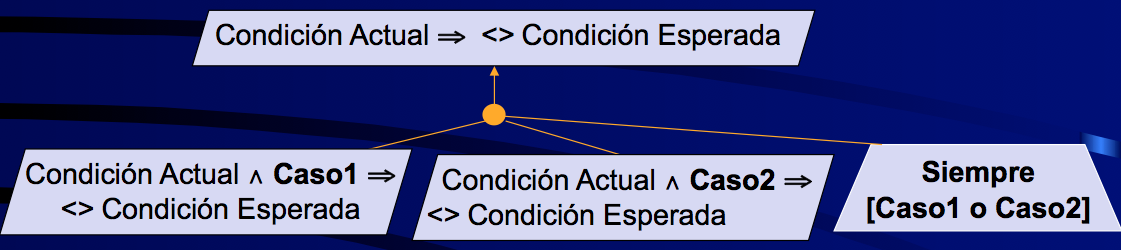
\includegraphics[scale=0.35]{Casos.png}
\end{center}

Entonces, como cuando vale en el Caso1 y vale cuando vale en el Caso2 (y la partición es completa) la conjunción de eso (pues es y-refinamiento) implica que vale en todos los casos. Al igual que el refinamiento por hitos, se puede generalizar a $n$ casos.

\subsubsubsection{Divide \& Conquer}
\begin{center}
	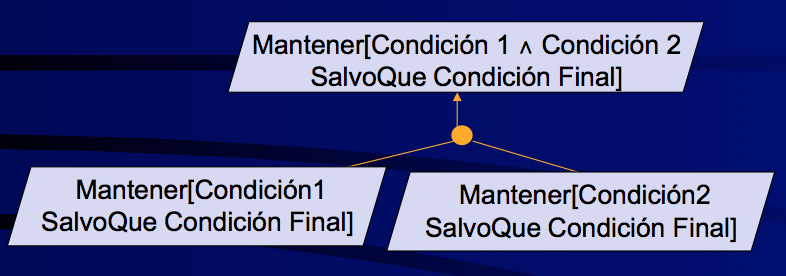
\includegraphics[scale=0.4]{DyC.png}
\end{center}

\subsubsubsection{Condiciones no monitoreables / no controlables}
En el caso de tener objetivos \textit{no realizables} por que involucran condiciones \textit{no monitoreables} o \textit{no controlables}, se puede aplicar una técnica para lograrlo. Sin embargo, para realizar esta técnica es necesario agregar una presunción de dominio específica, cosa que no siempre se puede hacer.

\begin{center}
	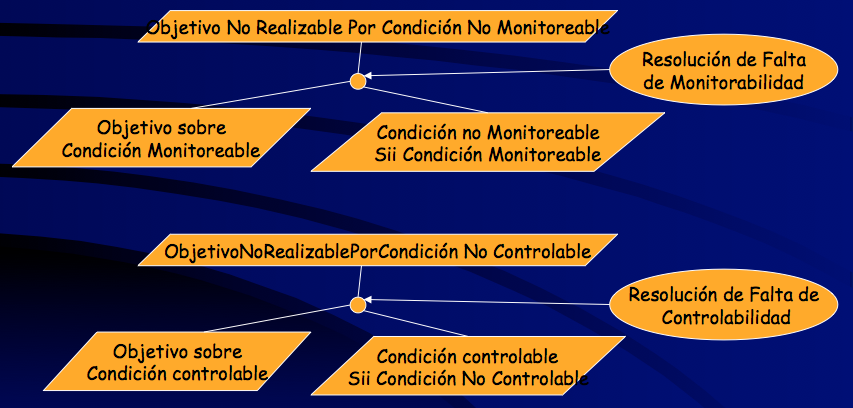
\includegraphics[scale=0.45]{CondNo.png}
\end{center}

\subsubsubsection{Análisis de Riesgo}
En un nodo de presunción de dominio $P$, puede aplicarse la técnica de \textbf{análisis de riesgo}. Esta técnica consiste en agregar un nodo con la negación de la presunción ($\neg P$) colgando de $P$ y refinar las condiciones que tienen que darse para que pase $\neg P$. A su vez se puede agregar (si se tuvieran) las probabilidades de que se de cada una de esas condiciones, pudiendo estimar fácilmente la probabilidad final de que ocurra el evento $\neg P$.

Otra mejora que se puede realizar a este modelo es agregar el costo de falla de la presunción, lo que nos permite directamente calcular la probabilidad de tener una pérdida si se diera $\neg P$ (nuevamente, tiene el problema de que esa información no siempre es accesible).

\subsubsection{Ventajas}
El modelo de objetivos presenta numerosas ventajas:
\begin{itemize}
	\item La técnica de refinamiento permite estructurar especificaciones.
	\item La estructura provee una justificación clara para los objetivos. Se establece un orden topológico en los objetivos.
	\item Simplifica mucho la tarea de detectar objetivos faltantes (\textbf{completitud}) y sobrantes (\textbf{pertinencia}).
	\item Permite plantear numerosas alternativas, documentando los pros y contras de cada una.
	\item Permite generar \textit{argumentos de satisfacción} (o sea, este objetivo lo podemos cumplir porque ya cumplimos todos sus hijos).
	\item Permite realizar análisis de riesgos, así como determinar el alcance del sistema.
\end{itemize}

\subsubsection{Objetivos}
La noción de objetivo puede ser extendida para aumentar la riqueza del diagrama y permitir que se grafique más información. Para esto, a los objetivos se los construye, no como hasta ahora, simplemente con una aserción prescriptiva, sino con:
\begin{itemize}
	\item \textbf{Tipo de objetivo}: describe el tipo del objetivo. Puede ser:
	\begin{itemize}
		\item \textit{Lograr}.
		\item \textit{Evitar}.
		\item \textit{Mantener}.
		\item \textit{Objetivo Blando}.
	\end{itemize}
	\item \textbf{Nombre}.
	\item \textbf{Categoría} (opcional): la partición en categorías de los objetivos puede emplearse como una heurística para elicitar requerimientos o analizar y reutilizar modelos. Permite establecer patrones de objetivos frecuentes.
	\item \textbf{Definición natural}: es la aserción prescriptiva, expresada en lenguaje natural.
	\item \textbf{Definición formal} (opcional): es la aserción prescriptiva, expresada en algún lenguaje formal (por ejemplo, lógica de primer orden, lógica proposicional, etc). Notar que no siempre es posible (o sencillo) expresar objetivos formalmente.
\end{itemize}

A su vez, también se pueden agregar otros atributos como \textit{referencia}, \textit{stakeholders afectados}, \textit{prioridad}, \textit{estabilidad}, \textit{costo}, etc.

\subsubsubsection{Clasificación}
Un objetivo se clasifica de \textbf{funcional} si es una función o servicio a ser provisto por el sistema. Deriva en una o más operaciones concretas en la interfaz.

A diferencia de esto, un objetivo \textbf{no funcional} es aquel que describe restricciones adicionales y no describe comportamiento específico del software. No dice \textit{qué} debe hacer el software sino por ejemplo \textit{cuán bien} o \textit{cuán rápido} lo debe hacer. En general no afectan a una operación concreta sino a grandes porciones de la funcionalidad (\textit{cross-cutting}).
~\newline

Ortogonalmente a esto, un objetivo se puede categorizar como \textbf{de comportamiento} o \textbf{blandos}. Un objetivo se dice de comportamiento cuando recorta el espacio de comportamiento permitido del software. La comprobación del objetivo es una función binaria que toma una traza o ejecución y devuelve si el objetivo se satisfizo. Para un sistema debo prohibir cualquier ejecución del mundo que no satisfaga alguno de mis objetivos. Los objetivos de comportamiento tienen un correlato con modelos operacionales de comportamiento (FSM y diagrama de secuencia). Son los de tipo \textit{lograr}, \textit{mantener} y \textit{evitar}.

Los objetivos blandos, en cambio son aquellos que denotan preferencia entre comportamientos. Permiten expresar ventajas y desventajas en cuanto a aspectos puntuales en o-refinamientos. Su satisfacción no puede establecerse mirando un sistema o una traza, deben compararse al menos dos. Es muy difícil vincular con modelos de comportamiento. Son los objetivos de tipo \textit{objetivo blando}. Pueden categorizarse en cosas del tipo \textit{maximizar}, \textit{incrementar}, \textit{mejorar}, etc. Existe una dualidad entre los objetivos blandos y las alternativas: los objetivos blandos pueden introducir alternativas nuevas, así como las ventajas/desventajas de una alternativa existente pueden introducir nuevos objetivos blandos.

Este tipo de objetivos tiene dos representaciones gráficas posibles:
\begin{itemize}
	\item Gráfica: nodos en el grafo del diagrama de objetivos. Cada nodo está asociado a al menos dos ejes de un o-refinamiento, especificando con `$+$' o `$-$' el orden relativo de las alternativas.
	\item Tabular: se grafican todos los objetivos blandos en una sola tabla. Las columnas representan los objetivos blandos mientras que las filas son las distintas alternativas. En la intersección entre una alternativa y un objetivo blando, se representa su ``medición'' (con `$+$' o `$-$').
\end{itemize}~\newline

Un objetivo se clasifica de \textbf{medible} si se puede medir. Idealmente, todos los objetivos deberían ser medibles. Los objetivos de comportamiento son trivialmente medibles (pues tienen la función de comprobación). Sin embargo, para los objetivos blandos, es necesario que haya un \textit{criterio de comparación} y para los de comportamiento debe haber un \textit{criterio de aceptación}.

Estas elecciones de criterios no siempre son triviales: puede haber objetivos para los cuales el concepto de medición sea difuso, que los \textit{stakeholders} no sean específicos, etc. Más aún, existe el problema de que generalmente, aún los objetivos que son medibles no los puede medir uno mismo; sólo los pueden medir los \textit{stakeholders}.

\subsubsubsection{Elicitación de objetivos}
El proceso de elicitación de objetivos puede realizarse \textbf{temprana-} o \textbf{tardía-} mente. En el primer caso, se indaga sobre los problemas y deficiencias del sistema actual (suponiendo que haya uno) y los objetivos de mejora y estrategia del cliente a futuro. Esto se puede realizar mediante distintas técnicas de elicitación, tales como \textit{basadas en stakeholders} (entrevistar stakeholders, tanto individual- como grupal- mente) o \textit{basadas en documentación} (revisar documentación del sistema existente). Es frecuente utilizar \textit{checklists de categorías} de objetivos.

En el caso de elicitación tardía (llamada elicitación \textbf{posterior}) se puede realizar por tres técnicas:
\begin{itemize}
	\item \textbf{Por abstracción} (bottom-up): se pregunta \textbf{``¿por qué?''} sobre distintos elementos (objetivos de bajo nivel, escenarios, descripciones operaciones, FSMs, manuales de procedimientos, etc). Por ejemplo, se indaga por algún objetivo puntual y conocido de bajo nivel (o conjunto de) y se pregunta ``¿Por qué se hace esto? ¿con qué fin?''. La respuesta a esto induce a descubrir uno o más objetivos a los que este objetivo contribuye, de nivel un poco más alto. Iterando este proceso, se puede ir planteando ``desde abajo hacia arriba'' un posible diagrama de objetivos. El alcance acota los objetivos. Se intenta relevancia de todos los fenómenos y propiedades en otros modelos. Se evita el riesgo de regresión de objetivos.
	\item \textbf{Por refinamiento} (top-down): se pregunta \textbf{``¿cómo?''} sobre objetivos disponibles. Similarmente al caso anterior, se indaga por algún objetivo pero de alto nivel y se pregunta: ``¿y cómo se logra esto? ¿hay otra opción?''. La respuesta permite plantear objetivos de más bajo nivel que contribuyan a lograrlo. Iterando, se puede plantear ``desde arriba hacia abajo'' un posible diagrama de objetivos. En general uno detiene el proceso cuando logra objetivos uni-agente (expectativas) o propiedades del entorno.
	\item \textbf{Por resolución de conflictos y obstáculos}: se plantea el diagrama a medida que van surgiendo conflictos, basándose en las soluciones planteadas.
\end{itemize}

\subsubsubsection{Objetivos vs Operaciones}
Es importante la distinción entre \textbf{objetivos} y \textbf{operaciones} / \textbf{casos de uso}. Las operaciones inducen objetivos mediante sus poscondiciones. Las operaciones podrían ser más generales. Pueden plantearse relaciones muchos a uno.


\subsubsubsection{Contra recíproco y complementario}
Frecuentemente, los objetivos del tipo \textit{lograr} tienen asociada una \textit{precondición} y una \textit{condición esperada}. O sea, son de la forma:
\begin{center}
	``Si \textit{precondición} entonces en el futuro \textit{condición esperada}''
\end{center}

De los objetivos de esta forma \underline{suelen} inducirse \textbf{objetivos de seguridad} \underline{relevantes} (no siempre ocurre que se puedan inducir y, cuando se puede, no siempre son relevantes). Estos objetivos son del tipo \textit{mantener}, se los llama \textbf{contra recíproco} y son de la forma:
\begin{center}
	``Siempre que \textit{condición esperada} entonces \textit{precondición}''
\end{center}~\newline

De los objetivos lograr de la antedicha forma también \underline{suelen} inducirse objetivos \underline{releavantes} llamados \textbf{complemento}, de la forma:
\begin{center}
	``Si \textbf{no} \textit{precondición} entonces $\hdots$''
\end{center}

\subsection{Modelo de operaciones}
%%NUEVO-COBY%%
Vimos el ``Diagrama de Casos de Uso''.
%%FIN-NUEVO-COBY%%

El \textbf{modelo de operaciones} es un modelo que permite \textbf{estructurar las operaciones}. Determina las operaciones o servicios que debe proveer la máquina y las transformaciones que deben ocurrir en el mundo como consecuencia de las antedichas operaciones.

Una \textbf{operación} se puede ver como una función que toma un estado del mundo y devuelve otro estado (una modificación de la entrada). Observar que \textbf{sólo pueden haber cambiado las variables controladas por la máquina}. Una operación es introducida por un objetivo uni-agente del modelo de objetivos (si son requerimientos introducen operaciones de software, si son expectativas inducen operaciones de agentes. No necesariamente uno a uno). Consta de:
\begin{itemize}
	\item \textbf{Operación}: nombre de la operación.
	\item \textbf{Responsable}: actor responsable de la operación.
	\item \textbf{Usuarios}.
	\item \textbf{Definición}: explicación de la operación.
	\item \textbf{Entrada}: la entrada que tomará la máquina para realizar la operación.
	\item \textbf{Salida}: la salida que devolverá la máquina después de realizar la operación sobre la entrada.
	\item \textbf{Pre-condición}: condiciones necesarias para que la operación pueda realizarse.
	\item \textbf{Post-condición}: condiciones cuya validez está garantizada después de la operación.
	\item \textbf{Trigger}: condición que si se da, la operación necesariamente ocurre.
\end{itemize}

\subsubsection{Diagrama de casos de uso}
Es una posible notación gráfica para el modelo de operaciones. Surge de la necesidad de estructurar las operaciones para facilitar su validación (caso contrario, la tarea se dificulta muchísimo por el enorme volumen de operaciones). El \textbf{diagrama de casos de uso} estructura el conjunto de operaciones atendiendo a la categoría de usuarios que participan en el mismo. Describen en forma de acciones y reacciones las operaciones provistas por la máquina desde el punto de vista del usuario (lo que facilita la validación por parte de los usuarios). Sólo se enfoca en la \textbf{funcionalidad} provista por la máquina a construir y la interacción máquina-agente, no busca dar una descripción detallada de funcionalidad.

Los diagramas de casos de uso sirven para definir claramente el alcance de la máquina a construir (lo que esté adentro de la caja) y facilitar la validación de funcionalidad con los \textit{stakeholders}.

Los diagramas de casos de uso constan de los siguientes	componentes:
\begin{itemize}
	\item \textbf{Actor}: se define como un conjunto de entidades concretas clasificados de acuerdo a una característica común a ellos. Representa a un tipo de usuario, abstrayendo al usuario real (que puede ser personas, sistemas, dispositivos, softwares, máquinas, etc). El nombre del actor describe su rol desempeñado. Si bien no es uno a uno, existe una correlación entre los agentes y los actores del modelo de objetivos (un agente puede estar modelado por varios actores, sea simultáneamente, alternadamente o algo así).
	\item \textbf{Máquina}: se representa con un rectángulo. Dentro de ella viven los casos de uso que se llevan a cabo dentro de ella.
	\item \textbf{Caso de uso}: especifica una o más secuencias de acciones que el sistema puede llevar a cabo interactuando con sus actores. Describe un conjunto de escenarios. Su nombre suele expresarse en gerundio. Consideremos una ejecución como un conjunto de tuplas \textbf{(a,o,a')}, que debe interpretarse como que el actor $a$ ejecuta la operación $o$ sobre el actor $a'$. Entonces un caso de uso puede verse como un conjunto de estas secuencias que verifica que antes de la primer tupla vale la precondición y después de la última vale la postcondición.
\end{itemize}

En muchas ocasiones, un nombre en gerundio no alcanza para especificar un caso de uso (por ejemplo, para explicar una interacción crítica, o clasificar aspectos de la funcionalidad o roles de los actores). Existen numerosas formas de subsanar esta carencia, siempre generando una \textbf{descripción detallada de casos de uso}. Esta descripción, puede realizarse en lenguaje formal, informal, secuencia de operaciones, tablas, diagramas de secuencia, máquinas de estado, etc. Es decir, es extremadamente versátil la forma de documentar detalladamente un caso de uso, aunque suele ser buena práctica agregar pre y post condiciones.

Sea cual sea la forma de detallar los casos de uso que se elija, es habitual que durante la ejecución de un caso de uso aparezcan \textbf{errores} o \textbf{excepciones} en los cuales se suele desviar el curso normal del programa. A esta desviación se la llama \textbf{alternativa}. Es importante que el detalle de caso de uso explicite estas alternativas.

En estos detalles de casos de uso, frecuentemente se explicitan las circunstancias en las que un caso de uso ``usa'' a otro. Estas ``llamadas'' denominan \textbf{punto de uso}.

\subsubsubsection{Relaciones}
Dado que el diagrama de casos de uso se usa muy informalmente, se introducen las relaciones entre casos de uso para proveer un poco de estructura y establecer relaciones entre los distintos elementos del diagrama. Algunas de estas relaciones son:

\begin{itemize}
	\item \textbf{Participa en}: un actor $A$ \textit{participa en} un caso de uso $U$ si y sólo si la descripción detallada de $U$ hace referencia \underline{explícita} al actor $A$ como participante de la interacción. Es una notación \underline{sintáctica}. Observar que que $A$ participe en $U$ no garantiza que en todo escenario $s \subseteq U$, $A$ interactúe con el sistema en $s$ (por ejemplo, podría no ocurrir en una alternativa).

	\begin{center}
		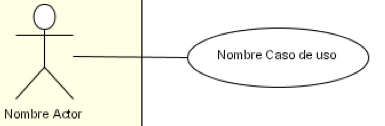
\includegraphics[scale=0.5]{Partic.png}
	\end{center}

	\item \textbf{Herencia}: semánticamente, $X$ \textit{hereda de} $Y$ si y sólo si $X \subseteq Y$. Se utiliza para estructurar actores según la relación ``es un tipo especial de''. Si un actor $a'$ \textit{hereda de} un actor $a$ (se nota con $a' \rightarrow a$) entonces todos los casos de uso que son relevantes para $a$, lo son para $a'$, pero no vale la vuelta.

	Si $Y$ tiene especializaciones $x_1,...,x_n$ y vale que $\forall y\in Y, y\in x_i$ para algún $1\leq i\leq n$, entonces $Y$ se denomina \textbf{abstracto}. O sea una entidad es abstracta sólo si todos sus elementos pertenecen a alguna de sus especializaciones. Se utilizan para estructurar más cómodamente e introducir conceptos relevantes.

	\begin{center}
		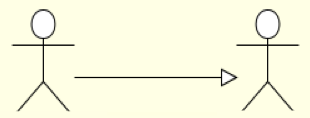
\includegraphics[scale=0.5]{Heren.png}
	\end{center}

	\item \textbf{Inclusión}: un caso de uso $A$ \textit{incluye a} un caso de uso $B$ si y sólo si cuando un escenario $s$ es descripto por $A$, entonces existe una porción de $s$ que contiene un escenario descripto por $B$.

	\begin{center}
		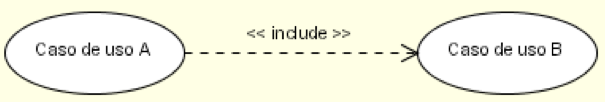
\includegraphics[scale=0.5]{Inclus.png}
	\end{center}

	\item \textbf{Extensión}: un caso de uso $A$ \textit{extiende a} un caso de uso $B$ si y sólo si existe un escenario $s$ denotado por $A$, que contiene un escenario denotado por $B$ (pueden haber escenarios denotados por $B$ que no aparezcan en escenarios denotados por $A$). Representan una parte de la funcionalidad del caso que no siempre ocurre. Suelen utilizarse para errores, excepciones y casos alternativos.

	\begin{center}
		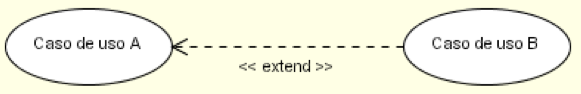
\includegraphics[scale=0.5]{Extens.png}
	\end{center}
\end{itemize}

\subsubsubsection{Super-Actores y Casos de uso auxiliares}
Un \textbf{super-actor} es un actor abstracto, agregado con el sólo propósito de tipar un caso de uso incluido en muchos otros. Para que no ensucie la notación, es importante que sea realmente relevante desde el punto de vista del problema.

Es frecuente en lenguajes formales sea necesario introducir elementos poco intuitivos para saltear las restricciones sintácticas del lenguaje. Si bien en ocasiones es imposible eludir el uso de  este tipo de construcciones, es buena práctica intentar evitarlas. Para esto, los diagramas de actividad permiten agregar casos de uso \textbf{auxiliares}. Estos casos de uso no agregan expresividad al lenguaje, pero sí permiten ordenar y aclarar, resumiendo cosas ya dichas. Sirven para evitar introducir \textbf{elementos foráneos} en el diagrama de casos de uso.

Así, un caso de uso $U$ es auxiliar si:
\begin{itemize}
	\item En el diagrama, no hay actores que participen en él (prohibido en la cátedra de IngSoft 1).
	\item Las referencias a actores en la descripción detallada de $U$ son de un tipo de actor abstracto $A$ definido implícitamente.
	\item El actor abstracto $A$ es super-actor de todos los actores que participan de casos de uso que usan a $U$ y todos los casos de uso que son extendidos por $U$.
\end{itemize}

\subsubsection{Relación con los otros modelos}
\begin{itemize}
	\item \textbf{Modelo de Jackson}: fenómenos en la interfaz vs operaciones.
	\item \textbf{Modelo de agentes}: consistencia agentes y actores: interfaz, visibilidad de fenómenos.
	\item \textbf{Modelo de las 4 variables}:monitorabilidad / controlabilidad vs. Agente responsable / entrada / salida.
	\item \textbf{Modelo de Objetivos}: relación muchos a muchos entre requerimientos y expectativas vs. operaciones
\end{itemize}

\subsection{Modelo Conceptual}
%%NUEVO-COBY%%
Vimos el ``Diagrama de Clases''.
%%FIN-NUEVO-COBY%%

También conocido como ``modelo de dominio'', es el modelo más clásico de la ingeniería de requerimientos. Intenta explicar y estructurar la definición de los \textbf{conceptos} relevantes (en la definición del problema) de tal forma que sea validable. Los conceptos son los sustantivos asociados al dominio del problema.

Para su representación existen diversas técnicas, con distintos niveles de complejidad:
\begin{itemize}
	\item \textbf{Diccionario / Glosario}: es una lista de clases con sus atributos y relaciones. Tiene poca estructura y es complicado de analizar/validar. Se usa lenguaje natural para explicar la denotación en detalle.
	\item \textbf{Diagrama de Entidad-Relación (DER)}: usa un lenguaje gráfico que provee estructura. Muy usado para bases de datos.
	\item \textbf{Diagrama de clases}: extiende DER con varias características, como \textit{herencia}, \textit{modificadores}, etc.
\end{itemize}

\subsubsection{Definiciones}
\begin{itemize}
	\item \textbf{Objeto conceptual}: denota una entidad o concepto del dominio del problema. Puede ser un \textit{objeto pasivo}, \textit{objeto activo}, \textit{personas}, \textit{estructuras}, etc.
	\item \textbf{Clase conceptual}: denota un conjunto de objetos conceptuales que comparten características comunes. Estas características pueden ser:
	\begin{itemize}
		\item \textbf{Atributo}: es una característica intrínseca al objeto, completamente independiente de otros objetos. Consta de un nombre y, posiblemente, un rango.
		\item \textbf{Relación}: es una característica que vincula conceptualmente un objeto a otros. Cada objeto juega un rol conceptual en ese vínculo.
	\end{itemize}
	Para identificar clases conceptuales se utilizan estrategias tales como: \textit{identificar frases nominales}\footnote{Frase nominal: sustantivo o conjunto de palabras que actúan como tal.} \textit{en la descripción de dominio} o \textit{utilizar listas de categorías de clases conceptuales}.

	Expresan “tipos” de entidades conceptuales del mundo real.
\end{itemize}

\subsubsection{Categorías de clases conceptuales}
\begin{multicols}{2}
	\begin{itemize}
		\item Objetos tangibles o físicos.
		\item Especificaciones, diseños o descripciones.
		\item Lugares.
		\item Transacciones.
		\item Líneas de la transacción.
		\item Roles de gente.
		\item Contenedores de otras cosas.
		\item Contenidos.
		\item Otros sistemas informáticos o electromecánicos externos al sistema.
		\item Conceptos abstractos.
		\item Organizaciones.
		\item Hechos.
		\item Procesos (no frecuente).
		\item Reglas y políticas.
		\item Catálogos.
		\item Registros de finanzas, trabajos, contratos, etc.
		\item Instrumentos y servicios financieros.
		\item Manuales, documentos, artículos de referencia, libros.
		\item Relaciones.
	\end{itemize}
\end{multicols}

\subsubsection{Diagrama de clases}
En los diagramas de clases se emplea una notación gráfica particular para denotar las clases conceptuales, sus atributos y sus relaciones.

Las clases conceptuales se denotan con un rectángulo cuyo título es el nombre de la clase y, abajo, se listan sus atributos. Las relaciones entre clases conceptuales se notan con líneas uniendo los distintos rectángulos, sobre las que se escriben las características de la relación (nombre y cantidad).

Junto con los diagramas de objetos, los diagramas de clases se usan para modelar el dominio del problema y el de la solución.

\begin{center}
	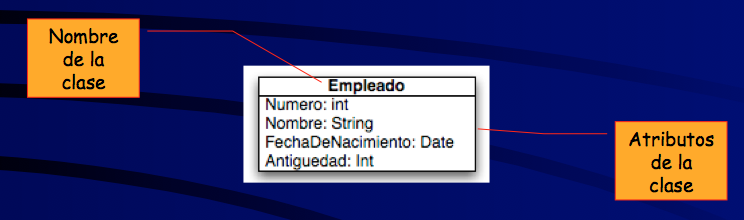
\includegraphics[scale=0.5]{Conceptual.png}
\end{center}

\subsubsubsection{Asociaciones entre clases}
Una \textbf{asociación} entre dos clases expresa una conexión bidireccional entre objetos. Es una abstracción de la relación existente en los enlaces entre objetos. Para agregar restricciones sobre las asociaciones y enlaces se agregan elementos de \textbf{multiplicidad}: en la asociación, se especifican cotas inferiores y superiores para la cantidad de instancias de las clases que se relacionan por esa asociación. A su vez, para simplificar la lectura de los vínculos se emplean \textbf{roles}: se asigna un nombre al final de la asociación, que explica la relación entre los conceptos en un sentido particular. Cada asociación tiene dos roles que permiten navegar la asociación en ambos sentidos.

\begin{center}
	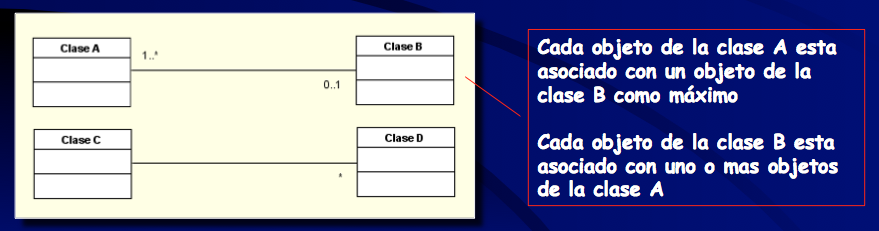
\includegraphics[scale=0.5]{Asociacion.png}
\end{center}

\subsubsubsection{Agregación}
Es un tipo de asociación especial, del tipo ``parte de / todo'' dentro de la cual una o más clases son parte de un conjunto. Se indica con un rombo. Indica cuándo un objeto de una clase (que es un todo, un objeto indivisible) se piensa como parte de otro objeto de otra clase.

\begin{center}
	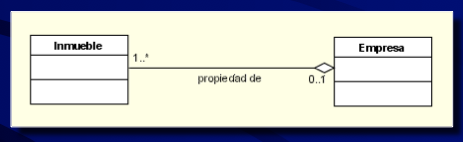
\includegraphics[scale=0.6]{Agregacion.png}
\end{center}

\subsubsubsection{Composición}
Es una forma fuerte de agregación que denota que un objeto de una clase es parte de un objeto de otra. Si no forma parte de tal objeto, entonces carece de sentido. Se diferencia de la agregación normal en que:
\begin{itemize}
	\item En la composición tanto el todo como las partes tienen el mismo ciclo de vida.
	\item Un objeto puede pertenecer solamente a una composición.
\end{itemize}

\begin{center}
	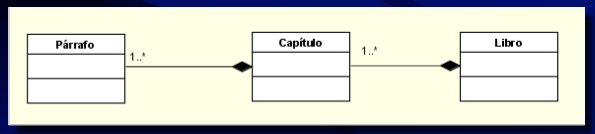
\includegraphics[scale=0.6]{Composicion.png}
\end{center}

\subsubsubsection{Asociación calificada}
Es un azúcar sintáctico que permite representar muchas asociaciones en forma compacta. Se utiliza un \textbf{calificador}: un atributo (o tupla de atributos) de la asociación cuyos valores sirven para particionar el conjunto de objetos enlazados a otro (observar que el rectángulo calificador es parte de la \underline{asociación} y no de la clase).

\begin{center}
	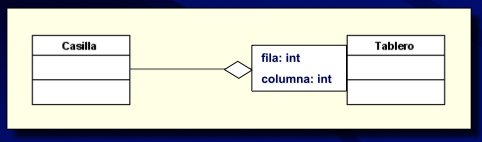
\includegraphics[scale=0.6]{AsoCalificada.png}
\end{center}

\subsubsubsection{Asociaciones $n$-arias}
Son asociaciones que se establecen entre más de dos clases. Una clase puede aparecer varias veces desempeñando distintos roles. Semánticamente, son una forma de aplicar restricciones y explicitar relaciones entre $n$ clases de equivalencia. Pueden ser usadas para refinar un modelo. La multiplicidad en las clases $n$-arias suele ser difícil de definir. Generalmente se refieren a una clase contra todas las demás (o se aclara en lenguaje natural a cuál se refiere).

\begin{center}
	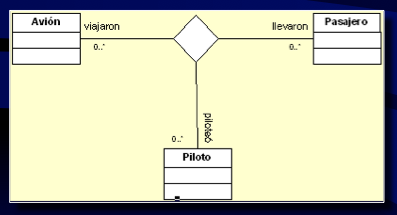
\includegraphics[scale=0.6]{Narias.png}
\end{center}

\subsubsubsection{Generalización o Herencia}
Es una relación entre una clase general (superclase o padre) y una versión más específica de dicha clase (subclase o hija). El hijo hereda todos las características y atributos del padre (aunque pueden incluir atributos o relaciones que el padre no tiene). A la hora de realizar una interpretación, la herencia denota \textbf{inclusión de instancias}: todo objeto de la clase hija es a su vez un objeto de la clase padre.

Se extiende la herencia con los siguientes modificadores:
\begin{itemize}
	\item \textbf{Overlapping/Disjoint}.
	\item \textbf{Complete/Incomplete}.
\end{itemize}

Observar que una clase puede generalizar a dos conjuntos de hijos distintos. Se utiliza una anotación (llamada \textbf{discriminador}) para documentar la distinta intención que cada clasificación tiene.

También puede extenderse con \textbf{herencia múltiple} en el cual la clase hijo es la intersección de dos clases padre.

%Dos padres y un hijo. Corregir.

\begin{center}
	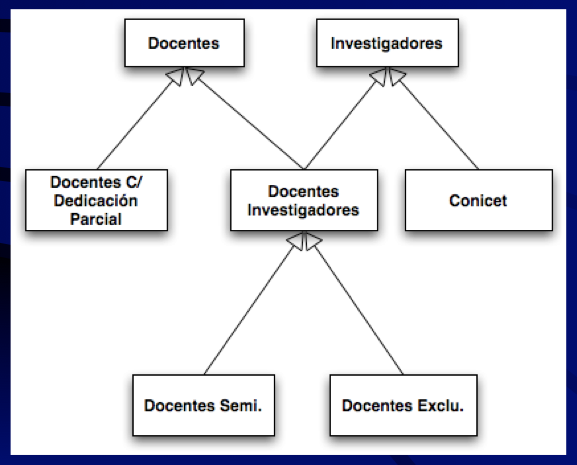
\includegraphics[scale=0.5]{Herencia.png}
\end{center}

\subsubsubsection{Clases de asociación}
Las clases de asociación modelan características de una asociación que son independientes de las clases que asocian. Informalmente, es una clase que no tiene sentido por sí sola. Si algo cambia en la clase es porque alguna de las clases que involucra cambió.

Formalmente, si $C$ es una clase de asociación para $R$ en $A$x$B$, entonces introduce una función $f:R\rightarrow C$. Se garantiza que
\begin{itemize}
	\item Para un mismo par $(a,b)$ no existe más de un $c$.
	\item Para todo $c$ en $C$ existe $r$ tal que $f(r)=c$.
	\item Si $c=f(r)$, $c$ no puede cambiar por sí sola (si cambia es porque la naturaleza de la asociación cambió).
\end{itemize}

\begin{center}
	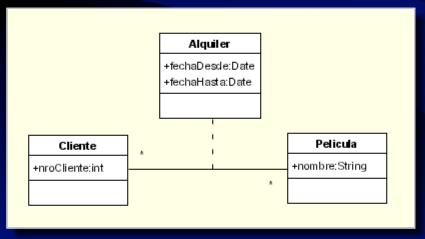
\includegraphics[scale=0.6]{ClaseAsociacion.png}
\end{center}

\subsubsubsection{Otros}
Existen muchos otros modificadores y elementos sintácticos que pueden ser usados en los diagramas de clases. Algunos muy usados son:
\begin{itemize}
	\item \textbf{Clases enumeradas}: conjuntos de valores prefijados.
	\item \textbf{OR / XOR de relaciones}.
	\item \textbf{Subset}.
	\item \textbf{Atributos derivados}: explicitan invariantes.
\end{itemize}

\subsubsubsection{Diagrama de Objetos}~\newline
 \indent Informalmente, se puede ver como una instanciación a un momento determinado de un diagrama de clases: define el mundo en un instante dado. La relación entre dos objetos se corresponde con la de sus clases (toda instancia de una clase $X$ tiene enlaces con instancias de $Y$ de acuerdo al tipo de relación, atributos y modificadores que $X$ tiene con $Y$ en el modelo de clases).

En este contexto, un \textbf{objeto} denota una entidad conceptual del mundo real.

\begin{center}
	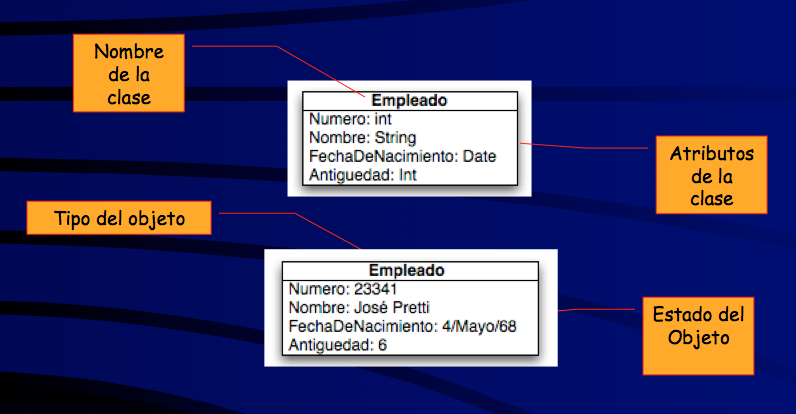
\includegraphics[scale=0.45]{DiagObjetos.png}
\end{center}


\subsubsection{Modelo conceptual vs Diseño}
A diferencia de esto, en el modelo de diseño las clases y objetos discriminen cómo se agrupará el \emph{código} (no conceptos) y los datos al momento de programar el software y al momento de ejecutarlo. A su vez, las operaciones son frecuentemente asignadas a objetos y clases (en el modelo conceptual esto sólo tiene sentido para \textbf{entidades activas}).

\subsubsection{Relación con los otros modelos}
\begin{itemize}
	\item \textbf{Modelo de objetivos}: describe la estructura estática del mundo sobre la que los objetivos predican. Es la base para formalizar objetivos.
	\item \textbf{Modelo de agentes}: no existe una correspondencia uno a uno entre agentes y clases. Los diagramas de contexto describen el estado interno de los agentes y las operaciones que provee.
\end{itemize}

\subsection{OCL}
El \textbf{OCL} (\textit{Object Constraint Language}) es un lenguaje formal que permite definir restricciones sobre objetos. Observar que no es un modelo en sí mismo, sino una herramienta para ser utilizada con otros modelos:
\begin{itemize}
	\item \textbf{Modelo conceptual}.
	\item \textbf{Modelo de operaciones}: se utiliza para definir formalmente las condiciones (\textit{pre}, \textit{post} y \textit{trigger}).
	\item \textbf{Modelo de objetivos}: si bien es necesario dotarlo de operadores temporales, se puede utilizar para generar una definición formal de objetivos.
	\item \textbf{Diseño}: es utilizado para formalizar contratos y aumentar la expresividad de los diagramas de clases.
	\item \textbf{Navegación de modelos estructurales}.
\end{itemize}

\subsubsection{OCL en modelo conceptual}
Se utiliza para agregar restricciones adicionales a los diagramas de clases. Estas restricciones en general tienen un carácter complejo que redunda en que no puedan ser expresada por la acotada e inexpresiva sintaxis de los antedichos diagramas. Las restricciones ayudan a definir qué es un estado \underline{válido} en el contexto del modelo.

El vocabulario de OCL es dependiente del modelo conceptual sobre el que se esté aplicando (o sea, el modelo conceptual introduce una signatura para las aserciones OCL).

Las aserciones en OCL usado en modelo conceptual siguen la siguiente estructura:
\begin{center}
	\fbox{\textbf{Context} \textit{contexto} \textbf{inv}: \textit{invariante}}
\end{center}
donde

\begin{itemize}
	\item \textit{contexto}: define \textit{en dónde} se espera que la aserción sea verdadera.
	\item \textit{invariante}: define la aserción misma.
\end{itemize}

\subsubsubsection{Semántica}
Semánticamente, una descripción de modelo conceptual usando OCL está dada en los mismos términos que una descripción de modelo conceptual: conjuntos de objetos con atributos y las relaciones entre sí. La diferencia es que el OCL es notablemente más expresivo, con lo que podemos \textbf{recortar} modelos inválidos con más precisión.

\subsubsubsection{Recorte o Prunning}
La semántica de \textbf{recorte} o \textbf{prunning} define que a medida que agregamos restricciones y especificaciones el espacio de interpretaciones \underline{válidas} se va achicando (justamente, lo estamos recortando). Tanto el modelo de operaciones (con pre- y post-condiciones) como el de objetivos (mediante objetivos de comportamiento que deban cumplirse) utilizan semántica de prunning.

\begin{center}
	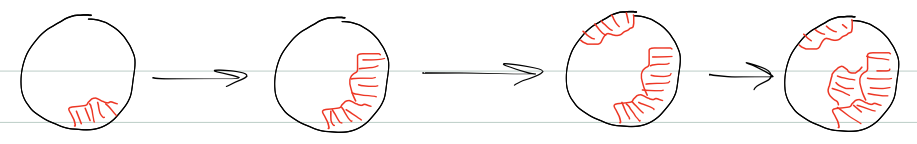
\includegraphics[scale=0.5]{Prunning.png}
\end{center}

\subsubsubsection{Sintaxis}
La sintaxis de OCL se define recursivamente a partir del modelo conceptual sobre el que se aplica. Cada clase conceptual introduce un \textbf{tipo} en el lenguaje. \textbf{Self} indica el objeto actual.

Las expresiones se construyen a partir de:
\begin{itemize}
	\item \textbf{Constantes}: Ej. ``5''
	\item \textbf{Variables tipadas}: Ej. ``Estudiante''
	\item \textbf{Queries}: funciones sin efectos colaterales para especificaciones más concisas.
	\item \textbf{Atributos}: Ej. ``Estudiante.nombre''
	\item \textbf{Roles}: Ej. ``Estudiante.materias$\_$aprobadas''
	\item \textbf{Tipos predefinidos y sus operaciones}: Ej. \textit{tipos básicos}, \textit{comparadores $<$, $>$, $=$}, \textit{bag}, \textit{set}, etc.
\end{itemize}

~\newline

El lenguaje de OCL viene con tipos \textbf{paramétricos} predefinidos para modelizar \textbf{colecciones} de objetos. Algunos de estos son:
\begin{itemize}
	\item \textbf{Collection}($T$): colección genérica de elementos de tipo $T$.
	\item \textbf{Set}($T$): colección \textit{no ordenada} y \textit{sin repetidos} de elementos de tipo $T$.
	\item \textbf{OrderedSet}($T$): colección \textit{ordenada} y \textit{sin repetidos} de elementos de tipo $T$.
	\item \textbf{Bag}($T$): colección \textit{no ordenada} y \textit{con repetidos} de elementos de tipo $T$.
	\item \textbf{Sequence}($T$): colección \textit{ordenada} y \textit{con repetidos} de elementos de tipo $T$.
\end{itemize}

Estos tipos a su vez vienen con operaciones asociadas. Por ejemplo, supongamos que $X$ e $Y$ son dos instancias del tipo \textit{collection($T$)}, $t$ de tipo $T$ y $P(t)$ un predicado $P(t):T\rightarrow Bool$. En ese caso, son válidas las operaciones:
\begin{itemize}
	\item $X\rightarrow$ size()
	\item $X\rightarrow$ intersection($Y$) , $X\rightarrow$ union($Y$)
	\item $X\rightarrow$ isEmpty() , $X\rightarrow$ notEmpty()
	\item $X\rightarrow$ includes($t$) , $X\rightarrow$ excludes($t$)
	\item $X\rightarrow$ includesAll($Y$) , $X\rightarrow$ excludesAll($Y$)
	\item $X\rightarrow$ collect($P(t)$) , $X\rightarrow$ select($P(t)$) , $X\rightarrow$ reject($P(t)$) , $X\rightarrow$ forAll($P(t)$)
\end{itemize}

\textit{Set}, \textit{orderedSet}, \textit{bag} y \textit{sequence} son subtipos de \textit{collection} (o sea, heredan todas son operaciones), pero agregan algunas propias de cada uno. Por ejemplo,
\begin{itemize}
	\item \textit{Bag} agrega $X\rightarrow$ count($t$)
	\item \textit{OrderedSet} y \textit{sequence} agregan $X\rightarrow$ first() y $X\rightarrow$ last()
\end{itemize}

La navegación por roles permite recorrer el diagrama de clases a través de las asociaciones de una determinada clase. Eso es extremadamente útil para imponer restricciones: en el lenguaje OCL \textit{$<$clase$>$.$<$rol$>$} retorna la \textbf{colección} de objetos que están del otro lado de la asociación. Si tiene multiplicidad 1, retorna sólo el objeto (y no la colección).

Esto induce un problema de tipos. No siempre es posible inducir sólo con mirar el diagrama de clases el tipo de expresión. \textit{$<$Clase$>$.$<$rol$>$} puede ser una colección o un objeto en sí mismo. Para solucionar esto, se introducen dos conceptos: el \textbf{tipo aparente} de una expresión es el que se puede deducir \textbf{estáticamente} de la signatura del diagrama de clases. A diferencia de esto, el \textbf{tipo real} debe deducirse \textbf{dinámicamente} del objeto mismo.  Para esto, el lenguaje OCL incluye funciones que permiten realizar esta deducción de tipos dinámica.
\begin{itemize}
	\item $x.oclIsKindOf(t)$ devuelve \textit{true} si el tipo real de $x$ es subtipo de $t$.
	\item $x.oclIsTypeOf(t)$ devuelve \textit{true} si el tipo real de $x$ es $t$.
	\item $x.oclAsType(t)$ devuelve una referencia denotando lo mismo que $x$, pero casteado\footnote{Casting: proceso de cambiarle el tipo aparente a una variable en OCL.} con tipo aparente $t$.
\end{itemize}

\subsubsubsection{Reglas de subtipificación}
Definimos la relación $<$ de la siguiente manera: \textit{sean $T_1$ y $T_2$ tipos correspondientes a clases $T_1$ y $T_2$. Vale que $T_1<T_2$ si y sólo si $T_1$ es \textbf{subclase} de $T_2$}. Entonces, para toda expresión de tipo $T$, vale que:
\begin{itemize}
	\item \textit{set($T$)} $<$ \textit{collection($T$)}
	\item \textit{sequence($T$)} $<$ \textit{collection($T$)}
	\item \textit{Bag($T$)} $<$ \textit{collection($T$)}
	\item $T <$ \textit{OclAny}
	\item Si $T_1 < T_2$ y $C$ es \textit{collection}, \textit{set}, \textit{bag} o \textit{sequence}, entonces $C(T1) < C(T2)$. %Consulta OCL Synthax semanthics and tools
\end{itemize}

\subsubsubsection{Queries}
Las \textbf{queries} son funciones sin efectos colaterales, usadas en el modelo conceptual para especificaciones muy concisas. Son definiciones auxiliares que no van en el diagrama de clases. Las clases conceptuales no proveen queries.

\subsubsection{OCL fuera de modelo conceptual}
OCL no es muy utilizado fuera del modelo conceptual (especialmente en esta materia). Sin embargo, existen otros usos, tales como:
\begin{itemize}
	\item \textbf{Modelo de operaciones}: puede utilizarse para definir pre- y post- condiciones de operaciones o casos de uso. Se utiliza el operador \textbf{@pre}. Puede ser el lenguaje utilizado para formalizar operaciones provistas por la máquina y otros agentes.
	\item \textbf{Diseño}: puede utilizarse para definir pre- y post- condiciones de operaciones o casos de uso. Se utiliza el operador \textbf{@pre}.
	\item \textbf{Modelo de objetivos}: puede utilizarse para formalizar objetivos.
\end{itemize}

\subsection{Modelos de Comportamientos}
%%NUEVO-COBY%%
Vimos el ``Diagrama de Actividad'' y FSMs.
%%FIN-NUEVO-COBY%%

En los \textbf{modelos de comportamientos} se estudian las reacciones y respuestas de un agente cuando es estimulado. Llamamos \textbf{modelos de comportamiento} a una familia de notaciones que describen comportamiento.

Formalmente, se define \textbf{comportamiento} como \textit{el conjunto de respuestas o reacciones o movimientos hechos por un organismo en cualquier situación}. Para representar eso, se emplean cadenas de estímulos y respuestas con una determinada sintaxis y semántica. Estas cadenas se realizan una para cada agente. Para verificar si el sistema logra sus objetivos, se debe verificar la \textbf{composición} de toda cadena de estímulos y respuestas del conjunto de agentes.

Los modelos de comportamiento tienen una semántica \textbf{generativa} (induce una forma de generar lo que se concibe) o \textbf{ejecutable}. Contrariamente al \textit{prunning}, al agregar elementos se expande el conjunto de ejecuciones válidas del sistema.

Se categorizan en dos:
\begin{itemize}
	\item \textbf{Basados en estados}: es una visión centrada en un agente en particular. Selecciono un agente y describo todas sus posibles interacciones con cualquier otro agente. Tienen como foco describir la interacción entre varias
entidades. Su objetivo es ejemplificar interacciones importantes. No hay, como en los modelos basados en estados una visión sesgada a un sólo agente, sino que se considera una sola \textbf{traza} gobal, omnisciente.

	\item \textbf{Basados en interacciones}: es una visión de traza global (visión omnisciente) en la que selecciono un conjunto de agentes y describo todas las posibles interacciones entre sí. No ``se para'' en ningún agente en particular. Su foco está en describir cómo es la interacción entre varias entidades.
\end{itemize}

\subsubsection{Diagramas de Secuencia}
Son una de las posibles herramientas \textbf{basada en interacciones} para representar gráficamente y trabajar con modelos basados en interacciones. Provienen de las Telco. Su scope permite describir escenarios de intercambios de mensajes estableciendo posibles ordenamientos para los eventos. Poseen una semántica de órdenes parciales. Se componen por intermedio de un grafo.

\begin{center}
	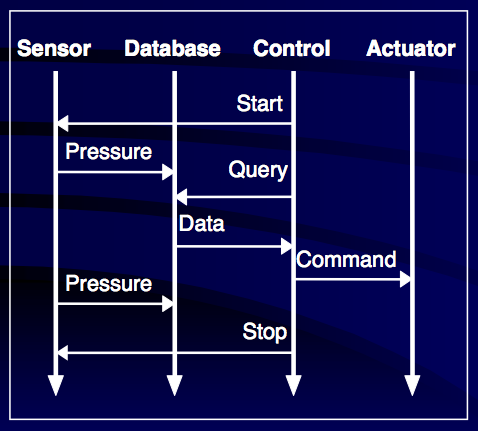
\includegraphics[scale=0.5]{DiagSeq.png}
\end{center}

Las líneas verticales pueden representar agentes (dependiendo de para qué se esté usando el diagrama) y las horizontales representan \textbf{comunicación sincrónica} entre ellos. También se puede representar comunicación \textbf{asincrónica}, en cuyo caso el orden parcial es de eventos de envío y recepción.

\subsubsubsection{HMSCs: High-Level Message Sequence Chart}
Un HMSC es una descripción gráfica de la relación entre MSCs. Establece un orden topológico entre las MSCs, permitiendo cosas como loops condicionales, etc. La forma de reconstruir el comportamiento de la máquina es realizando una \textbf{composición secuencial débil}. Pueden usarse con semántica de comunicación asincrónica.

%%NUEVO-COBY%%
\underline{Sincrónico:} dícese de un fenómeno que ocurre en perfecta correspondencia temporal con otro evento o proceso.
%%FIN-NUEVO-COBY%%

\begin{center}
	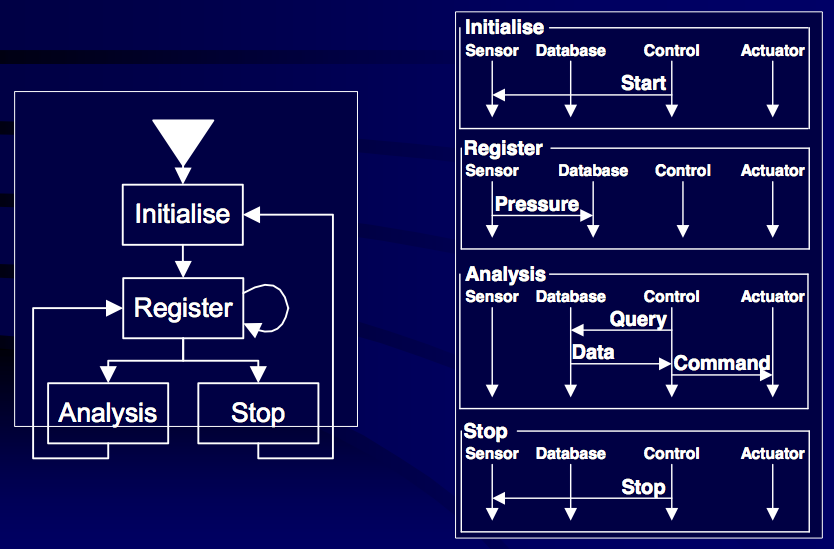
\includegraphics[scale=0.5]{hMSC.png}
\end{center}

Su nivel de expresividad es relativamente limitado, porque no pueden expresar a todos los lenguajes regulares (por ejemplo, hay protocolos de estados finitos que no se pueden describir mediante HMSCs). Sin embargo, existen algunos lenguajes no-regulares que sí pueden ser expresados. \textit{Temporal Model Checking} no es decidible.

Un ejemplo de una \textit{HSMC} de lenguaje no regular (aún considerando comunicación sincrónica) es:
\begin{center}
	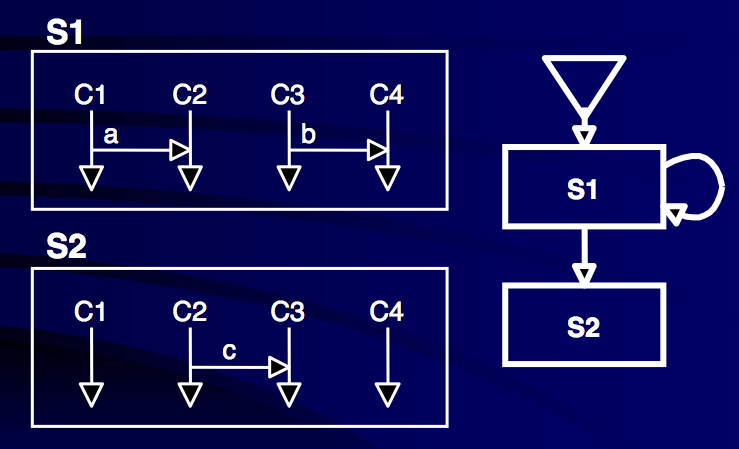
\includegraphics[scale=0.5]{hmscnoreg.png}
\end{center}

%\textbf{PREGUNTAR ESTO (????)}

No todo puede ser representado mediante una \textit{HMSC}. Por ejemplo, los \textbf{protocolos de estados finitos}.

Aún si suponemos comunicación sincrónica y una \textit{HMSC} que genera un lenguaje regular \textbf{no necesariamente} podemos armar un sistema que implementa exactamente el comportamiento especificado. Esto se puede ver en que puede generarse un \textbf{escenario implicado}.

\subsubsubsection{De interaction-based a state-based}
Un \textit{MSC} (\textit{Message Sequence Chart}) dado tiene dos interpretaciones semánticas: se pueden extraer tanto las \textbf{trazas del sistema} como las \textbf{estructuras e interfaces} de los que el sistema se vale. Pasado a un plano de \textbf{state-based modelling}, puede construirse una \textbf{FSM (Finite State Machine)} basándose en cada una de las \textit{MSCs}. A este proceso se lo llama \textbf{síntesis}. Sin embargo, vale preguntarse si esta \textit{FSM} resultante preserva la arquitectura (o sea, las estructuras e interfaces se mantienen coherentes con los \textit{MSCs} del modelo basado en interacción) y si respeta las trazas del sistema (o sea, si existe una equivalencia entre las trazas del sistema extraídas de las \textit{MSCs} y las de la \textit{FSM}).

\begin{center}
	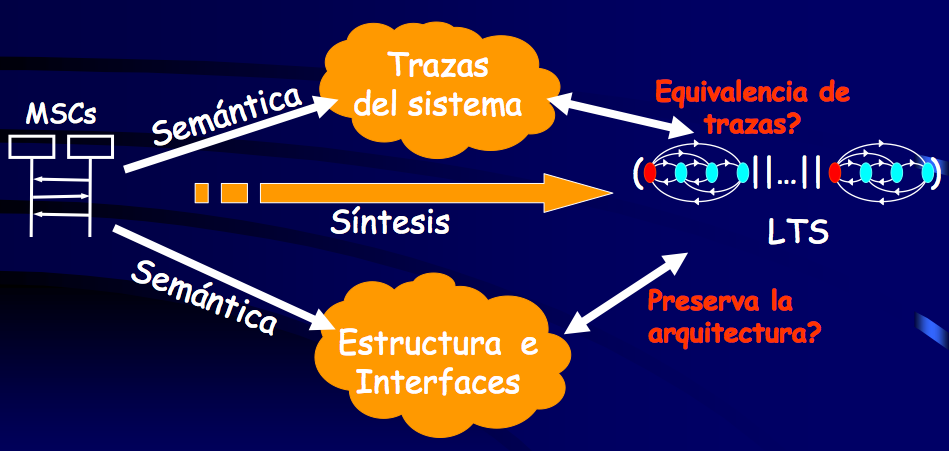
\includegraphics[scale=0.45]{InterState.png}
\end{center}

El llamado problema de la síntesis plantea que no siempre es posible observando las trazas del sistema sintetizar los componentes individuales. Por ejemplo, supongamos el siguiente caso:

\begin{center}
	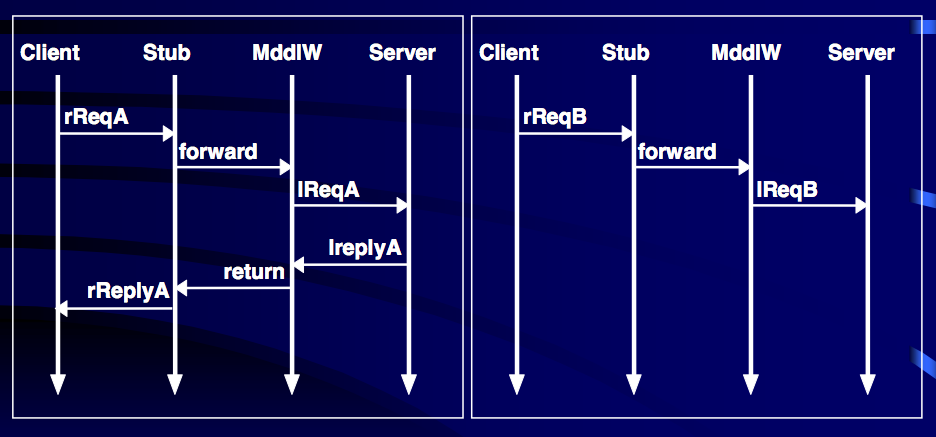
\includegraphics[scale=0.45]{Sintex.png}
\end{center}

Suponiendo que queremos que sólo esas trazas sean aceptables en nuestro sistema, surge el siguiente problema: cuando el \textit{middleware} recibe un \textit{forward}, ¿qué debe mandar? ¿\textit{IReqA} o \textit{IReqB}?. Dado que la respuesta depende de la interacción entre otro par de agentes, a menos que posea una visión global del sistema, el \textit{middleware} no tiene forma de saberlo.

Es evidente que la \textit{FSM} sintetizada puede tener trazas adicionales que no son deseadas en el sistema. O sea, vale que:
\begin{center}
	\fbox{Trazas del sistema $\subseteq$ Trazas de la FSM}
\end{center}

Pero:
\begin{center}
	\fbox{Trazas del sistema $\nsupseteq$ Trazas de la FSM}
\end{center}

\subsubsubsection{Escenarios implicados}
Formalmente, se define un \textbf{escenario} como un conjunto de trazas tal que, combinada con todos los otros escenarios, proveen una descripción completa del sistema. Uno en principio esperaría que dada uno un proceso correcto de síntesis, la \textit{FSM} tenga las mismas trazas (se comporten de igual manera). Sin embargo, dado que las componentes sólo poseen una visión local del sistema puede suceder que se comporten incorrectamente en términos de trazas del sistema. Es posible que algunos escenarios se combinen en formas no esperadas y que induzcan que ciertos comportamientos no presentes en la especificación del escenario aparezcan en todas las posibles implementaciones del sistema. A estos comportamientos se los llama \textbf{escenarios implicados}.

La existencia de escenarios implicados es un indicador de comportamiento no deseado en el sistema. Puede significar que:
\begin{itemize}
	\item Un escenario aceptable no fue tomado en cuenta (o sea, la especificación del escenario está incompleta).
	\item Un escenario inaceptable fue tomado en cuenta (o sea, la especificación del escenario es incorrecta). Esto denota una arquitectura incorrecta o muy abstracta.
\end{itemize}

Existen métodos de detección de escenarios implicados, que se basan en construir modelos locales, componerlos y detectar trazas que no están incluidas en un modelo global de la especificación.

~\newline
\underline{Ejemplo}:
\begin{center}
	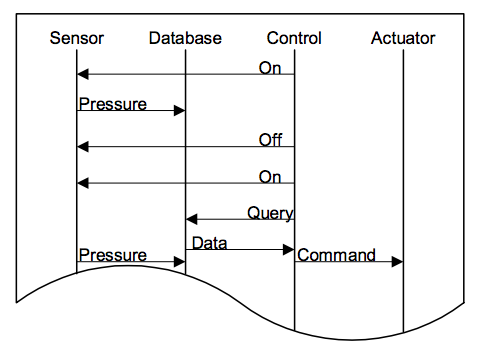
\includegraphics[scale=0.5]{Implicados.png}
\end{center}

La figura muestra una ejecución posible (aunque incorrecta) de la máquina. Sin embargo, cada componente se está comportando correctamente acorde con su especificación: El \textit{Sensor}, \textit{Control} y \textit{Actuator} están siguiendo los escenarios \textit{Initialise}, \textit{Register}, \textit{Terminate},  \textit{Initialise}, \textit{Analysis} y \textit{Register}. Sin embargo, \textit{Database} está siguiendo  \textit{Initialise}, \textit{Register}, \textit{Analysis} y \textit{Register}.

Esto se debe a que \textit{Control} no puede ver cuando \textit{Sensor} registró cosas en \textit{Database}, entonces si tiene que pedir información a \textit{Database} \textbf{después} de que haya sido submiteada por el \textit{Sensor}, debe esperar que \textit{Database} active y desactive los pedidos apropiadamente. Sin embargo, como \textit{Database} no puede saber cuando el sensor está o no activado, no puede hacerlo en los momentos correctos.

% The  Control component cannot see when the  Sensor has
% registered data in the Database, thus if it is to query the database
% after data has been registered at least once, it must rely on the
% Database to enable and disable queries when appropriate.
% However, as the Database cannot tell when the sensor has been
% turned on or off; it cannot distinguish a first registration of data
% from others. Thus, it cannot enable and disable queries
% appropriately. Succinctly, components do not have enough local
% information to prevent the system execution shown in Figure 7.
% Note that each component is behaving correctly according to
% some valid, but different, sequence of bMSCs. The  Sensor,
% Control and  Actuator are going through scenarios  Initialise,
% Register,  Terminate,  Initialise,  Analysis,  Register. However, the
% Database  is performing  Initialise,  Register,  Analysis,  Register.
% We will use the term implied scenario to refer to system
% executions such as the one shown in Figure 7.

\subsubsubsection{Extensiones}
A continuación se presentan algunas extensiones en diagramas de secuencia:
\subsubsubsubsection{Condiciones y estados}
\begin{center}
	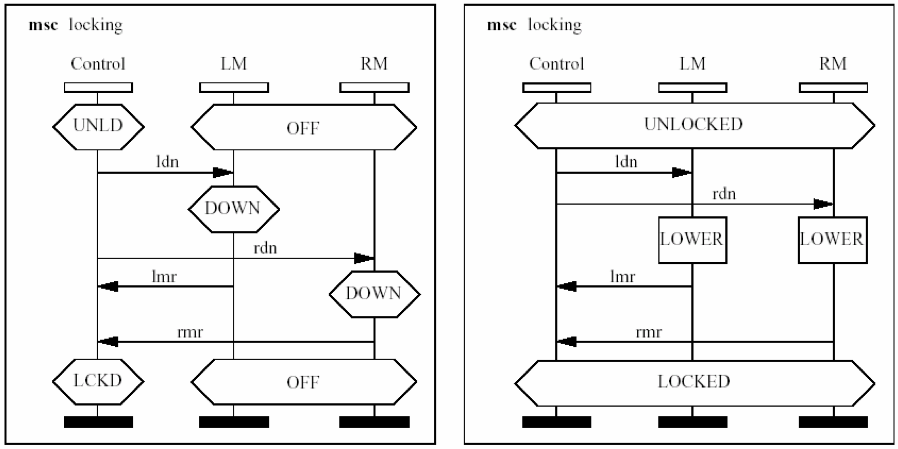
\includegraphics[scale=0.4]{CondEstados.png}
\end{center}

\subsubsubsubsection{Co-Regiones y Ordenamientos generales}
\begin{center}
	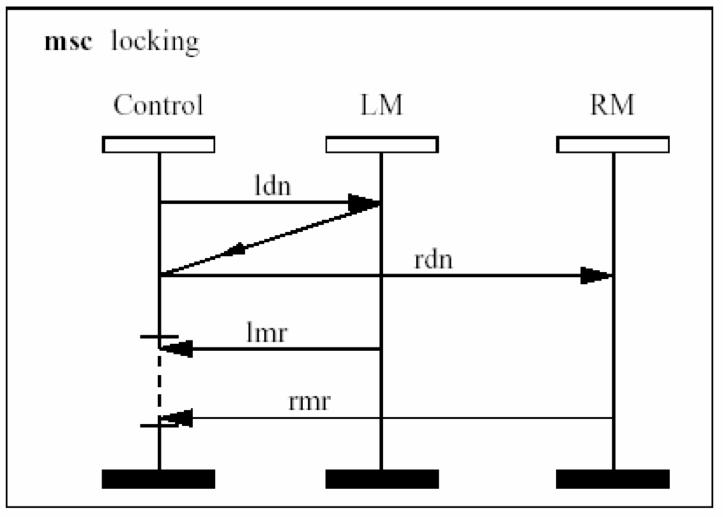
\includegraphics[scale=0.4]{CoRegOrd.png}
\end{center}

\subsubsubsubsection{Timers y TimeOuts}
\begin{center}
	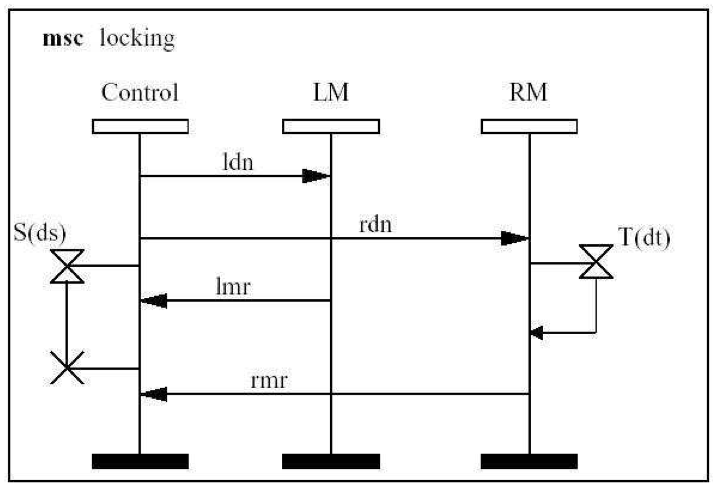
\includegraphics[scale=0.4]{TimTim.png}
\end{center}

\subsubsubsubsection{Mensajes Perdidos y Encontrados}
\begin{center}
	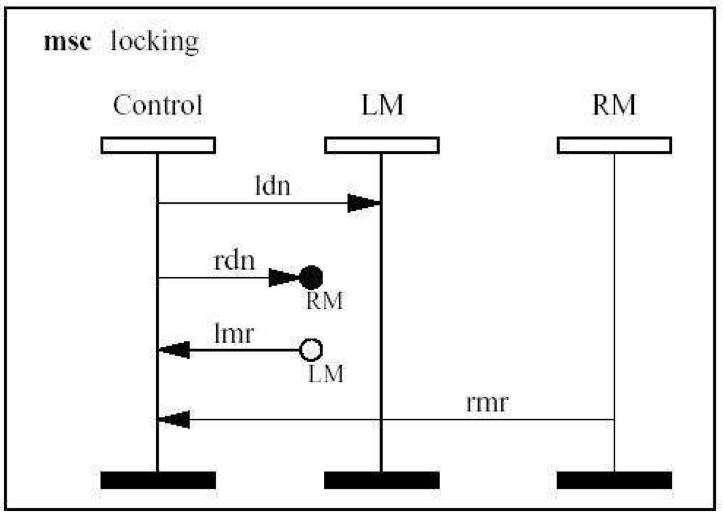
\includegraphics[scale=0.4]{MsgPerdEnc.png}
\end{center}

\subsubsubsubsection{Dynamic Creation and Destruction}
\begin{center}
	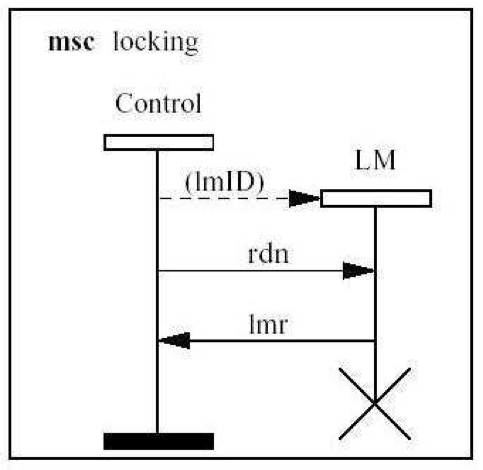
\includegraphics[scale=0.4]{DynCD.png}
\end{center}

\subsubsubsubsection{Gatillo o Trigger}
\begin{center}
	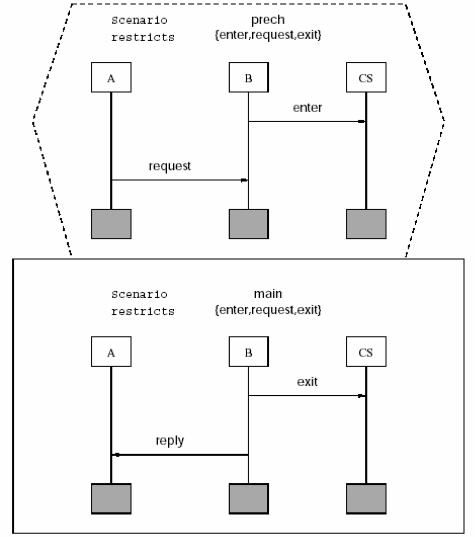
\includegraphics[scale=0.4]{Trigger.png}
\end{center}

\subsubsubsubsection{Alternativas, Ciclos y Paralelismo}
\begin{center}
	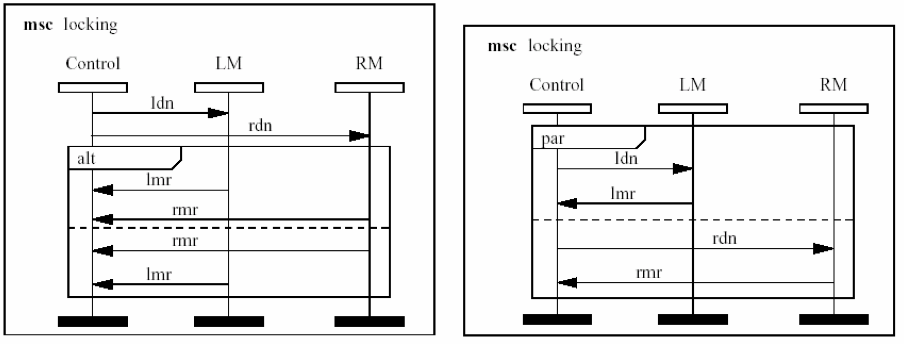
\includegraphics[scale=0.4]{AltCicPara.png}
\end{center}

\subsubsubsubsection{Barras de Activación y Returns}
\begin{center}
	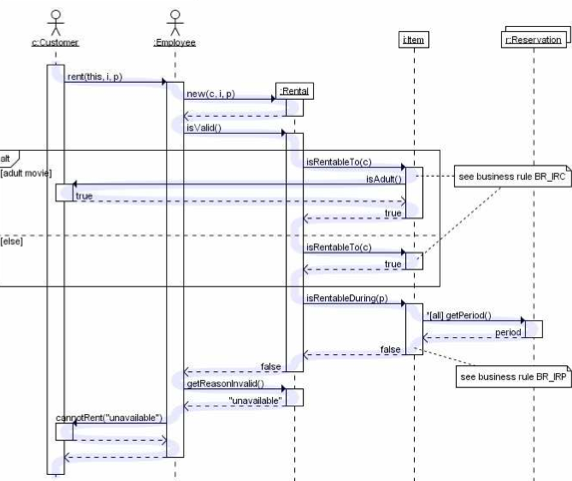
\includegraphics[scale=0.4]{Barract.png}
\end{center}

\subsubsection{Collaboration Diagrams}
Es una herramienta \textbf{basada en interacción} para expresar gráficamente comportamiento.
\begin{center}
	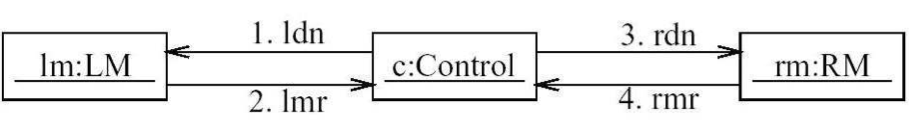
\includegraphics[scale=0.4]{Collab.png}
\end{center}

Sus características principales son:
\begin{itemize}
	\item Se enfoca en la estructura del sistema.
	\item Se numeran las interacciones, lo que permite establecer órdenes totales.
	\item No es apto pata trazas complejas.
\end{itemize}

\subsubsection{Redes de Petri}
Las redes de Petri son un modelo de comportamiento que poseen características de modelo basado en interacciones y basado en estados. Estructuralmente, son un digrafo bipartito con pesos asociados a lo ejes. Los dos conjuntos de la bipartición del grafo se denominan \textit{places} y \textit{transiciones}. Los \textit{places} que alimentan a una transición se denominan \textit{preset}, mientras que los que son alimentados por una transición se denominan \textit{poset}. Los nodos del tipo \textit{transiciones} están etiquetados.

Cada nodo de tipo \textit{place} puede contener 0 o más \textit{tokens}. Una asignación de \textit{tokens} a \textit{places} se denomina \textit{marking}. Existe un determinado \textit{marking inicial}. Una \textit{transición} $t$ puede dispararse sólo cuando la cantidad de \textit{tokens} en su \textit{preset} supera el peso de la arista que lo une con $t$. Una vez que se realiza esa \textit{transición} $t$, a cada uno de los \textit{posets} de esa transición se le suma una cantidad de \textit{tokens} igual al peso de la arista que une $t$ con el correspondiente \textit{poset}.

\begin{center}
	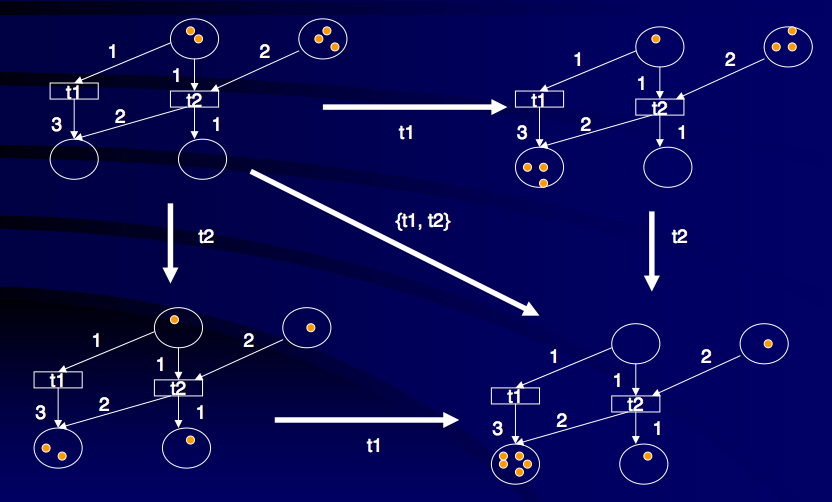
\includegraphics[scale=0.5]{Petri.png}
\end{center}

Se dice que un \textit{marking} es \textbf{alcanzable} si es el resultado de una secuencia de transiciones que resulten en ese \textit{marking}, partiendo desde el \textit{marking inicial}.

A su vez, se dice que una red de Petri es \textbf{\textit{n}-safe} no es alcanzable ningún \textit{marking} que contenga más de $n$ \textit{tokens} en un \textit{place}.

~\newline

Existen herramientas automáticas que permiten analizar propiedades e invariantes de las redes de Petri, tales como existencia de \textit{deadlocks}, alcanzabilidad, etc. Algunas de estas herramientas se basan en propiedades del álgebra lineal.

~\newline

\textbf{Características}
\begin{itemize}
	\item Formal, operacional, gráfico, refutable.
	\item Scope: concurrencia,control (uso similares a FSM).
	\item Semántica: sistema de transición u ordenes parciales.
	\item Mecanismo de descomposición: no standard.
	\item Al igual que las FSM, muchos tipos de análisis posibles.
	\item Relacióncon FSM: si es n-\textit{safe}, hay una relación de conversión en ambos sentidos.
	\item Muchas variantes: tiempo, probabilidades, datos, etc.
\end{itemize}
%PREGUNTAR TRUE CONCURRENCY

\subsubsection{Diagramas de Actividad}
Los diagramas de actividad son una versión \textit{user-friendly} de las redes de Petri. En ellos, cada estado tiene una semántica particular. El conjunto de todos los estados (con su respectiva semántica) presenta un \textbf{flujo de actividades}. Los estados están unidos por medio de flechas que representan un \textbf{flujo de control}.

Poseen ciertas características destacables:
\begin{itemize}
	\item Tienen soporte para asignación de responsabilidades, así como para concurrencia de actividades, entre otras.
	\item Son una visión global y temprana de \textit{proceso}.
	\item Proveen una descripción de paralelismo y coordinación.
	\item Aplicables a diseño y requerimientos.
\end{itemize}

Permite vincular casos de uso:
\begin{itemize}
	\item Mostrando la secuencia de un caso de uso.
	\item Reflejando las interacciones entre varios casos.
	\item Modelando el comportamiento interno del sistema.
\end{itemize}

\subsubsubsection{Decisión}
Un diagrama de actividad expresa una decisión cuando una condición es usada para indicar diferentes transiciones posibles que dependen de un valor booleano. El ícono provisto para una decisión es un diamante, con una o más flechas entrantes y con dos o más flechas salientes, cada una etiquetada por una condición diferente y sin evento que la dispare.

Todos los posibles valores para la condición deben aparecer en las transiciones salientes: debe ser completo y determinístico. Si no se especifican las condiciones en las flechas salientes, puede interpretarse como una elección aleatoria equiprobable en la cantidad de flechas salientes.

\begin{center}
	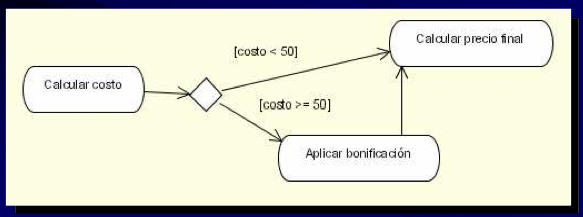
\includegraphics[scale=0.5]{ActivDeci.png}
\end{center}

\subsubsubsection{Fork y Join}
Permiten establecer concurrencia entre acciones. El operador de \textit{Fork} separa la ejecución en dos o más ramas. Obligatoriamente todas las ramas se siguen y no es posible hacer ningún tipo de asunción sobre el orden en el que se van a realizar, puesto que no está especificado.

Después de un operador \textit{fork}, el hijo de ejecución se vuelve a unir con uno o más operadores \textit{join}. Estos operadores toman dos hilos de ejecución distintos y lo convierten en uno sólo. Para que se continúe la ejecución en un \textit{join} es necesario que \textbf{todos} los hilos de ejecución que desembocan en ese \textit{join} hayan llegado a él.

\begin{center}
	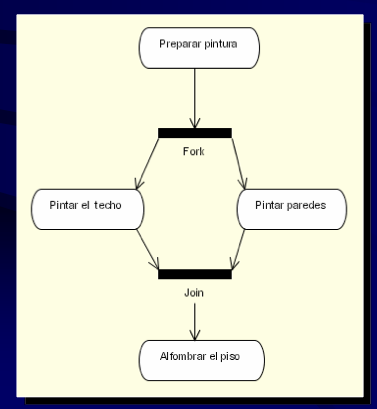
\includegraphics[scale=0.5]{ForkJoin.png}
\end{center}

\subsubsubsection{Andariveles}
Los andariveles permiten la asignación de responsabilidad en los diagramas de actividad. Las acciones se organizan en andariveles, que corresponden uno a cada ``unidad organizacional'' (en general existe una relación entre estos y los actores de los casos de uso). Si una actividad cae dentro del andarivel de un actor $t$, entonces es ese actor $t$ quien tiene la responsabilidad por la susodicha acción.

%%NUEVO-COBY%%
También puede verse una analogía entre cada estado del diagrama de actividad con un caso de uso del modelo de operaciones.
%%FIN-NUEVO-COBY%%


\begin{center}
	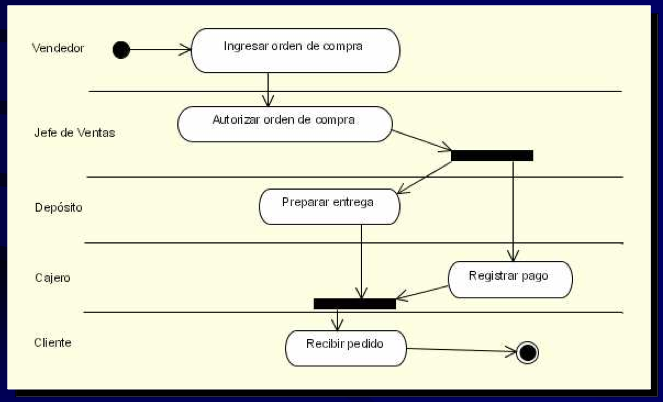
\includegraphics[scale=0.5]{Andariveles.png}
\end{center}

\subsubsection{Diseño vs Requerimientos}
Los modelos de comportamiento pueden usarse para describir el diseño:
\begin{itemize}
	\item Los eventos pueden ser llamadas a métodos, procedimientos, mensajes, interrupciones, etc.
	\item Las entidades pueden ser procesos, módulos, objetos, threads, etc.
\end{itemize}

~\newline
A su vez, también pueden ser usados para describir el dominio.

\newpage

\section{Máquinas de estado}
Según las diapositivas, es un área con un ``despelote terminológico''. Una \textbf{máquina de estado} es un término genérico que denota una familia de notaciones que tienen \textbf{estados} (discretización del estado), \textbf{transiciones} (relación ``sigue a'') y \textbf{etiquetas} (enriquecen la noción de estado y transición).

~\newline
\underline{Ejemplos}:

\begin{itemize}
	\item Statechart.
	\item \textit{FSM} (Finite State Machines).
	\item \textit{LTS} (Labelled Transition System).
	\item Automata.
	\item Timed Automata.
\end{itemize}

%Se denomina máquina de estados a un modelo de comportamiento de un sistema con entradas y salidas, en donde las salidas dependen no sólo de las señales de entradas actuales sino también de las anteriores. Las máquinas de estados se definen como un conjunto de estados que sirve de intermediario en esta relación de entradas y salidas, haciendo que el historial de señales de entrada determine, para cada instante, un estado para la máquina, de forma tal que la salida depende únicamente del estado y las entradas actuales.
~\newline
Las máquinas de estados estructuran el mundo de acuerdo con la relación \textit{``sigue a''}, permitiendo representar secuencias de estado de manera compacta. Esto genera que tengan numerosos usos, tales como:
\begin{itemize}
	\item Descripción del problema y la solución.
	\item En ingeniería de requerimientos, se usan para graficar el comportamiento de agentes y estados de entidades pasivas.
	\item En diseño, se usan para protocolos, arquitecturas de software, estados de objetos y clases, etc.
\end{itemize}

%%NUEVO-COBY%%
\underline{Diferencias entre Diagrama de Actividad y FSM:} la manera de cómo describir el comportamiento. En DA se ve fácil porque la semántica importante está en los estados. En FSM, en cambio, el foco está en las transiciones. Por esta razón puedo escribir para una máquina otra que tenga las mismas trazas pero con diferente cantidad de estados. Además, en DA se podía interpretar paralelismo o simultaneidad con un Fork; en realidad, daba una idea de independencia de acciones y no conocemos su orden. En FSM se podrá decir esto explpicitamente con composición en paralelo: se ejecutan etiquetas compartidas si hay sincronización, todas las máquinas con esa etiqueta deben estar listas, por eso hay simultaneidad.
%%FIN-NUEVO-COBY%%

\subsection{LTS: Labelled Transition Systems}
Informalmente, un \textit{LTS} es un tipo de máquina de estados. Se caracteriza por tener transiciones etiquetadas (eventos instantáneos) y que los estados sean semánticamente nulos, excepto uno que indica el estado inicial de la máquina (pueden etiquetarse por comodidad de lectura o referencia, pero no es relevante a los efectos de la semántica). Se utiliza para \textbf{describir comportamiento de entidades} y \textbf{razonar sobre el comportamiento emergente resultante de su ejecución concurrente}.

Formalmente, se define una LTS de la siguiente manera:

\caja{0.8}{
Sea \textit{Estados} el universo de estados posibles y \textit{Act} el universo de acciones observables. Además, definimos \textit{Act}$_{\tau,\in}$ = \textit{Act} $\bigcup$ $\{\tau\}$ $\bigcup$ $\{\in\}$, siendo $\tau$ la acción \textit{no observable} o \textit{silenciosa} y $\in$ la acción \textit{nula}.

~\newline

 Un \textit{\textbf{LTS}} es una tupla $P = <S,L,\Delta,s_o>$, donde
\begin{itemize}
	\item $S \subseteq $ \textit{Estados} es un conjunto de estados finito.
	\item $L \subseteq$ \textit{Act}$_{\tau,\in}$ es un conjunto de etiquetas.
	\item $\Delta \subseteq (SxLxS)$ es un conjunto de transiciones etiquetadas.
	\item $s_0 \in S$ es el estado inicial.
\end{itemize}
Definimos el \textbf{alfabeto de comunicación} de $P$ como $\alpha(P) = L \backslash \{\tau,\in\}$
}

\underline{Observación}: $L$ también es llamado $\sum$ o $\sum^*$ si incluye la transición $\in$.

~\newline


\underline{Ejemplo}:
\begin{center}
	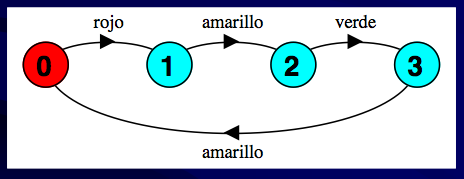
\includegraphics[scale=0.5]{LTSe.png}
\end{center}

~\newline

\underline{Observación}: El conjunto de etiquetas de un \textit{LTS} no tiene por qué ser minimal. Pueden existir etiquetas que no se usen y sin embargo sí siguen categorizando como etiquetas compartidas y, como tales, vale la regla de paralelización de etiquetas compartidas.

\subsubsection{Semántica}
\subsubsubsection{Ejecución}
Sea $P = (S,L,\Delta,q)$ una \textit{LTS}. Se define una \textbf{ejecución} de $P$ como una secuencia $w = q_0,l_0,q_1,l_1, \hdots$ de estados $q_i \in S$ y transiciones $l_i \in L$ tal que
\begin{itemize}
	\item $q_0 = q$
	\item $\displaystyle \forall \ 0 \leq i \leq \left | \frac{w}{2}\right |$ : $(q_i,l_i,q_{i+1}) \in \Delta$
\end{itemize}

\subsubsubsection{Proyección}
Sean $w$ una palabra $w_0,w_1,w_2,\hdots$ y $A$ un alfabeto. Se define la \textbf{proyección} de $w$ sobre $A$ (que se nota $w|_A$) como el resultado de eliminar de $w$ todos los elementos $w_i$ tales que $w_i\not\in A$.

\subsubsubsection{Trazas}
Informalmente, una traza de un \textit{LTS} es, dada una ejecución, quitarle los estados (o sea, quitar las etiquetas). No me importa por qué estado pasé. Lo único que me importa son los estímulos y reacciones de un agente, no el agente mismo.

Formalmente, sea $P = (S,L,\Delta,q)$ una \textit{LTS}. Una palabra $w$ del alfabeto $\alpha(P)$ es una \textbf{traza} de $P$ si existe una ejecución $w'$ tal que $\displaystyle w=w'|_{\alpha(P)}$.

A su vez, definimos $tr(P)$ como el conjunto de todas las trazas de la \textit{LTS} $P$.
\begin{center}
	\fbox{$tr(P) = \{w | w $ es traza de $P\}$}
\end{center}

Otra definición alternativa es que
\begin{center}
	\fbox{$Tr(s) = \{\alpha | \alpha\in\sum^* \text{ y } s\flecha{a}s'\}$}\\
	\fbox{$Tr(L) = Tr(s_0)$}
\end{center}

Decimos que un \textit{LTS} satisface una propiedad si y sólo si \textbf{todas} sus trazas la satisfacen. Sin embargo existen propiedades que no se pueden examinar sobre las trazas sino sobre el \textbf{branching} (semántica arbórea). Un ejemplo de esto son los casos de uso.

Se define el conjunto de estados \textbf{alcanzables por $\alpha$} de la siguiente manera:
\begin{center}
	\fbox{$Alc(s,\alpha) = \{s' | s\flecha{\alpha}s'\}$}
\end{center}

Se define que un \textit{LTS} $L$ tiene \textbf{comportamiento finito} si existe un $n\in \mathbb{N}$ tal que para toda traza $\sigma \in Tr(L)$, la longitud de $\sigma$ es menor que $n$.

%%NUEVO-COBY%%
Una traza informalmente se puede describir como una tira de etiquetas o cadena de transiciones.
%%FIN-NUEVO-COBY%%

\subsubsubsection{Transición o Evolución}
Sea $P = (S,L,\Delta,q)$ una \textit{LTS}. Decimos que $P$ \textbf{transita} o \textbf{evoluciona} con una etiqueta $l$ en un nuevo \textit{LTS} $P'$ si $P'=(S,L,\Delta,q')$ y $(q,l,q')\in\Delta$. Se nota $P \flecha{l} P'$.


\subsubsection{Concurrencia vs Paralelismo}
\begin{savenotes}
\begin{center}
	\begin{tabular}{|p{6cm}|p{6cm}|}
		\hline
		\textbf{Concurrencia} &  \textbf{Paralelismo}\\ \hline \hline
		Procesamiento lógicamente simultáneo & Procesamiento físicamente simultáneo\\ \hline
		No necesariamente implica múltiples unida	des de procesamiento\footnote{Si hay una sola unidad de procesamiento, es necesario utilizar ejecución \textit{interleaved}.} & Involucra múltiples unidades de procesamiento\\ \hline
	\end{tabular}
\end{center}
\end{savenotes}

Tanto concurrencia como paralelismo requieren acceso controlado a recursos comunes.

\subsubsection{Composición en paralelo}
Informalmente, la \textbf{composición en paralelo} de dos \textit{LTS} construye una nueva \textit{LTS} que permite casi todas las combinaciones posibles de las acciones de los dos alfabetos. Las acciones que pertenezcan a ambos alfabetos deben ser ejecutadas por ambos procesos simultáneamente. Estas acciones compartidas \textbf{sincronizan} la ejecución de los dos procesos. Es por esto que se dice que las \textbf{interacciones} o \textbf{acciones compartidas} \textit{restringen el comportamiento global}.

Semánticamente, si suponemos que cada \textit{LTS} modela un agente o proceso y ese agente quiere hacer alguna acción que nadie más monitorea, entonces la puede hacer sólo, en cualquier momento y todo el resto queda igual. Si, en cambio, esa acción está en la interfaz de otro agente/proceso, entonces tienen que hacerla en conjunto.
~\newline

Formalmente, la \textbf{composición en paralelo} es una función $|| : LTS^n \rightarrow LTS$.

Sean $P_1 = (S_1,L_1,\Delta_1,q_1)$ y $P_2 = (S_2,L_2,\Delta_2,q_2)$ dos \textit{LTS}. La \textbf{composición en paralelo} de $P_1$ y $P_2$ (notada $P_1 || P_2$), es un nuevo \textit{LTS} $(S_1xS_2,L_1xL_2,\Delta,(q_1,q_2))$, donde $\Delta$ es la relación más pequeña que satisface:
\begin{multicols}{2}
\begin{itemize}
	\item $\displaystyle \frac{P_1 \flecha{l} P_1'}{P_1||P_2 \flecha{l} P_1'||P_2}$  $\hspace*{1cm}(l\not\in\alpha(P_2))$
	\item $\displaystyle \frac{P_2 \flecha{l} P_2'}{P_1||P_2 \flecha{l} P_1||P_2'}$  $\hspace*{1cm}(l\not\in\alpha(P_1))$
	\item $\displaystyle \frac{P_1 \flecha{l} P_1' \hspace*{0.5cm} P_2 \flecha{l} P_2'}{P_1||P_2 \flecha{l} P_1'||P_2'}$  $\hspace*{1cm}(l\neq\tau)$
\end{itemize}
\end{multicols}

\underline{Ejemplo}:

\begin{center}
	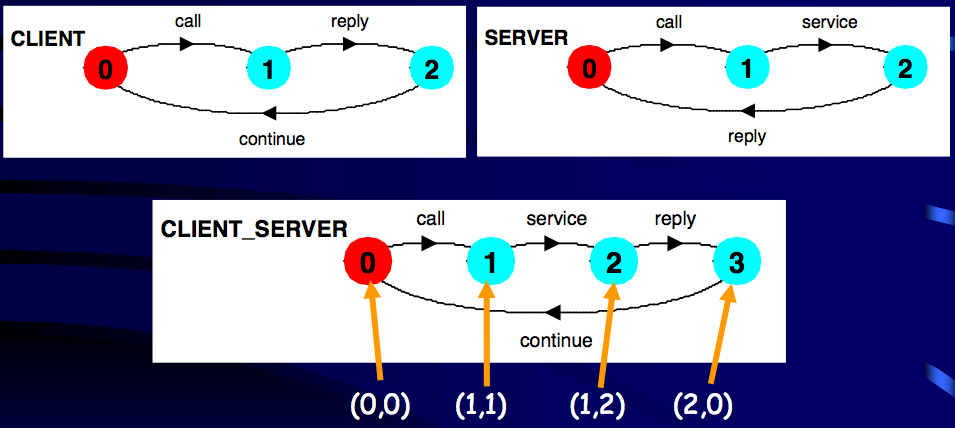
\includegraphics[scale=0.4]{ComParal.png}
\end{center}

~\newline

\paragraph{Leyes Algebráicas de composición}
\begin{itemize}
	\item Conmutatividad: $(P||Q) = (Q||P)$
	\item Asociatividad: $(P||(Q||R)) = ((P||Q)||R) = (P||Q||R)$
\end{itemize}

Observar que la propiedad de reflexividad ($P||P = P$) \textbf{no} vale en el caso general, como se puede ver en el siguiente contraejemplo:
\begin{center}
	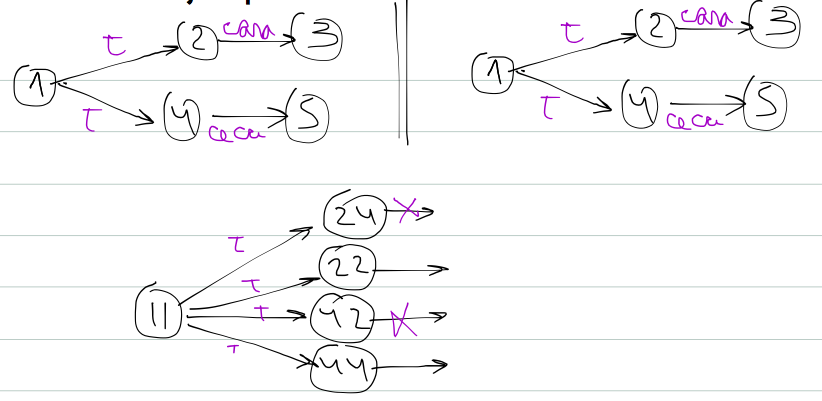
\includegraphics[scale=0.5]{Contraejemplo.png}
\end{center}

Sin embargo, \textbf{sí} vale para \textit{LTS} determinísticos.

\subsubsection{Modelado de Concurrencia}
Para el análisis con \textit{LTS} asumimos que las máquinas pueden funcionar a velocidades arbitrarias, abstrayendo el tiempo. Para modelar concurrencia se supone un orden arbitrario de acciones de los distintos procesos (se hace \textbf{interleaving} de acciones pero se preservan las acciones de cada proceso). Esto trae como resultado un modelo general, independiente de la política de scheduling (modelo de ejecución \textbf{asincrónico}).

O sea no se asume nada sobre la velocidad individual de los procesos ni del scheduler que los gobierna.

\subsubsection{LTS no determinístico}
Un \textit{LTS} se dice \textbf{no-determinístico} si tiene al menos un estado con más de una transición etiquetada con la misma acción. Esto permite abstraer los detalles involucrados en la toma de una decisión.

Formalmente, un \textit{LTS} es \textbf{determinístico} si $\forall \sigma \in \sum^*$, $\#Alc(s_0,\sigma)\leq 1$.

Toda máquina de estados no determinística puede convertirse en una determinística con las mismas trazas. Pero puede tomar una cantidad exponencial de estados.
~\newline

\underline{Ejemplo}:
\begin{figure}[htb]
 \begin{center}
   \leavevmode
   \includegraphics[scale=0.40]{Deter.jpg}
   \includegraphics[scale=0.40]{NoDeter.png}
 \end{center}
\end{figure}


\subsubsection{Propuestas para la igualdad de LTS}

¿Cómo se establece la comparación entre dos \textit{LTS}? Hay varias propuestas:

\subsubsubsection{Propuesta 1: Isomorfismo}
``Dos \textit{LTS} son equivalentes si sus grafos subyacentes son isomorfos''. Esta propuesta falla como se puede ver en el siguiente contraejemplo:
\begin{figure}[htb]
 \begin{center}
   \leavevmode
   \includegraphics[scale=0.5]{Isom1.png}
   \includegraphics[scale=0.5]{Isom2.png}
 \end{center}
\end{figure}

Claramente querríamos que estos dos \textit{LTS} fueran equivalentes (porque los estados tienen semántica nula), pero sus grafos subyacentes no son isomorfos.

\subsubsubsection{Propuesta 2: Isomorfismo sin estados alcanzables}
``Dos \textit{LTS} son equivalentes si al quitar sus estados no alcanzables son isomorfos''. Esta propuesta falla como se puede ver en el siguiente contraejemplo:
\begin{center}
	\includegraphics[scale=0.5]{Isomor.png}
\end{center}

En este caso, querríamos estos dos \textit{LTS} fueran equivalentes, pero sus grafos subyacentes, aún retirando estados no alcanzables, no son isomorfos.


\subsubsubsection{Propuesta 3: Igualdad de Trazas}\label{trazfail}
``Dos \textit{LTS} son equivalentes si definen el mismo conjunto de trazas''. Esta propuesta falla como se puede ver en el siguiente contraejemplo:
\begin{center}
	\includegraphics[scale=0.5]{TrazFail.png}
\end{center}

%%NUEVO-COBY%%
En este ejemplo no deberíamos querere ver ambas máquinas como iguales porque la de la izquierda es no-determinista y la derecha es determinista.
%%FIN-NUEVO-COBY%%


Claramente, la equivalencia por trazas es una equivalencia demasiado gruesa (\textit{coarse}) o débil (\textit{weak}). Puede ser que una composición de dos \textit{LTS} ``iguales'' por trazas con la misma \textit{LTS} las vuelva distinguibles.

%%NUEVO-COBY%%
Igualmente, la igualdad de trazas en \textbf{LTS determinísticas} sí es lo mismo que la bisimulación fuerte.
%%FIN-NUEVO-COBY%%


\subsubsubsection{¿Qué buscamos?}
Para la equivalencia de \textit{LTS} estamos buscando una relación que verifique:
\begin{itemize}
	\item Ser de equivalencia:
	\begin{itemize}
		\item Reflexiva: $P \equiv P$
		\item Transitiva: $(P \equiv Q \wedge Q \equiv R) \Rightarrow (P \equiv R)$
		\item Simétrica: $(P \equiv Q) \Rightarrow (Q \equiv P)$
	\end{itemize}
	\item Ser abstracta con respecto a:
	\begin{itemize}
		\item Número de estados del modelo.
		\item Estructura del modelo.
		\item Trazas del modelo.
	\end{itemize}
	\item Coincida con nociones empíricas.
	\item Mantenga coherencia con nuestro lenguaje de especificación (por ejemplo, $(P \equiv Q) \Rightarrow P||R \equiv Q||R$).
\end{itemize}

\subsubsection{Bisimulación}
Sea $P$ el universo de todos los \textit{LTS}. Una relación binaria $R\subseteq PxP$ es una \textbf{bisimulación fuerte} si y sólo si cuando $(P,Q)\in R$ entonces para cada $a\in Act$:
\begin{itemize}
	\item $(P\flecha{a}P')\Rightarrow (\exists Q' : Q\flecha{a}Q' \wedge (P',Q')\in R)$
	\item $(Q\flecha{a}Q')\Rightarrow (\exists P' : P\flecha{a}P' \wedge (P',Q')\in R)$
\end{itemize}

Sean $P$ y $Q$ dos $LTS$. Se define que $P$ y $Q$ son \textbf{fuertemente bisimilares} (y se nota $P \sim Q$) si y sólo si existe una bisimulación fuerte $R$ tal que $(P,Q)\in R$.
\begin{center}
	$\sim =\bigcup\{R|R$\textit{ es una bisimulación fuerte}$\}$
\end{center}

~\newline

De estas dos definiciones se puede extraer una versión ``compacta'':

\caja{0.5}{
	\textit{$P\sim Q$ si para cada acción $a\in$ Act}
	\begin{itemize}
		\item $(P\flecha{a}P')\Rightarrow(\exists Q' : Q\flecha{a}Q' \wedge P'\sim Q')$
		\item $(Q\flecha{a}Q')\Rightarrow(\exists P' : P\flecha{a}P' \wedge P'\sim Q')$
	\end{itemize}
}

%%NUEVO-COBY%%
Informalmente, $M_2$ simula una máquina $M_1$ si para toda etiqueta $a$ vale que: $M_1$ puede hacer $a$ $\Rightarrow$ $M_2$ puede hacer $a$. Las máquinas $M_1$ y $M_2$ son bisimilares cuando $M_1$ simula a $M_2$ y viceversa.
%%FIN-NUEVO-COBY%%


\subsubsubsection{No-bisimilaridad}
Para demostrar la bisimilaridad entre dos \textit{LTS} $P$ y $Q$ alcanza con dar la relación de bisimulación que se utiliza. Sin embargo, para demostrar la no-bisimilaridad se debe enumerar todas las relaciones binarias y mostrar que ninguna contiene a $(p_0,q_0)$ (siendo $p_0$ el estado inicial de $P$ y $q_0$ el de $Q$) y es una bisimulación fuerte. El problema de esto es que es notablemente costoso. Es por esto, que es más frecuente utilizar un \textbf{juego} que permite determinar sencillamente la bisimilaridad (o falta de) entre dos \textit{LTS}.

El juego consiste en un \textbf{atacante}, que intenta probar que $P \not \sim Q$ y un \textbf{defensor}, que intenta probar que $P\sim Q$. Cada \textbf{ronda} del juego tiene una \textbf{configuración}, un par ordenado $(S,T)$. El juego comienza con la configuración $(P,Q)$.

%El juego consiste en un \textbf{atacante}, que intenta probar que $P \not \sim Q$ y un \textbf{defensor}, que intenta probar que $P\sim Q$. Cada \textbf{ronda} del juego tiene una \textbf{configuración}, que es un par de $(????) x (????)$. El juego comienza con la configuración $(P,Q)$.


En cada ronda, el atacante elige uno de los procesos de la configuración actual y hace una movida por alguna transición con etiqueta $a \in A$. El defensor debe responder haciendo una movida etiquetada por $a$ en el otro proceso. Si un jugador no puede mover, el otro gana. Si el juego sigue infinitamente, gana el defensor (o sea, $P\sim Q$).

\begin{itemize}
	\item $P$ y $Q$ son fuertemente bisimilares si y solo si el defensor tiene una estrategia ganadora universal empezando desde la configuración $(P, Q)$.
	\item $P$ y $Q$ no son fuertemente bisimilares si y solo si el atacante tiene una estrategia ganadora universal empezando desde la configuración $(P, Q)$
\end{itemize}

\subsubsection{Congruencia}
Dado un contexto para $P$, querríamos poder cambiar $P$ por un proceso $Q$ equivalente sin alterar el sistema. Se define entonces una \textbf{equivalencia} entre $P$ y $Q$ como una congruencia en $P \equiv Q \Rightarrow C(P)\equiv C(Q)$. Dos procesos son equivalentes si un observador externo no los puede distinguir.

\begin{center}
	\includegraphics[scale=0.5]{Equiv.png}
\end{center}


\subsubsection{Semántica lineal vs semántica arbórea}
Plantear la equivalencia de trazas induce una semántica lineal: un \textit{LTS} queda caracterizado por un conjunto de secuencias.

\begin{center}
	\includegraphics[scale=0.5]{SemLineal.png}
\end{center}

Para algunas aplicaciones, la semántica lineal es más apropiado (por ejemplo, en situaciones donde lo más intuitivo es dar propiedades de las trazas).

~\newline

A diferencia de esto, plantear una equivalencia por bisimulacíón induce una semántica arbórea: un \textit{LTS} queda caracterizado por el árbol de ejecución resultante de desdoblar sus ciclos.

\begin{center}
	\includegraphics[scale=0.5]{SemArbol.png}
\end{center}

Para otras aplicaciones, es necesario utilizar semántica arbórea (por ejemplo, para \textit{composición en paralelo}, \textit{casos de uso} o cualquier propiedad de tipo \textit{branching}).

Existen ciertas lógicas temporales lineales y branching que permiten predicar sobre conjuntos de trazas y estructuras arbóreas.

%%NUEVO-COBY%%
O sea, equivalencia por trazas pide igualdad de trazas; mientras que equivalencia por bisimulación pide isomorfismo de árboles de ejecución.
%%FIN-NUEVO-COBY%%


\subsubsection{Tau $\tau$}
Cómo se vio en su definición, los \textit{LTS} vienen equipados con una etiqueta especial, $\tau$, que representa una acción interna, no observable\footnote{Una acción es \textbf{observable}, si puede ser usada para comprobar la respuesta del sistema frente a un estímulo.} y no controlable\footnote{Una acción es \textbf{controlable}, si puede ser usada para estimular al sistema.} desde el mundo exterior. Es muy utilizada para:
\begin{itemize}
	\item Impedir sincronización externa (por ejemplo, si dos máquinas tienen \textit{timeout}, tenderían a sincronizarse. Con $\tau$ eso no pasa).
	\item Abstraer acciones interna, reduciendo la complejidad.
\end{itemize}

\subsubsection{Bisimulación considerando $\tau$}
Considerando la etiqueta $\tau$ y su comportamiento, es necesario reconsiderar la noción de bisimulación. Es necesario que la relación de bisimulación ``elimine'' las transiciones etiquetadas por $\tau$, porque al ser acciones internas, no deberían tener inferencia en la relación.

\begin{center}
	\includegraphics[scale=0.5]{BisimTau.png}
\end{center}

Es por esto que definimos las \textbf{transiciones observacionales débiles}:

\begin{equation}
  \displaystyle \overset{\displaystyle a}{\displaystyle \Rightarrow}=\begin{cases}
   \displaystyle  (\flecha{\displaystyle \tau})^*\circ \flecha{\displaystyle a} \circ (\flecha{\displaystyle \tau})^*, & \text{si $\displaystyle a\neq\tau$}.\\
 \displaystyle    (\flecha{\displaystyle \tau})^*, & \text{si $\displaystyle a=\tau$}.
  \end{cases}
\end{equation}

% \begin{center}
% 	\includegraphics[scale=0.5]{TransDebil.png}
% \end{center}

Esto nos permite definir un concepto de \textbf{bisimilaridad débil}. Intuitivamente, ``si $P$ hace la acción $a$, entonces $Q$ lo debe imitar haciendo una acción $a$ y una cantidad arbitraria de $\tau$''.

Formalmente, sea $P$ el universo de todos los $LTS$. Una relación binaria $R\subseteq PxP$ es una \textbf{bisimulación débil} si y sólo si cuando $(P,Q)\in R$, entonces para cada acción $a\in Act\bigcup \{\tau\}$:
\begin{itemize}
	\item $(P\flecha{a}P')\Rightarrow(\exists Q' : Q \Flecha{a}Q' \wedge (P',Q')\in R)$
	\item $(Q\flecha{a}Q')\Rightarrow(\exists P' : P \Flecha{a}P' \wedge (P',Q')\in R)$
\end{itemize}

Análogamente, sean $P$ y $Q$ dos $LTS$. Se define que $P$ y $Q$ son \textbf{débilmente bisimilares} (y se nota $P \approx Q$) si y sólo si existe una bisimulación débil $R$ tal que $(P,Q)\in R$.
\begin{center}
	$\approx =\bigcup\{R|R$\textit{ es una bisimulación débil}$\}$
\end{center}

\subsubsubsection{Propiedades de bisimulación débil}
$\approx$...
\begin{itemize}
	\item ...es una relación de equivalencia.
	\item ...tiene un juego que la caracteriza (es igual que el anterior, pero el defensor puede hacer $\Rightarrow$).
	\item ...\textbf{bisimilaridad fuerte implica bisimilaridad débil} ($\sim \subseteq \approx$).
	\item ...es una congruencia con respecto al operador de composición en paralelo.
	\item ...abstrae los loops sobre $\tau$.
\end{itemize}

\begin{center}
	\includegraphics[scale=0.5]{LoopTau.png}
\end{center}

\subsubsubsection{Modelado con \textit{LTS}}
Un \textit{LTS} puede modelar un \textbf{agente}. Los eventos son fenómenos monitoreables o controlables, mientras que las trazas o árboles de ejecución describen la relación temporal esperada entre lo monitoreable y lo controlable (la sincronización de \textit{LTS} representa la relación \textit{monitoreabilidad-controlabilidad}).

Un \textit{LTS} puede modelar una \textbf{entidad pasiva}. Eventos son fenómenos aplicados a la entidad (i.e. operaciones sobre o que afectan la entidad). Explica el protocolo de uso esperado de la entidad.


\subsection{Autómatas temporizados}
Los \textit{LTS} tienen serios problemas de expresividad a la hora de trabajar con los tiempos que transcurren entre o durante las acciones. Es por esto que se aumenta la definición de \textit{LTS} de la siguiente manera:
\begin{itemize}
	\item Un \textbf{estado} del sistema es un par $(s,v)$ con:
	\begin{itemize}
		\item $s\in S$
		\item $v\in V$
		\item $Is[v] = true$
	\end{itemize}
	\item La arista $a = <s,l,\Psi,\alpha,s'>$ puede ser atravesada desde el estado $(s,v)$ sólo si $v$ satisface la condición $\Psi$.
	\item El estado resultante $(s',v')$ es tal que $\alpha(v) = v'$.
	\item El tiempo pasa sólo en los nodos.
	\item Atravesar una arista no insume tiempo.
	\item Los valores de los relojes crecen \textbf{uniformemente} con el tiempo.
	\item El sistema puede permanecer en un nodo $s$ mientras los valores de los relojes satisfagan $Is$.
\end{itemize}

\subsubsection{Semántica}
Proveer de semántica a los autómatas temporizados se lo hace en términos otra notación conocida: el \textit{LTS}. Es por esto que se dice que la semántica de \textit{TA} (Timed-Automata) \textbf{hereda} una relación de bisimulación y una relación de composición en paralelo.

\begin{center}
	\includegraphics[scale=0.6]{AuTemp.png}
\end{center}

~\newline

Formalmente, es un sistema de transición de estados etiquetados $T=<Q,\rightarrow>$, en donde $Q$ representa los estados ($Q=\{(s,v)\in S : Is[v]=true\}$) y $\rightarrow$ representa la relación de transición ($\rightarrow \subseteq Q x \{L \bigcup \mathbb{R}+\} \times Q$)\footnote{Esto se debe a que es un conjunto infinito.}.

Estas transiciones se dividen en dos subtipos:
\begin{itemize}
	\item \textbf{Temporales}: el paso de un tiempo $t$ es representado por una transición etiquetada por $t$.
	\begin{center}
		$\displaystyle \frac{Is[v+t], 0\leq t}{(s,v)\rightarrow t (s,v+t)}$
	\end{center}
	\item \textbf{Instantáneas}: dadas por la ejecución de una acción $e$. La transición lleva la etiqueta $e$.
	\begin{center}
		$\displaystyle \frac{<s,e,\Psi,\alpha,s'>\in A, \Psi[v] \text{ y } \alpha(v)=v'}{(s,v)\rightarrow e (s',v')}$
	\end{center}
\end{itemize}

Por comodidad de notación, se escribe $q \overset{e}{\rightarrow} q'$ en vez de $(q,e,q')\in\rightarrow$.

\subsection{Statecharts}
Un \textit{statechart} es un tipo de máquina de estado utilizado para diagramar comportamiento de un sistema. Su principal característica es que presentan estados \textbf{jerárquicos} y \textbf{ortogonales}.

\begin{center}
	\includegraphics[scale=0.5]{Statechart.png}
\end{center}

Otros aspectos que los caracterizan son:
\begin{itemize}
	\item Se distinguen los eventos \textbf{internos} de los \textbf{externos}.
	\item Sólo puede haber un evento externo por vez.
	\item Hay \textit{broadcasting} de eventos.
	\item Las transiciones se etiquetan con un par \textit{causa / efecto}.
	\item Colas de eventos.
	\item Transiciones multi-nivel.
\end{itemize}

\subsection{SDL Flowchart}
\begin{center}
	\includegraphics[scale=0.6]{SDLFlowchart.png}
\end{center}

\subsection{Relación con otros modelos}
\begin{itemize}
	\item \textbf{Diagrama de contexto}: Define cuál es la relación temporal entre los fenómenos en la interfaz de un agente. Existen variantes de \textit{LTS} que distinguen contenido monitoreado y controlado.
	\item \textbf{Modelo de objetivos}: ¿Las trazas o árbol de ejecución satisface las expectativas o requerimientos asociados al agente?. ¿El comportamiento de la composición satisface los objetivos?
	\item \textbf{Modelo de clases}: ¿Los estados son abstracciones de valuaciones de los atributos?
	\item \textbf{Modelo de operaciones}: ¿Los cambios de estado de la ME se corresponden a pre/post condiciones de operaciones?
\end{itemize}

\newpage

%
%
%
%
%
%
%
%
%
%
%
%
%
%
%
%
%
%
%
%
%
%
%
%
%
%
%
%
%
%

\section{Testing}
\subsection{Introducción}
``La crisis del software'' es un fenómeno decretado en 1968 en una conferencia sobre desarrollo de Software organizada por la OTAN, que se relaciona con la desordenada forma en la que se construye el software. El software es cada vez más \textbf{crítico} y \textbf{complejo}, lo que induce una creciente dificultad para escribir programas libres de defectos, fácilmente comprensibles, y que sean verificables. A esto se suman problemas como mantenimiento, necesidad de adaptación a nuevos entornos, nuevos requerimientos de usuarios, etc.

Existen numerosos ejemplos donde fallas en el desarrollo se cobraron vidas o millones de dólares:
\begin{itemize}
	\item Therac-25 (6 vidas).
	\item Arianne 5 (U\$S 500.000.000).
	\item Denver Airport (9 meses penalidad de 1.1 por día).
\end{itemize}

La dificultad de esta tarea radica en que no existen soluciones mágicas, puesto que las dificultades son esenciales e innatas al desarrollo de software (y al error humano: distracciones, accidentes, etc). La disciplina de la ingeniería de software es extremadamente inmadura, lo que genera una brecha muy grande entre el ``Estado del arte'' y el ``Estado de la práctica''.

\subsubsection{Ciclo de vida y defectos}
Para poder los errores en el proceso de desarrollo de software, primero es necesario entender dónde se producen, su magnitud y sus consecuencias.
\begin{center}
	\includegraphics[scale=0.5]{VidaYDefectos.png}
\end{center}

Algunos números sobre errores:
\begin{itemize}
	\item El 50\% de los defectos se introducen durante el proceso de programación.
	\item No más del 15\% de los defectos se detectan antes del testing.
	\item Al comienzo del test de unidad, se estima 1 error cada 50 lineas de código no comentadas.
	\item Existen ``zonas'' del código con mayor densidad de errores que otras: el 80\% de los errores de programación se encuentran en el 20\% de los módulos de programación.
	\item El costo de reparar un defecto es mayor cuanto más tarde se lo detecte. Por ejemplo, la reparación de un defecto detectado durante operación cuesta aproximadamente 12.5 veces más que si hubiera sido detectado durante el test de unidad.
\end{itemize}

\subsection{Calidad de Software}
La \textbf{calidad} en una pieza de software involucra numerosos conceptos:
\begin{multicols}{2}
	\begin{itemize}
		\item Confiabilidad.
		\item Corrección.
		\item Robustez.
		\item Seguridad.
		\item Funcionalidad.
		\item Usabilidad.
		\item Facilidad de mantenimiento.
		\item Reusabilidad.
		\item Verificabilidad + claridad.
		\item Interoperabilidad.
	\end{itemize}
\end{multicols}

Una vez definidos los atributos de calidad, es necesario tener en cuenta que si bien la calidad puede \textbf{verificarse} al final del proceso, no puede ``inyectarse'' al final: depende de tareas realizadas durante todo el proceso de construcción de software. Detectar errores en forma temprana ahorra esfuerzos, tiempo y recursos.

B.Beizer afirma que ``\textit{El acto de diseñar tests es uno de los mecanismos conocidos más efectivos para prevenir errores... El proceso mental que debe desarrollarse para crear tests útiles puede descubrir y eliminar problemas en todas las etapas del desarrollo}''.

\subsection{Definiciones}
\begin{itemize}
	\item \textbf{Validación}: es el proceso de evaluación de software durante o al final del proceso de desarrollo para determinar si satisface los requisitos especificados. Se basa en el uso de modelos. Intenta responder la pregunta: ``\textit{¿estamos construyendo el producto correcto?}''
	\item \textbf{Verificación}: es el proceso de evaluación de software para determinar si los productos de una fase de desarrollo dada cumplen con los requisitos impuestos al inicio de dicha fase. Necesariamente se trabaja en relación a un componente anterior que describe nuestro producto. Intenta responder la pregunta: ``\textit{¿Estamos haciendo el producto correctamente?}''.

Puede ser de dos tipos:
	\begin{itemize}
		\item \textbf{Dinámica}: intenta ejecutar y observar el comportamiento de un producto. No suele generar falso positivo, pero sí mucho falso negativo. (ej. \textit{testing}, \textit{run-time monitoring}, \textit{run-time verification}, etc).
		\item \textbf{Estática}: intenta analizar una representación estática del sistema para detectar problemas y extraer conclusiones. No se ejecuta nada. (ej. chequeo de tipos, \textit{code review}, demostración formal, \textit{model checking}, etc). Puede generar falso positivo.
	\end{itemize}
	\item \textbf{Falla}: es una diferencia en tiempo de ejecución entre lo que hace el software y lo que uno quiere que haga (diferencia entre resultados esperados y reales). Es la exteriorización o manifestación efectiva de un defecto.
	\item \textbf{Defecto}: es un problema en el código de un programa, en una especificación o un diseño que puede (o no) dar lugar a una falla.
	\item \textbf{Error}: es una equivocación humana, el motivo por el cual se introduce uno o más defectos.
\end{itemize}

%%NUEVO-COBY%%
\underline{Falso positivo:} se detecta incorrectamente un error que en la ejecución nunca ocurre.\\
\underline{Falso negativo:} no se detecta un error que en la ejecución ocurre para algún input.
%%FIN-NUEVO-COBY%%

\subsection{Testing}
Se define el \textbf{testing} como la \textit{verificación dinámica de la adecuación del sistema a los requerimientos}. Su objetivo es encontrar errores. Es importante notar que \textbf{no prueba la corrección del software}; sólo su adecuación a los requerimientos. Se le atribuye de 30\% a 50\% del costo de un software confiable.

Para realizar \textit{testing} es necesario:
\begin{itemize}
	\item Que se pueda ejecutar el programa.
	\item Que se conozcan los resultado esperados (problema de oráculo: visibilidad).
	\item Que los resultados esperados puedan ser comparados con el resultado obtenido (problema de oráculo: comparación).
\end{itemize}

Durante el \textit{testing}, se ejecuta un producto para:
\begin{itemize}
	\item Verificar que satisface los requerimientos.
	\item Identificar diferencias entre el comportamiento real y el esperado.
\end{itemize}

Gráficamente se puede ver al \textit{testing}	 de la siguiente manera:
\ig{0.4}{Testing.png}

Un \textbf{oráculo} es una entidad que nos puede brindar información del comportamiento esperado del programa. Puede ser un humano, una especificación, otro sistema (que ya se sepa que funciona), etc.

\subsubsection{Limitaciones}
El proceso de \textit{testing} puede demostrar la presencia de errores, pero no su ausencia. O sea, no puede garantizar que el software funcione perfecto, aunque sí puede aumentar la \textbf{confianza} en que lo haga.

Una de las mayores dificultades es encontrar un \textbf{conjunto de tests} apropiado. Debe ser suficientemente grande como para abarcar todo el dominio y maximizar la probabilidad de encontrar defectos, pero suficientemente chico como para poder ser corrido bajo los requerimientos (temporales y económicos) que se dispongan.

\subsubsection{Test de requerimientos no funcionales}
\underline{Ejemplos}:
\begin{itemize}
	\item \textbf{Test de seguridad}: se intentan violar elementos de seguridad del programa, tales como disponibilidad, integridad y confidencialidad de datos o servicios.
	\item \textbf{Test de performance}: se intentan validar los tiempos de acceso, ejecución y respuesta del sistema.
	\item \textbf{Test de stress}: se intenta validar el uso del sistema en sus límites de capacidad y verificando sus reacciones más allá de los mismos.
	\item \textbf{Test de usabilidad}.
\end{itemize}

\subsubsection{Niveles de test}
Existen tres niveles a los que se suele testear un sistema:
\begin{itemize}
	\item \textbf{Test de unidad}: se realiza sobre una unidad de código\footnote{La definición de qué constituye una ``unidad de código'' es difusa y dependiente del sistema. Puede ser un programa, una función, un \textit{form}, un subsistema, una clase, etc.} pequeña, claramente definida. En general es llevado a cabo por los propios desarrolladores. Su dificultad radica en que posiblemente muchas piezas necesarias para un test completo de una unidad no estén construidas.
	\item \textbf{Test de integración}: está orientado a verificar que las partes de un sistema que funcionan bien aisladamente, también lo hagan en conjunto. Se testea la interacción y comunicación entre las partes, uniéndolas. La ``estrategia'' de unión depende del tipo de sistema (puede ser \textit{organizado jerárquicamente}, \textit{batch de procesamiento secuencial} o un sistema sin jerarquía). Pueden programarse ``accesorios'' para simplificar este \textit{testing}, tales como \textbf{drivers} (simula las llamadas) o \textbf{stubs} (simula subprogramas).
	\item \textbf{Test de sistema}: se testea todo el sistema, terminado y armado. Lo normal es que no lo testeen los desarrolladores sino un equipo especializado.
\end{itemize}

\subsubsection{Ciclo de vida del testing}
El test de sistema es lo último que se hace. Sin embargo, su preparación de casos de test puede ocurrir al momento de la ingeniería de requerimientos. Antes de empezar a programar ya se pueden extrapolar casos de test del sistema como un todo. Sin embargo, en ese momento, no se pueden concebir casos de testeo de unidad, porque no está definido qué unidades serán necesarias más adelante. Es por esto que los casos de testeo pueden ser generados en la etapa correspondiente de diseño, formando un modelo en $V$.

\ig{0.4}{VidaTest.png}

\subsubsection{Testing funcional}
Es un tipo de \textit{testing} que plantea que el programa a testear se lo puede pensar matemáticamente como una función. Las especificaciones de tests son funciones y se intenta ver que el programa se comporte de la misma forma.

Sea $P$ el programa a testear y $f$ la función matemática que lo representa.

\ig{0.5}{TestingFuncional.png}

$P$ implementa bien a $f$ si y sólo si
\begin{center}
$\displaystyle \forall i \in
\begin{cases}
dom(f)\\
inputs(P)
\end{cases}
P(i)=f(i)$
\end{center}

Es interesante notar que no siempre es trivial la equivalencia \textit{sistema = función}. No todo sistema tiene una representación natural como función.
~\newline

El testing funcional debe verificar no sólo que $P$ \textit{implemente} correctamente a $f$, sino que lo hace ``en forma razonable'' (por ejemplo, si $i\in dom(f)$ y $f(i)=error$, $P$ debe dar algún tipo de error razonable). Además, debe verificar que $\forall i \not\in dom(f)$, $P$ avisa que $i\not\in dom(f)$ (o sea si, el input no está en el dominio de la función, que el programa avise que no es un input válido).

%%NUEVO-COBY%%
Recordar que existe una analogía con el Modelo en ``V'' de desarrollo.
%%FIN-NUEVO-COBY%%

\subsubsection{Testing de conformidad}
El \textbf{testing de conformidad} sirve para un sistema reactivo que mantiene una continua interacción con su entorno, respondiendo ante los estímulos externos en función de su estado interno. Se utiliza en los casos en los que pensar en testing funcional no tiene sentido (por ejemplo, los casos en donde no existe la equivalencia \textit{sistema = función}). Se utiliza otro tipo de abstracciones para describir su comportamiento.

\subsection{Generación de casos de testing}
\subsubsection{Notación}
\begin{itemize}
	\item \textbf{Caso de test}: descripción de condiciones o situaciones a testear y un resultado esperado.
	\item \textbf{Dato de test}: asignación de valores concretos de parámetros para ejecutar un caso de test.
	\item \textbf{Test Suite}: conjunto de datos de test con los que se testea el programa. Si un programa $P$ es correcto para todo elemento de una \textit{test suite} $T$, se dice que $T$ es \textbf{exitoso} para $P$.
	\item \textbf{Criterio}: es un subconjunto de conjuntos finitos del dominio de inputs de un programa $P$ (puede estar expresado en términos de un conjunto de predicados también llamados \textit{casos}). Dado un programa $P$ y una especificacion $S$, un criterio $C$ define un conjunto no vacío de subdominios, $SD_C (P,S)$. Informalmente, dado un conjunto de casos, me permite verificar si es \textbf{apropiado}, o sea, si tiene al menos un dato para cada caso (puede verse un \textit{caso} como una especificación del subdominio más un resultado esperado).
	Se dice que un conjunto de datos $T$ \textbf{satisface} un criterio $C$ si y sólo si $T\in C$.
	\begin{itemize}
		\item Se dice que un criterio es \textbf{consistente} si todo par de \textit{test sets} que lo satisfacen, uno de ellos es exitoso si y solo si el otro lo es. Formalmente, $T_1$ y $T_2$ satisfacen $C \Rightarrow T_1$ exitoso $\Leftrightarrow T_2$ exitoso.
		\item Se dice que un criterio es \textbf{completo} si en caso de que el programa sea incorrecto, entonces existe un \textit{test set} que satisface al criterio para el que no va a ser exitoso. Cuando uno recorta casos de testing, en general pone en riego la completitud del criterio.

		Formalmente $P$ incorrecto $\Rightarrow \exists T : T$ no es exitoso para $P$.
	\end{itemize}
	\item \textbf{Condiciones...}:
	\begin{itemize}
		\item ...válidas y esperadas: hace lo que se supone que hace.
		\item ...inválidas o inesperadas: no hace lo que se supone que no hace.
	\end{itemize}
	\item \textbf{Requerimientos de Test}: Qué quiero testear. En el marco del testing de sistemas reactivos se llama el \textbf{Test Purpose}.
	\item \textbf{Especificaciones de Test}: Supuestos y definiciones que sirven para generar los casos de test para el requerimiento de test.
\end{itemize}

Estos dos conceptos son los que uno idealmente busca porque entonces ese criterio se convierte en un \textit{certificado} del programa. En la práctica no es posible alcanzar los dos: la consistencia y completitud de un criterio \textbf{no es decidible}. No existe una técnica para detectar todos los errores de un programa, por lo que se usan heurísticas.


\subsubsection{Técnicas}
Con las técnicas de generación de casos de test se busca obtener una alta probabilidad de encontrar errores manteniendo un bajo costo (o al menos acotado a las restricciones presentes). Además, se busca utilizar ideas generales, sistematizables y semiautomatizables y un modelo de fallas subyacente como “rationale”.

\subsubsubsection{Random testing}
La idea de \textbf{random testing} es generar inputs al azar con distribución uniforme, o siguiendo un perfil operacional (no es trivial cuando el input es complejo). Es muy utilizado como base para comparar las demás técnicas de generación de casos de testing. En la práctica es bastante utilizado por su bajo costo para generar los tests, aunque su efectividad es muy discutida.

\subsubsubsection{Partition testing}
La idea de \textbf{partition testing} es separar el dominio de inputs en subdominios (no necesariamente disjuntos) y seleccionar uno o más representantes de cada subdominio. Esto se basa en la suposición de que hay inputs que generan comportamiento similar. Se intenta que la separación distinga estos comportamientos, para que, testearlo con un representante equivalga a testearlo con cualquier elemento del mismo subdominio. ``\textit{La probabilidad de encontrar fallas usando particiones se maximiza cuando hay un subdominio compuesto básicamente por elementos producen fallas}'' Jeng, Weyuker, 1989.

\textit{Partition testing} funciona mucho mejor que \textit{random testing} cuando se puede identificar un subdominio denso en fallas. Esto se debe a que elegir un representante falluto de ese subdominio (así se elija al azar) es mucho más probable que elegirlo al azar de todo el dominio. Si todos los subdominios tienen una densidad similar en fallas, \textit{random} y \textit{partition} son más o menos equivalentes. Puede incluso ser peor si las fallas están concentradas en un solo subdominio, pero es demasiado grande).

\subsubsubsection{Fault-based systems}
Los fault based son un tipo de partition testing que emplean estrategias orientadas a un tipo específico de fallas. Suelen funcionar mejor porque entonces es más probable poder hacer una división de subdominios con sentido.

\subsubsubsection{Criterios de caja negra}
Nos desentendemos completamente de la estructura interna del programa, pero no de su especificación, de donde se derivan los casos de test.

\subsubsubsection{Criterios de caja blanca}
Los casos de test (o subdominios) se definen a partir del código y la estructura interna del programa.

\subsubsubsection{Category Partition}
La técnica de \textbf{category partition} fue introducida por Ostrand y M. Balcer en 1988. Es un método semi-automático de generar casos de tests, que se basa en pasar exhaustivamente por elecciones de una categoría. Insta a pensar en categorías interesantes entre parámetros o relación entre parámetros. Se basa en la hipótesis de que es más importante pensar en categorías que pensar en casos aisladamente. Sigue los siguientes pasos:

\begin{enumerate}
	\item Elegir una funcionalidad que pueda testearse en forma independiente.
	\item Determinar sus parámetros u otros objetos del ambiente que pueden afectar su funcionamiento.
	\item Determinar las características relevantes de cada objeto determinado en el punto 2 y de la relación entre estos objetos en el output.
	\item Determinar elecciones (``\textit{choices}'') para cada característica de cada objeto.
	\item Definir entre esas elecciones las categorías \textbf{único}, \textbf{error} y otras restricciones.
	\item Armar los casos.
\end{enumerate}

Para identificar categorías se usa:
\begin{itemize}
	\item Texto informal o formal de la especificación.
	\item Características propias de los parámetros de I/O de la funcionalidad a probar.
	\item Cardinalidad del modelo de datos, que define reglas del negocio.
	\item Ciclo de Vida de las entidades del modelo de datos.
\end{itemize}

El método de caterogy partiton se aplica a cualquier descripción de funcionalidad (formal, semiformal o informal) en el que se conozcan bien sus requerimientos (pues es necesario utilizarlos para planificar el testing). Esto genera preguntas de incompletitud, ambigüedad, inconsistencia, e incorrección en un momento en que es ``fácil'' corregir requerimientos. No hay una sola forma de hacerlo: dependiendo de cómo se aplique el método se obtendrán distintos conjuntos de casos de test.

\subsubsubsection{Técnicas de partición de dominio}
Son técnicas usadas para la identificación de categorías. Aparecen de manera más o menos clara los parámetros (implícitos y explícitos), su casuística, la relación entre ellos, etc. Por ejemplo, en los casos de uso hay escenarios distintos dependiendo de valores de parámetros o de acciones decididas por el actor. Son parámetros candidatos con sus categorías y elecciones.

\begin{itemize}
	\item Los casos de test que exploran los bordes de las clases de equivalencia producen mejor resultado. Cada margen de la clase de equivalencia debe quedar sujeto a un test.
	\item Si una condición de input especifica un rango de valores (intervalo), identificar una clase válida, dos inválidas y dos casos borde. Por ejemplo, si especifica que el parámetro puede variar entre 0 y 99, poner como clase válida el rango $0 < v < 99$, como inválidas $v < 0$ y  $99 < v$ y como borde $v=0$ y $v=99$.
	\item Si una condición de input especifica un conjunto de valores, y hay razones para pensar que cada uno es manejado por el programa en forma distinta, identificar una clase válida por cada elemento y una clase inválida.
	\item Si una condición de input especifica una situación que debe ocurrir, identificar una clase válida y una clase inválida (una que verifique la situación y otra que no).
	\item Probar el ingreso de valores de otro tipo que la clase.
	\item Probar alterando características propias de los tipos de datos de entrada y salida de la funcionalidad testeada. (Ejemplo, fechas futuras, días de semana inexistentes, etc).
	\item Verificar la cardinalidad del modelo de datos. La \textbf{cardinalidad mínima/máxima} define cuántas instancias hay \underline{como mínimo}/\underline{como máximo} de una entidad por cada instancia de una entidad relacionada con ella. Probar un caso de test que viole estos límites de cardinalidad (por ejemplo una cuenta con 3 firmantes, siendo su cardinalidad máxima 2).
	\item Ciclo de vida de las entidades: Visión temporal del modelo de datos: a partir de un diagrama del ciclo de vida de una entidad debo probar transiciones válidas así como transiciones inválidas.
\end{itemize}

\subsubsection{Técnicas combinatorias}
\subsubsubsection{Definición arbórea}
La técnica de \textbf{definición arbórea} puede verse como \textit{category partition} especial donde el mismo diseñador de casos decide explicítimanete cómo combinar. Por ejemplo, cuando hay idea de orden de ingreso de parámetros se puede minimizar la cantidad de casos sin sentido.

Se arma un árbol donde cada nodo indica ``category'' sobre un parámetro o combinación entre un parámetro y uno anterior descripto en el árbol. Los ejes que salen son las \textit{choices} compatibles con las condiciones acumuladas desde la raíz. Los casos de tests especificados y ejecutados son los caminos del árbol. Las categorías irrelevantes en una rama no se abren.

\underline{Ejemplo}:
\ig{0.5}{DefArborea.png}

La definición arbórea se puede combinar con \textit{category partition}, aunque conviene anotar la relevancia de cada categoría respecto a choices de otras categorías. Criterio de cobertura: hay que revisar que todos los \textit{choices} sean ejercitados en el árbol.

\subsubsubsection{Grafo Causa-Efecto}
La técnica de \textbf{grafos causa-efecto} nos permite definir combinaciones relevantes de categorías binarias sobre inputs para definir casos. Allí difiere de la parte combinatoria de Category-Partition. Sirve para especificaciones de I/O complejas (en las que hay mucha dependencia entre Inputs, entre Outputs y entre I/O). Provee un display visual de las relaciones entre una causa y la otra. Ayuda a detectar ambigüedades o incompletitud en la especificación.

Esta técnica permite generar todos los outputs admisibles con la siguiente heurística:
\begin{itemize}
	\item Si hay un “or” (todas las opciones con sólo una señal en True).
	\item Si hay un “and” (todas con sólo una en False).
\end{itemize}

Esta heurística logra una complejidad de $O(n*k*o)$ en lugar de $O(2^n)$ dónde $n$ es la cantidad de categorías binarias sobre el input, $k$ la profundidad del DAG y $o$ la cantidad de combinaciones del output válidas.

\ig{0.5}{GrafoCausaEfecto.png}

\subsubsubsection{$n$-wise partition y OATS}
La técnica de \textbf{$n$-wise partition} permite testear las interacciones entre $n$-uplas de parámetros (factores) independientes de una manera muy económica. Sin embargo, para poder aplicar esta técnica es necesario que valga una hipótesis bastante fuerte: si hay un bug que resulta de la interacción de dos parámetros sin importar el resto, necesariamente lo voy a encontrar. El bug \textbf{sí} o \textbf{sí} se tiene que revelar con una combinación de dos parámetros y \textbf{no} tiene que molestar el resto de los parámetros.

Además, en el caso en el cual una combinación de dos parámetros es intrínsecamente imposible tengo un problema porque si lo elimino, estoy perdiendo información de más porque todas los los otros pares que tengo en ese caso los pierdo.

\textbf{Orthogonal Array Testing Strategy (OATS)} es un formato para listar casos de test que permite aplicar cómodamente $n$-wise partition. Los casos de test se listan una tabla en la que las columnas se corresponden con los factores y las filas los casos de test.

\begin{itemize}
	\item \textbf{Factor}: es la cantidad de parámetros, o de columnas.
	\item \textbf{Levels}: es la cantidad de valores posibles para cada parámetro.
	\item \textbf{Strength}: cantidad de columnas tales que las $levels^{strength}$ posibilidades aparecen la misma cantidad de veces.
	\item Se tabulan como:
	\begin{center}
		$L_{runs} = (Levels^{factors})$
	\end{center}
	en donde
	\begin{itemize}
		\item \textit{runs} representa la cantidad de corridas.
		\item \textit{levels} representa la cantidad de elecciones posibles.
		\item \textit{factors} representa la cantidad de factores que tiene cada una de las anteriores elecciones.
	\end{itemize}
\end{itemize}

~\newline

\underline{Ejemplo}: tengo un comando con $3$ parámetros: $1, 2$ o $3$. En principio tendría $3^3=27$ combinaciones. Sn embargo me las puedo ingeniar para que con 9 filas, me alcanza para tener todas las combinaciones de a $2$:

\begin{center}
	\begin{tabular}{|c|c|c|}
	\hline
	3 & 1 & 1\\
	\hline
	2 & 1 & 2\\
	\hline
	1 & 1 & 3\\
	\hline
	2 & 2 & 1\\
	\hline
	1 & 2 & 2\\
	\hline
	3 & 2 & 3\\
	\hline
	1 & 3 & 1\\
	\hline
	3 & 3 & 2\\
	\hline
	2 & 3 & 3\\
	\hline
	\end{tabular}
\end{center}

Como se puede ver, toda posible combinación de pares de parámetros está contemplada en al menos un caso.

\subsubsubsection{Conclusiones}
Como se puede ver, ninguna técnica es completa. Cada una es una heurística que ataca una parte del problema distinto y logran diversos resultados, dependiendo mucho del programa a testear. Lo mejor es combinar varias de estas técnicas para complementar ventajas y desventajas de cada una.

Sin especificaciones de requerimientos es mucho más difícil. Ayuda tener en cuenta la conjetura de defectos y ser sistemático y documentar las suposiciones sobre el comportamiento o el modelo de fallas.

\subsubsection{Testing estructural de unidades}
Para realizar un test estructural de unidades de programas es necesario realizar un análisis en el que se representa el flujo de control de un programa a través de un \textbf{grafo de flujo}, \textbf{flowchart} o \textbf{Control Flow Graph (CFG)}. Sólo sirve con programas secuenciales, con un único punto de ingreso y un único punto de terminación.

Cada instrucción se grafica en un nodo y, si es una instrucción que altera el flujo de control, se une a otros nodos de diversas formas:

% \ig{0.6}{Secuencia.png}
% \ig{0.6}{IfThenElse.png}
% \ig{0.6}{IfThen.png}
% \ig{0.6}{DoWhile.png}
% \ig{0.6}{RepeatUntil.png}
% \ig{0.6}{Case.png}

~\newline

\underline{Ejemplo}
\ig{0.4}{Flowchar.png}

Un camino en un flowgraph desde el nodo asociado al inicio del programa hasta el nodo asociado a la terminación del programa se llama \textbf{camino completo}. Una ejecución del programa que termina satisfactoriamente está asociado a un camino completo en el flowgraph. Sin embargo, no todo camino en el flowgraph se asocia con una ejecución del programa: un camino en un flowgraph para el cual no existe input del programa que fuerce su ejecución, se denomina \textbf{camino no factible}.

Cada camino factible puede tener muchos inputs asociados que fuercen su ejecución. Sin embargo, para realizar testing es interesante realizar el proceso inverso: dado un camino completo, obtener condiciones sobre el input que me fuerce ese camino. Eso sirve no sólo para casos de test, sino también para ejecución simbólica.

~\newline

Un \textbf{criterio de testing estructural} permite identificar entidades que deben cubrirse con los datos de test para satisfacer el criterio. Abstractamente, imponen una serie de condiciones para ser satisfechas por las test-suites. Estos criterios se utilizan, entre otras cosas, como \textbf{criterio de adecuación}. O sea, dada una test-suite, armada de alguna forma (no necesariamente de acuerdo a los criterios), me interesa ver cuán buena es. Para eso me puedo fijar su grado de cubrimiento estructural.

Todos los métodos de cubrimiento se basan en el supuesto de que una test-suite con mucho cubrimiento estructural tiene más probabilidad de detectar fallas que una test-suite aleatoria más o menos del mismo tamaño.

\ig{0.5}{CriterioAdecuacion.png}

La forma naïve de hacer testing estructural es:
\begin{enumerate}
	\item Con el código como base, dibujamos el CFG.
	\item Determinamos algún criterio que nos parezca apropiado.
	\item Determinamos un conjunto de caminos que cumple el criterio.
	\item Preparamos los datos de test que forzarán la ejecución de cada camino
	\item Evaluamos si satisface el criterio
	\item Iteramos.
\end{enumerate}

El testing basado en código encuentra muchos errores. Se ha realizado mucha investigación para determinar qué técnica estructural es la mejor, pero cualquier técnica de selección de casos que no está basada en el comportamiento funcional, está mal guiada desde el comienzo porque los usuarios no usan el software para ejecutar sus instrucciones, sino para invocar sus funcionalidades. Es fácil ejecutar todas las instrucciones y sin embargo no invocar ciertas funciones.

A continuación se listan varios criterios:

\subsubsubsection{Cubrimiento de sentencias}
\textit{Todas las sentencias del programa deben ejercitarse}. Equivale a cubrir todos los \textbf{nodos} del CFG.

\subsubsubsection{Cubrimiento de decisiones o Branch Covering}
\textit{Todas las decisiones en el control del programa deben ejercitarse al menos una vez por True, y al menos una vez por False}. Equivale a cumplir todos los \textbf{arcos} del CFG.

\begin{center}
	\fbox{Branch covering $\Rightarrow$ cubrimiento de sentencias}
\end{center}

\subsubsubsection{Cubrimiento de condiciones}
El problema de branch covering es que una decisión puede estar creada por varias condiciones. Es por esto que se inventó el cubrimiento de condiciones, que requiere que \textit{Todas las condiciones de todas las decisiones en el control del programa deben ejercitarse al menos una vez por True, y al menos una vez por False}.

\begin{center}
	\fbox{condiciones $\not\Rightarrow$ branch}\\
	\fbox{condiciones $\not\Rightarrow$ sentencias}
\end{center}

%%NUEVO-COBY%%
Tener en cuenta que hay semántica de cortocircuito: se evalúan las condiciones sólo cuando es necesario. Para cubrir condiciones hay que efectivamente evaluar todas en sus dos posibles valores booleanos, sin perder cuidado de la semántica de cortocircuito.
%%FIN-NUEVO-COBY%%

\subsubsubsection{MC/DC: Modified Condition/Decision Coverage}
\textit{Exige que}:
\begin{itemize}
	\item \textit{cada punto de entrada y salida del programa se invoco al menos una vez}.
	\item \textit{cada condición en una decisión tomó sus posibles resultados al menos una vez}.
	\item \textit{cada condición se mostró que afecta el resultado de la decisión independientemente del resto}.
\end{itemize}

Genera entre $n+1$ y $2n$ tests. Se demuestra que
En un conjunto de $m$ testeos distintos, sea $P(n,m)$ la probabilidad de encontrar un error en una implementación incorrecta de una expresión Booleana de $n$ condiciones. Se demuestra que
\begin{center}
	$\displaystyle P(n,m) = 1 - \left(\frac{2^{2^n-m}-1}{2^{2^n}}\right)$
\end{center}

Cuando $n$ crece, esta fórmula converge a:
\begin{center}
	$\displaystyle P(m) = 1-\left(\frac{1}{2^m}\right)$
\end{center}

\subsubsubsection{All-Uses}
Definiciones:
\begin{itemize}
	\item Una sentencia que guarda un valor en la posición de memoria de una variable, crea una \textbf{definición}.
	\item Una sentencia que trae el valor de la posición de memoria de una variable es un \textbf{uso} de la definición activa de esa variable.
	\begin{itemize}
		\item Un uso de $x$ es un uso predicado o \textbf{p-uso} si aparece en el predicado de una sentencia que representa una bifurcación de control.
		\item En otro caso, se llama uso computacional o \textbf{c-uso} (aparece del lado derecho de una asignación).
	\end{itemize}
\end{itemize}

Se procede con el criterio de la siguiente manera:
\begin{enumerate}
	\item Por cada \textit{definición} de $x$, el nodo asociado se etiqueta con una definición de $x$.
	\item Por cada \textit{c-uso}, el nodo asociado se etiqueta con un uso de $x$.
	\item Por cada \textit{p-uso} todos los arcos salientes del nodo asociado se etiquetan con un uso de $x$.
\end{enumerate}

~\newline

Se define una \textbf{DUA} como una terna $[d, u, x]$ tal que
\begin{itemize}
	\item La variable $x$ está definida en el nodo $d$.
	\item La variable $x$ se usa en el nodo $u$ o en el arco $u$.
	\item Hay al menos un camino desde $d$ hasta $u$ que no contiene otra definición de $x$ además de la de $d$ (\textbf{def-clear} o \textbf{libre de definiciones} para $x$).
\end{itemize}

Existen numerosos criterios estructurales basados en flujo de datos:
\begin{multicols}{2}
	\begin{itemize}
		\item all defs.
	 	\item all c-use.
 		\item all p-use.
		\item all uses.
		\item all c-use some p-uses.
		\item all p-uses some c-uses.
		\item all du-paths.
	\end{itemize}
\end{multicols}

Sin embargo el más usado es el cubrimiento \textbf{all-uses} que exige que \textit{para cada variable en el programa, deben ejercitarse toda las asociaciones entre cada definición y toda uso de la misma (tal que esa definición esté activa)}. Equivale a cubrir todas las DUAs del programa.

\begin{center}
	\fbox{All-uses $\Rightarrow$ Branch covering}
\end{center}

\subsubsection{Modelo de efectividad en la detección de fallas}

\subsubsubsection{¿En qué medida la cobertura importa para detectar fallas?}
Esta pregunta es abierta y todavía no está muy decidido. Existen experimentos que responden para ambos lados en función del programa.


\subsubsubsection{¿Es mejor cubrir más o hacer una test-suite más grande?}
Algunos resultados dicen que probablemente uno puede predecir la detección de fallas con una función logarítmica en el tamaño y lineal en la cobertura.
O sea, al principio el tamaño es muy importante, pero a la larga el nivel de cobertura hace la diferencia.

Existen modelos teóricos que permiten vincular algunos de los criterios que vimos. El modelo de efectividad en la detección de fallas se basa en calcular la probabilidad de detectar fallas de un criterios
\begin{center}
	$\displaystyle M(C,P,S) = 1-\prod_{i=1}^{n}{1-\frac{m_i}{d_i}}$
\end{center}
Donde:
\begin{itemize}
	\item $m_i$ es la cantidad de elementos que revelan la falla que están en el dominio $D_i$.
	\item $d_i$ es el cardinal del subdominio $D_i$.
	\item $\frac{m_i}{d_i}$ es la probabilidad de encontrar el elemento falluto.
	\item $1-\frac{m_i}{d_i}$ es la probabilidad de no detectar la falla.
\end{itemize}



\subsubsection{Subsunción}
Formalmente, decimos que un criterio $C_1$ \textbf{subsume} a un criterio $C_2$ si para todo conjunto de datos de test $T$ que satisface a $C_1$, satisface a $C_2$ (para todo par $(P,S)$).

Informalmente el predicado de $C_1$ es \textbf{más fuerte} que el de $C_2$ (o sea, implica a su predicado trivialmente).

~\newline

\underline{Ejemplo}:
\begin{itemize}
	\item Branch subsume a Statement.
	\item Alluses subsume a Branch (y, por transitividad, a Statement).
\end{itemize}

~\newline

\underline{Observación}: $C_1$ subsume a $C_2$ \textbf{no} implica $M(C_1, P, S) >= M (C_2, P,S)$. Por ejemplo, sea $P$ un programa que falla en 0. El criterio $C_1$ requiere partir una testsuite en $\{0,1\}$ y $\{2\}$. El criterio $C_2$ requiere partir una testsuite en $\{0,1\}$ y $\{0,2\}$. Trivialmente, $C_1$ subsume a $C_2$, pero sin embargo la probabilidad de una test-suite que verifica $C_1$ es 0.5 (porque tengo que pifiarle al 0 en la primer coordenada) mientras que una test-suite que verifica $C_2$ es 0.75 (porque tengo que pifiarle al 0 en ambas coordenadas).

\subsubsection{Properly Covers}
Formalmente, un criterio $C_1$ \textbf{properly covers} a otro criterio $C_2$ para $(P,S)$ si vale que\\
$SD_{C_1} (P,S) = {D_1^1,..., D_m^1}$\\
$SD_{C_2} (P,S) = {D_1^2,..., D_n^2}$\\

Entonces existe $M = \{D_{1.1}^1,..., D_{1.k_1}^1 ,...,D_{n.1}^1,..., D_{n.kn}^1\}$ tal que $M$ es un sub-bag de $SD_{C_1}$ $(P,S)$ y\\
$D_1^2 = D_{1.1}^1 \bigcup ... \bigcup D_{1.k1}^1$\\
....\\
$D_n^2 = D_{n.1}^1 \bigcup ... \bigcup D_{n.kn}^1$

~\newline

Informalmente, es una versión más fuerte de \textbf{subsumir}: la idea es que a partir de $C_1$ debería poder agarrar cachitos y formar un subconjunto con repeticiones tal que todo subdominio que aparece en $C_2$ lo puedo formar con cachos de $M$. Observar que en $M$ no puedo usar más repeticiones de un elemento de las que aparecen en $C_1$.
~\newline

\underline{Ejemplo}: All-Uses \textit{properly covers} decisiones.
~\newline

\underline{Observaciones}:
\begin{itemize}
	\item Si $C_1$ \textit{properly covers} $C_2$ entonces $M(C_1, P, S) >= M (C_2, P,S)$.
	\item \textit{Properly covers} es reflexiva y transitiva.
\end{itemize}

\subsection{Ambiente de testing}
\ig{0.4}{Ambiance.png}

\subsection{Terminación de testing}
Existen numerosos criterios de terminación para tests:
\begin{itemize}
	\item Se terminó el tiempo o los recursos.
	\item Se corrieron todos los tests sin error.
	\item \% de cubrimiento de ciertas ténicas elegidas.
	\item Fault-rate más bajo que un cierto valor especificado (la cantidad de bugs que encontré es menor que lo que esperaba. O sea, tengo menos de 1 error cada 200000 lineas de código).
	\item Se encontró un número predeterminado de errores(\% del número total de errores estimado).
\end{itemize}

\subsection{Documentación de casos de tests}
Es necesario documentar información concerniente los tests que se realizan y su ejecución:
\begin{itemize}
	\item Criterios de derivación de casos empleados.
	\item Casos de test organizados por:
	\begin{itemize}
		\item Módulo, sistema, unidad, etc.
		\item Resultado esperado.
		\item Requerimiento que prueban.
	\end{itemize}
	\item Criterios de terminación del testing.
	\item Datos de prueba.
	\item Ambiente del test.
	\item Selección de datos (referencia a casos de test que prueban).
	\item Ejecución y resultado obtenido (reporte de errores).
	\item Re-ejecución luego de las modificaciones pertinentes.
	\item Determinación del origen del error (una vez detectado un error, se busca el problema que lo originó haciendo debugging).
	\item Clasificación de errores por prioridad o severidad.
	\item Seguimiento de errores.
\end{itemize}

\subsection{Test de Regresión}
La técnica de test de regresión es un tipo de testing cuyo objetivo es asegurarse que un cambio en un programa, tal como una corrección de errores, no introduce nuevos defectos. Básicamente, son tareas de testing que se realizan luego de que un sistema haya sido modificado. Esto se debe a que algunos estudios dicen que la probabilidad de introducir un error al hacer un cambio es entre 50\% y el 80\%.

Los tests de regresión se hacen
\begin{itemize}
	\item Durante el desarrollo del software.
	\item Luego de modificaciones.
	\item Al momento de adaptarlo a un nuevo ambiente.
\end{itemize}

\subsubsection{Casos de regresión}
Existen tres casos para lo que puede sucederle a una test-suite cuando debe ser usada para un test de regresión:
\begin{itemize}
	\item \textbf{Casos reusables}: corresponden a partes del software no modificadas (ni implementación ni especificación). Lo ideal sería ni siquiera volver a ejecutar los tests si se sabe que, por la semántica del programa modificado, la ejecución no es posible que me de una sorpresa.
	\item \textbf{Casos reseteables}: la especificación no cambia, pero sí la implementación. Tiene sentido volver a correrlos porque podemos encontrar fallas.
	\item \textbf{Obsoletos}: no pueden seguir usándose los tests (por ejemplo, cambió la interfaz, o la especificación).
\end{itemize}

%
%
%
%
%
%
%
%
%
%
%
%
%
%
%
%
%
%
%
%
%
%
%
%
%
%
%
%
%
%
\newpage

\section{Testing de sistemas reactivos}
\subsection{Introducción}
Hasta ahora consideramos a los sistemas como una transformación de entradas en salidas: como funciones. Sin embargo, no es cierto que todos los sistemas se comporten de este modo, lo que puede llevar a problemas si intentamos utilizar la noción tradicional de corrección funcional en esos casos. Es por esto que hablamos de \textbf{conformidad}, que establece formalmente cuál es la relación entre la especificación y la implementación. Es necesario revisar no sólo los casos de test, sino también los datos (que pueden, por ejemplo, ser secuencias de interacciones).

Si yo tengo el sistema, esto implementa algún tipo de comportamiento que puedo modelarlo como una máquina de estados. La idea es descubrir si el comportamiento de esta máquina de estado \textbf{conforma a} (se condice con) el comportamiento de la máquina de la máquina de estados teórica que se deduce de la implementación.

\ig{0.5}{Conformance.png}

\subsection{Testing de Mealy Machines}
%%NUEVO-COBY%%
Sólo para \emph{Determinismo}.
%%FIN-NUEVO-COBY%%

Las \textbf{mealy machines} son un caso particular de modelo de sistemas reactivos, más limitado que los anteriores IOLTS y sin embargo muy usado para circuitos secuenciales y algunos protocolos de comunicación. Es un modelo estudiado desde mediados de los 50 y que aportó muchos resultados algorítmicos de complejidad. Introduce conceptos importantes para el testing de sistemas reactivos.

Una mealy machine es una tupla $L=<I,O,S,\delta,\lambda>$ en donde:
\begin{itemize}
	\item $I$: conjunto de símbolos de input (\textbf{estímulos}).
	\item $O$: conjunto de símbolos de output (\textbf{respuestas}).
	\item $S$: conjunto de estados.
	\item $\delta: SxI$: función \textbf{total} que dado un estado y un estímulo nos dice a qué estado pasamos. Se llama \textbf{función de transición de estados}.
	\item $\lambda: SxI$: función \textbf{total} que dado un estado y un input nos dice qué output produce. Se llama \textbf{función de transición de output}.
\end{itemize}

\underline{Observación}: de acuerdo a esta definición, dado un input, podés hacer una sola transición. O sea, es un modelo \textbf{determinístico} (no existe el no determinismo). Esto está bueno porque simplifica mucho los algoritmos, tanto desde lo teórico como desde lo práctico.

\underline{Ejemplo}:
\ig{0.5}{EjMealyMachine.png}

\subsubsection{Equivalencia de Mealy Machines}
Es necesario extender las funciones de transición y output a secuencias de input. Sea $x$ un input string. $x=a_1,a_2\hdots a_k$ tal que $\forall i\in(1 \hdots k) a_i\in I$. Entonces
\begin{itemize}
	\item $S$ es el conjunto de estados.
	\item $\delta(s_1,x)=s_{k+1}$ donde $s_{i+1} = \delta(s_i,a_i)$ para $i=1\hdots k$.
	\item $\lambda(s_1,x) = b_1\hdots b_k$ donde $b_i = \lambda(s_i,a_i)$ para $i=1\hdots k$.
	\item $s_i$ es equivalente a $s_j$ si y sólo si $\forall x\in I* \lambda(s_i,x)=\lambda(s_j,x)$.
\end{itemize}

Informalmente, dos estados son equivalentes si para cualquier secuencia de inputs, el comportamiento es el mismo. Esto es una \textbf{igualdad observacional}: pueden ser estados distintos ``dentro del programa'' pero si los outputs fueron iguales, entonces los consideramos equivalentes (o sea, los $\delta$ pueden ser diferentes pero los $\lambda$ tienen que ser iguales).

~\newline

Una mealy machine $A$ es equivalente a una mealy machine $B$ si y sólo si para todo estado de $A$ existe uno equivalente en $B$ y viceversa.

Cada clase de equivalencia tiene una máquina minimizada con la cantidad mínima de estados dónde cada estado es no equivalente al resto. Las minimizadas son únicas (o sea son isomorfas). En general se asume que las especificaciones vienen una máquina minimizada.

\subsubsection{Conformidad de Mealy Machines}
Sea $A$ una mealy machine de una especificación y una implementación que se comporta como una mealy machine $B$ para la cual sólo podemos observar I/O (test de caja negra). Queremos determinar si $B$ es equivalente a $A$ aplicando una secuencia de test y observando el output. O sea, encontrar una ``checking sequence'' de $A$ para cierta familia de máquinas.

Se define una \textbf{checking sequence} para $A$ para una familia de máquinas $F$ como una secuencia $x$ de símbolos de input tal que $x$ distingue a $A$ de cualquier otra máquina $B$ no equivalente de $F$.

Informalmente, una checking sequence es una secuencia de inputs para cierta familia de máquinas tal que, \textbf{asumiendo ciertas cosas de la implementación}, tiene la capacidad de distinguir aquellas implementaciones que son conformantes de las que no lo son. La idea es que una implementación conformante, siempre va a responder igual que la especificación. En una no conformante, debe existir un ítem en la secuencia tal que respondan distinto.

Se sabe que existe una checking sequence de tamaño $O(p^2n^4log(qn))$, aunque la cota inferior es de $\Omega(pn^3)$ donde:
\begin{itemize}
	\item $p$ es la cantidad de inputs.
	\item $n$ es la cantidad de estados.
	\item $q$ es la cantidad de outputs.
\end{itemize}

~\newline

Las hipótesis necesarias para el test de conformidad son:
\begin{itemize}
	\item La especificación $A$ es fuertemente conexa.
	\item $A$ está minimizada.
	\item $B$ está fija y tiene el mismo alfabeto de símbolos que $A$.
	\item $B$ no tiene más estados que $A$ (se supone que la máquina de estados que la máquina que estoy implementando no tiene más estados que la máquina de estados de la especificación). Esto se debe a que es un modelo de fallas en el que la falla está en el output o la especificación, no en la cantidad de estados.
\end{itemize}
Esta última hipótesis es bastante fuerte y puede ser eliminada, pero a un costo exponencial sobre la diferencia de estados: si $B$ tiene $n+\Delta$ estados, la cota inferior de una secuencia de chequeos es $\Omega(p^{\Delta+1}n^3)$.

Existen algoritmos que generan los checking sequences automáticamente. Es absolutamente decidible la equivalencia. En general estos algoritmos siguen los siguientes lineamientos:
\begin{enumerate}
	\item Moverse a un estado conocido $s_1$ (observar que las mealy machines no tienen estado inicial)
	\item Verificar la similitud de estados de $B$ a los estados de $A$.
	\item Verificar cada transición $\delta(s_i,a)=s_j$.
	\begin{enumerate}
		\item Aplicar una secuencia que mueva a la máquina al estado $s_i$.
		\item Aplicar el input $a$.
		\item Verificar que la máquina esté en $s_j$. (Varias técnicas)
	\end{enumerate}
\end{enumerate}

\subsubsection{Algoritmo de T.S. Chow}
Este algoritmo fue introducido por T.S. Chow en 1978. Es correcto bajo la suposición de que la máquina $B$ (la de la implementación) posea \textbf{reset confiable}: debe existir un input especial $r$ que lleva la máquina desde cualquier estado a uno inicial $s_i$ en forma \textit{confiable} (el bug no puede estar ahí; debe funcionar correctamente).

El orden de complejidad del algoritmo de Chow es $O(pn^3)$ (con $p=$ número de inputs y $n=$ cantidad de estados).

\subsubsubsection{Separating sequences}
Una \textbf{separating family} para $A$ es una colección de $n$ conjuntos de strings de inputs $Z_i$ (uno para cada estado) tal que para cada par de estados $s_i$, $s_k$ existe $\alpha$ tal que $\alpha \neq \lambda_A(s_k,a)$ y $\alpha$ es prefijo de un $x_i$ en $Z_i$ y de un $x_k$ en $Z_k$.
A $Z_i$ se lo llama \textbf{conjunto separador} para el estado $s_i$ y a su vez cada elemento de $Z_i$ es una \textbf{secuencia separadora} del estado $s_i$.

Informalmente, cada string de inputs $Z_i$ nos permite distinguir unívocamente el estado $s_i$.

~\newline
\underline{Propiedad}: Dada una máquina $B$ y un estado $q_i$ de $B$ no hay más de un estado $s_i$ de $A$ tal que sometido a todas la secuencias separadoras de $s_i$ coincide el output con el de $s_i$.

\subsubsubsection{Secuencia distintiva preset $x$}
Una forma de conseguir las familias es mediante \textbf{secuencia distintiva preset $x$}. No toda mealy machine las tiene, pero si las tiene, entonces $Z_i=\{x\}$.

\subsubsubsection{Secuencia de distinción adaptativa}
Formalmente, si $A$ tiene una \textbf{secuencia de distinción adaptativa} entonces podemos definir $Z_i = \{x_i\}$ donde cada $x_i$ camino de ese árbol de decisión que termina en el veredicto $s_i$.

\subsubsubsection{Caso general}
En el caso general, se pueden encontrar familias separadoras con la siguiente idea: sabemos que al estar $A$ reducida, vale que $\forall s_i,s_j \exists x : \text{los distingue}$. Luego, partimos los estados de acuerdo al resultado de $\lambda(s_k,x)$ y ponemos en cada $Z_k$ a $x$. Repito este proceso hasta que queden todos \textbf{singletons}.

En cada iteración como $x$ me permite distinguir al menos esos dos, me fijo como queda particionado el mundo de acuerdo a $x$. Al final cada par de estados tiene una secuencia que los distingue con un prefijo común. Observar que esto no necesariamente da las cadenas $Z_i$ minimales (cosa que es deseable porque la complejidad del algoritmo de Chow depende de su tamaño), pero en peor caso $Z_i$ contiene $n-1$ secuencias de longitud menor o igual a $n$.


~\newline

El algoritmo de Chow es el siguiente:

~\newline
\begin{algorithm}[H]
	\SetAlgoLined
	\KwData{$Z_i$: familia de conjuntos separadores}
	Construir un árbol generador $A$ con raíz en $s_1$\;
	\For{$s_i\in S_A$}{
		\For{$x\in Z_i$}{
			Resetear $B$ al estado que debería ser similar a $s_1$\;
			Moverse usando el camino propuesto por el árbol $A$ de $s_1$ al supuesto estado $s_i$\;
			Aplicar x\;
		 }
	}
	Para cada transición no cubierta por el árbol generador ``hacer algo similar'' (resetear, ir al origen de la transición, ejecutar la transición y probar cada uno de los $x$ del destino de la transición. Probar es ejecutarla y verificar que el estado sea el mismo que la especificación)\;
	\caption{Algoritmo de Chow}
\end{algorithm}
~\newline

Si no valen supuestos de existencia de secuencias o transiciones especiales, hay métodos exponenciales. No se conocen algoritmos determinísticos polinomiales para generar una secuencia de chequeo (y sabemos que hay de longitud polinomial). Sin embargo, sí existen algoritmos randomizados polinomiales.

\subsubsection{Testing random para una $B$ fija}
Al algoritmo para testear aleatoriamente conformidad para una $B$ fija es: %(????) Conformidad?!?!

~\newline
\begin{algorithm}[H]
	\For{$i\in(1\hdots k)$}{
		Elegir una transición al azar (supongamos $\delta(s_i,a)=s_j$)\;
		Aplicar una secuencia de inputs que transporta en $A$ desde el estado corriente a $s_i$\;
		Aplicar input $a$\;
		Elegir uniformemente una secuencia de $Z_i$ y aplicarla\;
	}
\end{algorithm}
~\newline

Sea $B$ una máquina fallada con a lo sumo $n$ estados. Vale que para $\varepsilon>0$ con una secuencia de longitud como mucho $\displaystyle 2*p*n^2*z*log(\frac{1}{\varepsilon})$ que es generada después de $\displaystyle k=p*n*z*log(\frac{1}{\varepsilon})$ iteraciones el algoritmo anterior detecta la falla con probabilidad $\displaystyle P \geq 1-\varepsilon$.

Una máquina defectuosa $B$ con a lo sumo $\displaystyle n+\Delta$ estados (considerando que se viola la última hipótesis) falla un test de longitud $\displaystyle 2*p^{\Delta+1}*n^2*z*log(\frac{1}{\varepsilon})$ con probabilidad $\displaystyle P \geq 1-\varepsilon$.

En el caso de que las mealy machines tuvieran no-determinismo ganaría riqueza expresiva el modelo, pero el problema de distinción de estados sería \textit{EXP-time complete}. Existen heurísticas y optimizaciones que se podrían usar, tales como \textit{UIO junto con Rural Postman Tour} o \textit{Random Walk}.

\subsection{Testing de LTS}
%%NUEVO-COBY%%
Para manejar el \emph{No-Determinismo}.
%%FIN-NUEVO-COBY%%

\subsubsection{Notación}
Para simplificar la notación, definimos la \textbf{composición de transiciones} de forma abreviada como
\begin{center}
	\fbox{$\displaystyle s\flecha{\mu_1}s_1\flecha{\mu_2}s' = s\flecha{\mu_1\mu_2}s'$}
\end{center}

En el caso, general, si $\alpha=\mu_1,\mu_2,\hdots,\mu_n\in\sum^*$
\begin{center}
	\fbox{$\displaystyle s\flecha{\alpha}s' = s\flecha{\mu_1}s_1\flecha{\mu_2}s_2\flecha{\mu_3}\hdots\flecha{\mu_n}s'$}
\end{center}

$\in$ indica la transición nula. Puede realizarse desde cualquier estado en cualquier momento. $\displaystyle \alpha = \in$ cuando $n=0$, en cuyo caso $s'=s$.

\subsubsection{Conformance basado en trazas}
Se define un preorden de trazas:
\begin{center}
	\fbox{$\displaystyle L \leq_{tr} L'$ sii $Tr(L)\subseteq Tr(L')$}
\end{center}

Consecuentemente, se define la igualdad de trazas como:
\begin{center}
	\fbox{$\displaystyle L=_{tr}L'$ sii $Tr(L) \subseteq Tr(L')$ y $\displaystyle Tr(L') \subseteq Tr(L)$}
\end{center}

De esta forma, el criterio de \textbf{conformance por inclusión de trazas} tiene tres posibles versiones, que no anda ninguna:
\begin{enumerate}
	\item \textit{Un sistema está bien implementado si sus trazas están incluida en las trazas de la especificación}.
	\begin{center}
		$A$ \textit{implementa} $B \Leftrightarrow Tr(A) \leq_{tr} Tr(B)$
	\end{center}

	\item \textit{Un sistema está bien implementado si las trazas de su implementación están incluidas en sus trazas}.
	\begin{center}
		$A$ \textit{implementa} $B \Leftrightarrow Tr(A) \geq_{tr} Tr(B)$
	\end{center}

	\item \textit{Un sistema está bien implementado si sus trazas son exactamente las de su implementación}.
	\begin{center}
		$A$ \textit{implementa} $B \Leftrightarrow Tr(A) =_{tr} Tr(B)$
	\end{center}

\end{enumerate}

Este criterio hace agua por todos lados. Contrajemplo para (1) y (2):
\ig{0.5}{TrazasChotas.png}

La regla (3) no sirve por el mismo motivo que se detalló en la sección \ref{trazfail}: la composición en paralelo de dos \textit{LTS} conformantes con otra \textit{LTS} puede distinguirlas.

\ig{0.5}{NoDety.png}

%%NUEVO-COBY%%
O sea, queremos que no sean iguales y haya distinción del determinismo.
%%FIN-NUEVO-COBY%%

\subsubsection{IOLTS}

\caja{0.8}{
Un \textbf{IOLTS (Input Output LTS)} es una tupla $L = <S,s_0,\sum_I,\sum_O,\rightarrow>$ en la que:
\begin{itemize}
	\item $S$ es el conjunto de estados finito.
	\item $s_0$ es el estado inicial.
	\item $\rightarrow$ es un conjunto de transiciones etiquetadas.
	\item $\sum_I$ es el conjunto de entradas. \textbf{No controlable por la máquina}.
	\item $\sum_O$ es el conjunto de salidas. \textbf{Controlable por la máquina}.
\end{itemize}
}

~\newline
Valen las siguientes propiedades:
\begin{itemize}
	\item $\sum_I \bigcap \sum_O = \emptyset$
	\item La tupla $L = <S,s_0,\sum_I \bigcup \sum_O,\rightarrow>$ es un \textit{LTS}.
\end{itemize}

\underline{Ejemplo}:
\ig{0.5}{IOLTS.png}

~\newline

Se define que $s$ es un \textbf{estado quiescente} (y se nota $\delta(s)$) si y sólo si $\forall \mu \in \sum_O \bigcup \{\tau\}:s\not\flecha{\mu}$. Informalmente, quiere decir que $s$ es un estado del que sólo podemos salir a través de una acción etiquetada como acción de input o no podemos salir.
~\newline

Se define que $\sigma$ es una \textbf{traza quiescente} de $s$ si y sólo si $\exists s' \in (s \text{ after } \sigma): \delta(s')$. Informalmente, quiere decir que $\sigma$ termina en un estado quiescente.

Se define el conjunto de las trazas quiescentes de $s$ como $QTr(s) = \{\sigma | \sigma \text{ es una traza quiescente de }s\}$
~\newline

Se define el \textbf{conjunto out} de un estado $s$ como
\begin{center}
	$out(s) = \{\mu | \mu \in \sum_O \text{ y } s\flecha{\mu}\} \bigcup \{\delta | \delta{(s)}\}$.
\end{center}

A su vez, se define el \textbf{conjunto out} de un \textit{IOLTS} como:
\begin{center}
	$out(L) = \bigcup\{out(s) | s\in S\}$
\end{center}

Se puede establecer entonces un \textbf{criterio de conformance} en términos de trazas de \textit{IOLTS}: $L\leq_{IOtr} L'$ si y solo si $Tr(L)\subseteq Tr(L')$ y $QTr(L) \subseteq QTr(L')$.

Alternativamente, $L\leq_{IOtr} L'$ si y solo si $\forall \sigma : out(Alc(L,\sigma)) \subseteq out(Alc(L',\sigma))$.

Informalmente, pide que para cualquier traza, lo que yo puedo generar a partir de los estados alcanzables por esa traza en la implementación, está incluido en lo que es admisible como output en los estados admisibles de la especificación. Lo que hace una implementación después de una traza arbitraria, tiene que ser coherente con lo que la especificación admite como una salida posible.

~\newline

Este criterio de conformance tampoco funciona, porque una implementación podría proveer más operaciones que su especificación. Normalmente, a menos que uno defina lo contrario, quiere definir que una implementación que se mete con cosas que la especificación no predica es una implementación válida.
\ig{0.5}{IOTR.png}

%%NUEVO-COBY%%
Además, todavía no se arregla la distinción del no-determinismo.
%%FIN-NUEVO-COBY%%

\subsubsection{IOCONF}
Se define la relación de \textbf{IOCONF} entre dos \textit{IOLTS} de la siguiente manera:
\begin{center}
	$L$ ioconf $L'$ si y sólo si $\forall \sigma \in Tr(L'): out(Alc(L,\sigma))\subseteq out(Alc(L',\sigma))$
\end{center}

Sin embargo, la relación de \textit{ioconf} también tiene problemas con el no-determinismo y la \textit{habilitación de acciones}:
\ig{0.5}{ioconfChoto.png}

En este caso, se puede ver que $\forall \sigma : out(Alc(s_0,\sigma)) = out(Alc(t_0,\sigma))$, con lo cual vale que $s_0$ ioconf $t_0$ y $t_0$ iconf $s_0$.

\subsubsubsection{Input habilitado}
Relacionado con la habilitación de acciones, en todos los estados alcanzables, todos los inputs están habilitados. Esta hipótesis es razonable (si estimulo a una máquina con algo ``no habilitado'') simplemente no responde. En el modelo subyacente va con un rulito al mismo nodo.

Definimos que $L$ es un \textit{IOLTS} con \textbf{input siempre habilitado} si y sólo si $\forall s: s_0\flecha{\sigma}s \forall \mu \in \sum_I : Alc(s,\mu)=\emptyset$.
~\newline

\underline{Ejemplo}:
\ig{0.5}{InputHabilit.png}

%%NUEVO-COBY%%
O sea, el input está habilitado siempre y el output sigue igual que en la \texttt{IOLS} original.
%%FIN-NUEVO-COBY%%

Sin embargo este modelo sigue teniendo un problema: dos \textit{LTS} pueden estar en \textit{ioconf} conformidad, pero hay un escenario que permite distinguirlas.
\ig{0.5}{Molesto.png}

En este ejemplo claramente vale que $s_0$ ioconf $t_0$, pero sin embargo, puedo distinguirlos mediante la siguiente secuencia de acciones:
\begin{multicols}{2}
	\begin{enumerate}
		\item Estimulo con $a$.
		\item Espero ver que no hay respuesta.
		\item Estimulo con $a$.
		\item Puedo observar $b$ o $c$.
	\end{enumerate}
	\begin{enumerate}
		\item Estimulo con $a$.
		\item Espero ver que no hay respuesta.
		\item Estimulo con $a$.
		\item Puedo observar $c$.
	\end{enumerate}
\end{multicols}

El problema es que estoy suponiendo que en la traza puedo ver la inactividad, que en realidad no puedo. Se distinguen estados porque sus inactividades son distintos.

%%NUEVO-COBY%%
El problema es que la noción ioconf no puede distinguir nodos quiescentes. La noción de conformidad ioco sí puede ya que $\delta$ me permite decir que me estoy moviendo explícitamente a un estado quiescente.
%%FIN-NUEVO-COBY%%

\subsubsection{IOCO}
A la definición de IOCONF con input siempre habilitado se le agrega el símbolo $\delta$ que denota inactividad. Las trazas los incluyen explícitamente para alcanzar estados quiescentes.

Formalmente, $L$ \textbf{ioco} $L'$ si y sólo si $\forall \sigma \in STr(L'): out(Alc(L,\sigma))\subseteq out(Alc(L',\sigma))$.

\underline{Ejemplo}:
\ig{0.5}{Suspension.png}



De este modo, en el contraejemplo anterior:
\ig{0.4}{Molesto2.png}

\begin{multicols}{2}
	\begin{itemize}
		\item $out(Alc(s_0,a\delta a)) = \{b,c\}$
		\item $out(Alc(s_0,a\delta a)) = \{c\}$
	\end{itemize}
\end{multicols}

Con lo cual no es cierto que $s_0$ ioco $t_0$.

~\newline

Entonces finalmente, las definción de conformidad con IOCO que buscábamos era:
\begin{itemize}
	\item La implementacion es input enabled.
	\item Para todas las trazas (incluyendo la inactividad) de la especificación vale que el out de la implementación tiene que estar incluido en el out de la especificación (O sea, que una sucesión de inputs en la especificación, que genera un cierto output genere el mismo output en la especificación).
	\item Se puede detectar que la implementación:
	\begin{itemize}
		\item No soporta una secuencia de inputs válida según la especificación.
		\item Genera outputs distintos a los especificados.
	\end{itemize}
	\item No se puede asegurar que la implementación:
	\begin{itemize}
		\item Soporta sólo las secuencias de inputs de la especificación.
		\item Sólo genera outputs dados por la especificación.
	\end{itemize}
\end{itemize}

\subsection{Generación de casos de test}
La noción de conformidad es útil para generar casos de testeo para sistemas reactivos. Pero en primer lugar necesitamos revisitar la noción de \textit{¿qué es un caso de testeo?}. Dado que no estamos trabajando más con sistemas funcionales, la noción de casos de test funcional ya carece de sentido.

La idea ante un sistema reactivo es que yo lo \textit{estimulo}, él reacciona, yo \textit{observo} su reacción y lo vuelvo a estimular. Podemos describir este comportamiento mediante un DAG con estímulos y observaciones en el cual las hojas son \textit{veredictos}: \textbf{pass} si pasó el test y \textbf{fail} sino.

Las etiquetas saliente de un estado pueden ser:
\begin{itemize}
	\item Si es \textit{pass} o \textit{fail} son vacíos.
	\item Si no, puede ser una etiqueta de estimulación (entrada del sistema) o observación (salida del sistema). Algunas de las que observo puedo clasificarlas como \textit{fail} o como \textit{pass} o seguir el test.
\end{itemize}
\ig{0.5}{Dag1.png}

En el caso de encontrar un error, hay que considerar todos los posibles caminos no válidos.
\ig{0.5}{Dag2.png}

Finalmente, el DAG queda:
\ig{0.5}{Dag3.png}


\subsubsection{Representando como LTS}
Estos grafos los podemos representar como un \textit{LTS} $t=<S,\sum_I \bigcup \sum_O \bigcup \{\delta\}, T,s_0>$ tal que:
\begin{itemize}
	\item $t$ es finito.
	\item $\{\mathbf{pass},\mathbf{fail}\}\subseteq S$.
	\item $init(\mathbf{pass}) = init(\mathbf{fail}) = \emptyset$.
	\item Para cada $s\in S \{\mathbf{pass},\mathbf{fail}\}$ se cumple una de las siguientes:
	\begin{itemize}
			\item $init(s)=\{a\}$ con $a\in \sum_I$.
			\item $init(s)=\sum_O \bigcup \{\delta\}$.
	\end{itemize}
\end{itemize}

$init(s)$ denota el conjunto de estados a los que se llega saliendo de $s$.

\subsubsubsection{Interpretación de LTS}
La ejecución de un caso de test contra una implementación:
\begin{itemize}
	\item \textbf{Pasa} cuando la ejecución conduce al estado \textit{pass} del caso de test.
	\item \textbf{Falla} cuando la ejecución alcanza el estado \textit{fail} del caso de test.
\end{itemize}
~\newline

Se define que un caso de test
\begin{itemize}
	\item \textbf{Pasa} si \underline{toda} ejecución \textit{pasa}.
	\item \textbf{Falla} si \underline{alguna} de sus ejecuciones \textit{falla}.
\end{itemize}

~\newline

\underline{Ejemplo}:\\
\begin{savenotes}
\begin{tabular}{l l}
\begin{minipage}{0.3\textwidth}
	\ig{0.5}{EjemploLTS.png}
\end{minipage}
&
\begin{minipage}{0.5\textwidth}
\begin{enumerate}
	\item Estimular el \textit{SUT}\footnote{\textit{SUT} = System Under Testing.} con $a$.
	\item Esperar respuesta.
	\item Si el valor de retorno no es $c$ (o no hay respuesta), la ejecución \textbf{falla}.
	\item Si el valor es $c$, observar que no existe otra salida del \textit{SUT}.
	\item Si no hay salidas adicionales, entonces la ejecución \textbf{pasa}, en caso contrario \textbf{falla}.
\end{enumerate}
\end{minipage}
\end{tabular}
\end{savenotes}

Basta una ejecución que falla para afirmar que el caso falla. En teoría se necesitan infinitas ejecuciones pasa asegurar que el caso pasa.

\subsubsection{Propiedades de una TestSuite}
Sea $T$ una testsuite. Se definen ($i$ es implementación, $e$ es especificación):
\begin{itemize}
	\item $T$ es \textbf{consistente} respecto de $e$ cuando $\forall i : i \text{ ioco } e \Rightarrow i\text{ pasa }T$.
	\item $T$ es \textbf{exhaustiva} respecto de $e$ cuando $\forall i : i \text{ pasa } T \Rightarrow i\text{ ioco }e$.
	\item $T$ es \textbf{completa} cuando es exhaustiva y consistente.
\end{itemize}

En general construir una testsuite exhaustiva porque requeriría infinitos casos. En la práctica uno se conforma con testsuites consistentes.
~\newline

En general dado un grafo de especificación, busco formas de recorrerlo tal que me de el mejor testsuite posible. El problema es que muchas veces los grafos de las especificaciones son infinitas.

En general buscamos que sea \textit{IOCO-compliant}. Hay muchos criterios:
\begin{itemize}
	\item Todos los estados.
	\item Todas las transiciones.
	\item Todos los pares de transiciones.
	\item Todos los ciclos.
	\item Random-walk.
	\item Chinese postman.
\end{itemize}

Cuando el problema es infinito o muy grande, se lo suele recortar a algo relativamente acotado donde se sospecha dónde está la mayor probabilidad de falla.

%%NUEVO-COBY%%
Hay una analogía entre los CFG de testing funcional con el DAG de estímulos de testing reactivo: ambos hablan de criterios de cubrimiento. Por otra parte, notar que en Sistemas Reactivos no se habla de ``datos de test'' ni de oráculos porque el comportamiento deseado lo sabemos por la máquina de estados que sale de ver la especificación.
%%FIN-NUEVO-COBY%%

%%NUEVO-COBY%%
Conclusión:
Lo importante en testing de sistemas reactivos es que sin una noción de conformidad no puedo generar casos de test porque no sé cómo decidir que lo generado es correcto o no; y, de hecho, para cada noción de conformidad puedo esperar cosas distintas. Por eso uso modelos y después espero a ver que lo pleneado se vea plasmado en lo ejecutado.
%%FIN-NUEVO-COBY%%

\subsection{Model based testing}
La derivación automatizable de casos de test concretos a partir de modelos formales abstractos es una variante de testing que se vale de modelos que codifican el comportamiento esperado del \textit{SUT} y/o del ambiente para derivar casos de test [Utting, Pretschner, Legeard]. La idea es automatizar el diseño del test mediante el uso de modelos. Esto tiene muchas ventajas:
\begin{itemize}
	\item Reducir el costo del test:
	\begin{itemize}
		\item Tiempo de modelado $<$ Tiempo de diseño manual.
		\item Definición automática de oráculos.
	\end{itemize}
	\item Sistematizar el test:
	\begin{itemize}
		\item Disminuye la subjetividad.
		\item Controlar la cobertura del modelo y el número de test
	\end{itemize}
	\item Detectar en forma tempranas de problemas en la especificación.
	\item Mejor desempeño cuando los requerimientos cambian (simplemente se cambia el modelo y se regeneran los tests).
	\item Mejora la trazabilidad Requerimientos/Casos.
	\item Documentación generada en forma automática.
	\item Se pueden generar testsuites mucho más grandes.
	\item En particular en sistemas reactivos, muchas veces necesito hacer todo un recorrido particular para llegar a alguna parte de la especificación. A mano es muy laborioso, mientras que usando algoritmos de recorridos de grafos se hace en forma natural.
\end{itemize}

Los pares de entradas y salidas del modelo de la implementación se interpretan como casos de test para la implementación. Las salidas del modelo son los resultados esperados (el oráculo) del \textit{SUT}.

Gráficamente, se puede observar el proceso de model based testing
\ig{0.5}{MBT.png}

%%NUEVO-COBY%%
El \emph{Model based testing} sirve para validar que la especificación sirve a su propósito.
%%FIN-NUEVO-COBY%%

\subsubsection{Construcción del modelo}
El modelo del \textit{SUT} se construye a partir de los requerimientos y/o la especificación existente. Debe codificar el comportamiento esperado.

Puede abstraer:
\begin{itemize}
	\item Excepciones o fallas.
	\item Funcionalidades.
	\item Requerimientos no funcionales:
	\begin{itemize}
		\item Restricciones temporales.
		\item Seguridad.
	\end{itemize}
\end{itemize}

~\newline

A la hora de construir el modelo se deben tomar en cuenta varias cosas relacionadas con la abstracción:
\begin{itemize}
	\item Se pueden omitir funcionalidades no críticas del \textit{SUT}.
	\item Se pueden omitir entradas del \textit{SUT} que no resulten relevantes, dándoles valores ``por defecto'' para todos los tests (se usa para parámetros que no afectan relevantemente el comportamiento del \textit{SUT})
	\item Se pueden abstraer detalles de la salida de la \underline{SUT} que sean irrelevantes para simplificar la comparación contra el oráculo.
	\item Secuencias habituales de estímulo se pueden ver como un único estímulo. Muy usado para abstraer protocolos (por ejemplo, un estímulo que sea ``handshake de TCP'').
	\item Se pueden ignorar (o no) detalles concernientes a la calidad de servicio, tales como seguridad, integridad, restricciones temporales o de memoria, etc.
\end{itemize}

\subsubsection{Ejecutar una testsuite}
Ejecutar un caso de test require aplicar al \textit{SUT} una instancia concreta del input y registrar su salida.

En general existe una brecha entre el modelo y el \textit{SUT} (el modelo es una abstracción), que es trabajo del \textbf{adaptador} cubrir. Para eso, traduce las entradas descriptas en el modelo en entradas del \textit{SUT} y abstrae sus salidas.

\subsubsection{Validar el modelo}
Dado que el modelo es una abstracción creada por un hombre, debe ser validado: ¿Es el modelo una descripción cabal del sistema?

Esta es una actividad ortogonal al testing en si mismo que requiere revisar los requerimientos por consistencia y completitud. Esto implica que el modelo debe ser mas simple del \textit{SUT}, o al menos, más simple de chequear, modificar y mantener.


%%NUEVO-COBY%%
\newpage
\section{Relación entre los diagramas}
A la hora de modelar un problema lo más común es empezar por el Diagrama de Contexto para descubrir sus agentes, sus operaciones y la interacción entre ellos y con el sistema. A partir de allí, suele continuarse con el Árbol de Objetivos para desprender el \underline{propósito} que debe cumplir el producto que garantizará la solución al problema. De los objetivos se deducen intrínsecamente los requerimientos.\\

Acto seguido, a partir de los requerimientos y viendo nuevamente el Diagrama de Contexto puede hacerse el Diagrama de Casos de Uso. ¿Hay relación entre las hojas del árbol de objetivos y los casos de uso? Cada hoja \textbf{no} es un caso de uso porque pueden ser requerimientos muy chiquitos con insuficiente jerarquía como para englobar escenarios; sin embargo, sí debe ocurrir que todos los requerimientos del árbol de objetivos deberían estar reflejados en al menos un caso de uso.\\

Tras los Casos de Uso, se descubrieron todas las \underline{operaciones}. Se pude hacer algo que me permita ver el \underline{orden} en que se realizan las cosas, la secuencia normal en la cual el programa se relacionará con los actores. Puede ser una secuencia de casos de uso y escenarios. Entonces, lo más común es continunar con el Diagrama de Actividad, donde puedo delimitar fácilmente la responsabilidad de cada requerimiento y también agregar agentes que no me aparecían en los Casos de Uso porque van por fuera del sistema. De aquí, puedo conectar con FSMs porque también me permiten hablar de tiempo y ver claramente responsabilidades.\\

¿Qué permite expresar todo más top-level y visión global? El Diagrama de Actividades. Si queremos más detalle agregamos FSMs. Es decir, el Diagrama de Actividades es panorámico y carece de detalles. La diferencia está en la granularidad del detalle de las operaciones de cada máquina o actor, cómo se comunican y qué tan fino voy a ser para ver cómo se sincronizan. Los Diagramas de Actividad sólo muestran posibles órdenes entre las actividades, sin tener manera de decir cuándo exactamente ocurren dos cosas al mismo tiempo. Como pauta general: hacer siempre DA pero cuando se necesiten más precisiones para sincronización entre procesos agregar FSMs.\\

Finalmente, una vez que tenemos el orden (DA y FSMs) hay que hacer el Diagrama de Clases. Tiene que tener todo lo necesario que se haya mencionado y que se requiera \underline{almacenar} en una base de datos. La idea es tener clases por cada concepto que el sistema conoce. El Modelo Conceptual es el que me permitirá toda la operatoria que se venía describiendo.
%%FIN-NUEVO-COBY%%

\newpage

\section{Glosario}
\begin{itemize}
	\item \textbf{Denotación}: relación entre el mundo del documento y el mundo real.
	\item \textbf{Span}: el conjunto de individuos a los que describe el modelo.
	\item \textbf{Scope}: el tipo de fenómeno que se capta.
	\item \textbf{Lenguaje}: sistema de comunicación estructurado.
	\item \textbf{Lenguaje Formal}: lenguaje con símbolos y reglas para su combinación formalmente especificados.
	\item \textbf{Sintaxis}: conjunto de símbolos de representación usados en un lenguaje.
	\item \textbf{Semántica}: la semántica de un lenguaje define una función que, dado un elemento de la sintaxis, devuelve un elemento (o subconjunto) del dominio semántico.
	\item \textbf{Validación}: proceso cuyo objetivo es aumentar la confianza en que la denotación del modelo es correcta.
	\item \textbf{Verificación}: proceso cuyo objetivo es garantizar que una descripción formal es correcta con respecto a otra.
	\item \textbf{Calidad}: grado en el cual un software cumple con su propósito.
	\item \textbf{Agente}: entidad activa cumpliendo un rol determinado con capacidad de controlar o monitorear algún fenómeno del mundo (determinado por la interfaz).
	\item \textbf{Objetivo}: aserción declarativa, prescriptiva y no operacional que el sistema deberá satisfacer a través de la cooperación de sus agentes.
%	\item \textbf{Objetivo realizable por un agente}: si el agente lo puede lograr sólo modificando sólo los fenómenos del mundo que él controla.
	\item \textbf{Expectativa}: objetivo que tiene asociado un sólo agente externo.
	\item \textbf{Requerimiento}: objetivo uni-agente que tiene que cumplir el sistema.
	\item \textbf{y-refinamiento}: relación entre un objetivo y un conjunto de objetivos, en la cual todos los objetivos del conjunto contribuyen a lograr el otro objetivo.
	\item \textbf{o-refinamiento}: relación entre un objetivo y un conjunto de y-refinamientos que provee caminos alternativos para lograr un objetivo dado.
	\item \textbf{Objetivo funcional}: función o servicio a ser provisto por el sistema.
	\item \textbf{Objetivo no funcional}: describe restricciones adicionales y no describe comportamiento específico del software.
	\item \textbf{Objetivo de comportamiento}: objetivo que recorta el espacio de comportamiento permitido del software.
	\item \textbf{Objetivo blando}: objetivo que denota preferencia entre comportamientos.
	\item \textbf{Operación}: función que toma un estado del mundo y devuelve otro estado (una modificación de la entrada).
	\item \textbf{Actor}: conjunto de entidades concretas clasificados de acuerdo a una característica común a ellos.
	\item \textbf{Caso de uso}: una o más secuencias de acciones que el sistema puede llevar a cabo interactuando con sus actores.
	\item \textbf{Super-actor}: actor abstracto, agregado con el sólo propósito de tipar un caso de uso incluido en muchos otros.
	\item \textbf{Objeto conceptual}: denota una entidad o concepto del dominio del problema.
	\item \textbf{Clase conceptual}: denota un conjunto de objetos conceptuales que comparten características comunes.
	\item \textbf{Atributo}: es una característica intrínseca al objeto, completamente independiente de otros objetos.
	\item \textbf{Relación}: es una característica que vincula conceptualmente un objeto a otros.
	\item \textbf{Asociación}: expresa una conexión bidireccional entre objetos.
	\item \textbf{Rol}: nombre al final de una asociación que explica la relación entre los conceptos en un sentido particular.
	\item \textbf{OCL}: lenguaje formal que permite definir restricciones sobre objetos.
	\item \textbf{Tipo aparente}: tipo que se puede deducir estáticamente de la signatura del diagrama de clases.
	\item \textbf{Tipo real}: tipo que debe ser deducido dinámicamente del tipo mismo.
	\item \textbf{Comportamiento}: conjunto de respuestas o reacciones o movimientos hechos por un organismo en cualquier situación.
	\item \textbf{Escenario}: conjunto de trazas tal que, combinada con todos los otros escenarios, proveen una descripción completa del sistema.
	\item \textbf{Escenario implicado}: escenarios que se combinan en formas no esperadas y que inducen que ciertos comportamientos no presentes en la especificación del escenario aparezcan en todas las posibles implementaciones del sistema.

	\item \textbf{Máquina de estado}: término genérico que agrupa una familia de notaciones que tienen estados, transiciones y etiquetas.
	\item \textbf{LTS}: tipo de máquina de estados cuyos estados son semánticamente nulos usada para describir comportamiento de entidades y razonar sobre el comportamiento emergente resultante de su ejecución concurrente.

	\item \textbf{Acción observable}: acción que puede ser usada para comprobar la respuesta del sistema frente a un estímulo.

	\item \textbf{Acción controlable}: acción que puede ser usada para estimular al sistema.

	\item \textbf{Falla}: diferencia en tiempo de ejecución entre resultados esperados y reales.
	\item \textbf{Defecto}: es un problema en el código de un programa, en una especificación o un diseño que puede (o no) dar lugar a una falla

	\item \textbf{Oráculo}: entidad que nos puede brindar información del comportamiento esperado del programa.
	\item \textbf{Testing}: verificación dinámica de la adecuación del sistema a los requerimientos.
	\item \textbf{Caso de test}: descripción de condiciones o situaciones a testear y un resultado esperado.
	\item \textbf{Dato de test}: asignación de valores concretos de parámetros para ejecutar un caso de test.
	\item \textbf{Test Suite}: conjunto de datos de test con los que se testea el programa.
	\item \textbf{Criterio}: conjunto no vacío de subdominios, $SD_C (P,S)$.
	\item \textbf{Estado quiescente}: es un estado del que o no podemos salir, o podemos salir por una transición de input.
	\item \textbf{Traza quiescente}: traza que termina en un estado quiescente.


\end{itemize}

\newpage

\section{Bibliografía}
\begin{itemize}
	\item Slides de la cátedra de Ingeniería del Software I. Sebastián Uchitel y Víctor Braberman.
	\item Apuntes de clase de Julián Sackmann.
	\item Archivos de audio de clases grabadas por Joaquín Rinaudo.
	\item \textbf{Mucha, pero mucha Wikipedia}.
\end{itemize}

\newpage

\section{Agradecimientos}
\begin{itemize}
	\item A \textbf{Sebastián Lamelas} por su enorme ayuda revisando y corrigiendo todo este apunte.
	\item A \textbf{Joaquín Rinaudo} por las grabaciones de las clases.
\end{itemize}

\end{document}
